\documentclass[
	12pt,				% tamanho da fonte
	oneside,			% para impressão no anverso. Oposto a twoside
	a4paper,			% tamanho do papel. 
	chapter=TITLE,		% títulos de capítulos convertidos em letras maiúsculas
	section=TITLE,		% títulos de seções convertidos em letras maiúsculas
	english,			% idioma adicional para hifenização
	brazil  			% o último idioma é o principal do documento
	]{abntex2}

\usepackage{setup/ufscthesisA4-alf}
\usepackage{csquotes}
\usepackage[backend = biber, style = abnt]{biblatex}
\usepackage{graphicx}
\usepackage{color}
\usepackage{listings}
\usepackage{multirow}
\usepackage{tabularx}
\usepackage[table]{xcolor}
\usepackage{colortbl}
\usepackage{framed}
\usepackage{amssymb}
\usepackage{afterpage}
\usepackage{hhline}
\usepackage{enumitem}
\usepackage{latexsym}
\usepackage{lipsum}
\usepackage{setspace}
\usepackage{tabularray}

\definecolor{shadecolor}{rgb}{0.8,0.8,0.8}

\setlength\bibitemsep{\baselineskip}
\DeclareFieldFormat{url}{Disponível~em:\addspace\url{#1}}
\NewBibliographyString{sineloco}
\NewBibliographyString{sinenomine}
\DefineBibliographyStrings{brazil}{%
	sineloco     = {\mkbibemph{S\adddot l\adddot}},
	sinenomine   = {\mkbibemph{s\adddot n\adddot}},
	andothers    = {\mkbibemph{et\addabbrvspace al\adddot}},
	in			 = {\mkbibemph{In:}}
}

\addbibresource{aftertext/references.bib}

\DeclareSourcemap {
	\maps[datatype=bibtex] {
		\map {
			\step[fieldset=abstract, null]
			\step[fieldset=pagetotal, null]
		}
		\map {
			\pertype{inproceedings}
			\step[fieldset=venue, null]
			\step[fieldset=eventdate, null]
			\step[fieldset=eventtitle, null]
			\step[fieldset=isbn, null]
			\step[fieldset=volume, null]
		}
	}
}

% Definições gerais
\autor{Eric Fernandes Evaristo}
\titulo{Fine-tuning do MLLM LLaMA para a classificação de lesões de pele} % TODO: Capitalizar
\orientador[Orientador]{Aldo von Wangenheim, Prof. Dr. rer.nat.} % TODO: Verificar os títulos
\coorientador[Coorientador]{Rodrigo de Paula e Silva Ribeiro} % TODO: Verificar os títulos
\ano{2024}
\local{Florianópolis}
\instituicaosigla{UFSC}
\instituicao{Universidade Federal de Santa Catarina}
\tipotrabalho{Proposta de Trabalho de Conclusão de Curso}
\formacao{Bacharel em Ciências da Computação}
\nivel{Bacharel}
\programa{Curso de Graduação em Ciências da Computação}
\centro{Centro Tecnológico}

\preambulo {
	\imprimirtipotrabalho~do~\imprimirprograma~do~\imprimircentro~da~\imprimirinstituicao~para~a~obtenção~do~título~de~\imprimirformacao.
}

% Configurações de aparência do PDF final
\definecolor{blue}{RGB}{41,5,195}
\makeatletter
\hypersetup{
		pdftitle={\@title},
		pdfauthor={\@author},
    	pdfsubject={\imprimirpreambulo},
	    pdfcreator={LaTeX with abnTeX2},
		pdfkeywords={ufsc, latex, abntex2},
		colorlinks=true,
    	linkcolor=black,
    	citecolor=black,
    	filecolor=black,
		urlcolor=black,
		bookmarksdepth=4
}
\makeatother

% TODO: Conferir se todas as siglas estão certas no resto do documento
% Declaração das siglas
\siglalistaplural{MLLM}{\textit{Multimodal Large Language Model}}{\textit{Multimodal Large Language Models}}
\siglalistaplural{LLM}{\textit{Large Language Model}}{\textit{Large Language Models}}
\siglalista{LLaMA}{\textit{Large Language Model Meta AI}}
\siglalista{PEFT}{\textit{Parameter-Efficient Fine-Tuning}}
\siglalista{LoRA}{\textit{Low-Rank Adaptation}}
\siglalista{QLoRA}{\textit{Quantized Low Rank Adaptation}}
\siglalista{TCC}{Trabalho de Conclusão de Curso}
\siglalista{CPNM}{cânceres de pele não melanoma}
\siglalista{CBC}{carcinoma basocelular}
\siglalista{CEC}{carcinoma epidermoide}
\siglalistaplural{IA}{Inteligência Artificial}{Inteligências Artificiais}
\siglalistaplural{ViT}{\textit{Vision Transformer}}{\textit{Vision Transformers}}
\siglalista{GPT}{\textit{Generative Pre-trained Transformer}}
\siglalista{PaLM}{\textit{Pathways Language Model}}
\siglalista{ReLU}{\textit{Rectified Linear Unit}}
\siglalista{REM}{Reconhecimento de Entidades Mencionadas}
\siglalista{EQA}{\textit{Extractive Question Answering}}
\siglalista{GELU}{\textit{Gaussian Error Linear Units}}
\siglalista{MLP}{\textit{Multilayer perceptron}}
\siglalista{RLHF}{\textit{Reinforcement Learning from Human Feedback}}
\siglalista{RLAIF}{\textit{Reinforcement Learning from AI Feedback}}
\siglalista{SFT}{\textit{Supervised Fine-Tuning}}
\siglalista{RMSNorm}{\textit{Root Mean Square Layer Normalization}}
\siglalista{SwiGLU}{\textit{Swish-Gated Linear Unit}}
\siglalista{RoPE}{\textit{Rotary Positional Embeddings}}
\siglalista{GQA}{\textit{Grouped Query Attention}}
\siglalista{ACS}{Agentes Comunitários de Saúde}
\siglalista{APE}{\textit{Absolute Positional Embeddings}}
\siglalista{RPE}{\textit{Relative Positional Embeddings}}
\siglalista{NF4}{\textit{4-bit NormalFloat}}
\siglalistaplural{CNN}{\textit{Convolutional Neural Network}}{\textit{Convolutional Neural Networks}}
\siglalista{ISIC}{\textit{International Skin Imaging Collaboration}}
\siglalista{LLaVA}{\textit{Large Language and Vision Assistant}}
\siglalista{CLIP}{\textit{Contrastive Language-Image Pre-training}}

% Compila a lista de abreviaturas e siglas e a lista de símbolos
\makenoidxglossaries

% Compila o indice
\makeindex

% Início do documento
\begin{document}

% Seleciona o idioma do documento (conforme pacotes do babel)
\selectlanguage{brazil}

% Retira espaço extra obsoleto entre as frases.
\frenchspacing

% Espaçamento 1.5 entre linhas
\OnehalfSpacing

% Elementos pré-textuais
% Capa
\imprimircapa

% Folha de rosto
% (o * indica que haverá a ficha bibliográfica)
\imprimirfolhaderosto

% Folha de aprovação
\begin{folhadeaprovacao}
	\small
	\begin{snugshade}
		\begin{center}
			{\textbf{FOLHA DE APROVAÇÃO DE PROPOSTA DE TCC}}
		\end{center}
	\end{snugshade}
	\vspace{-18pt}

	\footnotesize
	\begin{quadro}[htb]
		\centering
		\label{qua:folha_aprov}
		\begin{tabular}{|l|p{10.5cm}|}
			\hline
			\textbf{Acadêmico}            & \imprimirautor      \\ \hline
			\textbf{Título do trabalho}   & \imprimirtitulo     \\ \hline
			\textbf{Curso}                & \imprimirprograma   \\ \hline
			\textbf{Área de Concentração} & Visão computacional \\ \hline
		\end{tabular}
	\end{quadro}

	\vspace{-14pt}

	\noindent \textbf{Instruções para preenchimento pelo ORIENTADOR DO TRABALHO}:
	\begin{itemize}[leftmargin=*,noitemsep,topsep=0pt]
		\item[-] Para cada critério avaliado, assinale um X na coluna SIM apenas se considerado aprovado. Caso contrário, indique as alterações necessárias na coluna Observação.
	\end{itemize}

	\vspace{-4pt}

	\definecolor{Silver}{rgb}{0.752,0.752,0.752}
	\begin{table}[htb]
		\footnotesize
		\centering
		\begin{tblr}{
			width = \linewidth,
			colspec = {Q[452]Q[56]Q[85]Q[56]Q[150]Q[137]},
			row{1} = {Silver,c},
			row{2} = {Silver,c},
			cell{1}{1} = {r=2}{},
			cell{1}{2} = {c=4}{0.347\linewidth},
			cell{1}{6} = {r=2}{},
			cell{3}{2} = {Silver},
			cell{3}{3} = {Silver},
			cell{3}{4} = {Silver},
			cell{3}{5} = {Silver},
			cell{4}{2} = {Silver},
			cell{4}{3} = {Silver},
			cell{4}{4} = {Silver},
			cell{4}{5} = {Silver},
			cell{5}{2} = {Silver},
			cell{5}{3} = {Silver},
			cell{5}{4} = {Silver},
			cell{5}{5} = {Silver},
			cell{6}{2} = {Silver},
			cell{6}{3} = {Silver},
			cell{6}{4} = {Silver},
			cell{6}{5} = {Silver},
			cell{7}{2} = {Silver},
			cell{7}{3} = {Silver},
			cell{7}{4} = {Silver},
			cell{7}{5} = {Silver},
			cell{8}{2} = {Silver},
			cell{8}{3} = {Silver},
			cell{8}{4} = {Silver},
			cell{8}{5} = {Silver},
			cell{9}{2} = {Silver},
			cell{9}{3} = {Silver},
			cell{9}{4} = {Silver},
			cell{9}{5} = {Silver},
			cell{10}{2} = {Silver},
			cell{10}{3} = {Silver},
			cell{10}{4} = {Silver},
			cell{10}{5} = {Silver},
			cell{11}{2} = {Silver},
			cell{11}{3} = {Silver},
			cell{11}{4} = {Silver},
			cell{11}{5} = {Silver},
			cell{12}{2} = {Silver},
			cell{12}{3} = {Silver},
			cell{12}{4} = {Silver},
			cell{12}{5} = {Silver},
			cell{13}{2} = {Silver},
			cell{13}{3} = {Silver},
			cell{13}{4} = {Silver},
			cell{13}{5} = {Silver},
			cell{14}{2} = {Silver},
			cell{14}{3} = {Silver},
			cell{14}{4} = {Silver},
			cell{14}{5} = {Silver},
			cell{15}{2} = {Silver},
			cell{15}{3} = {Silver},
			cell{15}{4} = {Silver},
			cell{15}{5} = {Silver},
			vlines,
			hline{1,3-16} = {-}{},
					hline{2} = {2-5}{},
				}
			\textbf{Critérios }                                                                                                                                                                                                                                                                                & \textbf{Aprovado } &                  &              &                        & \textbf{Observação } \\
			                                                                                                                                                                                                                                                                                                   & \textbf{Sim}       & \textbf{Parcial} & \textbf{Não} & \textbf{Não se aplica} &                      \\
			{1. O trabalho é adequado para um TCC no CCO/SIN (relevância / abrangência)?}                                                                                                                                                                                                                      &                    &                  &              &                        &                      \\
			2. O titulo do trabalho é adequado?                                                                                                                                                                                                                                                                &                    &                  &              &                        &                      \\
			{3. O tema de pesquisa está claramente descrito?}                                                                                                                                                                                                                                                  &                    &                  &              &                        &                      \\
			{4. O problema/hipóteses de pesquisa do trabalho está claramente identificado?}                                                                                                                                                                                                                    &                    &                  &              &                        &                      \\
			5. A relevância da pesquisa é justificada?                                                                                                                                                                                                                                                         &                    &                  &              &                        &                      \\
			{6. Os objetivos descrevem completa e claramente o que se pretende alcançar neste trabalho?}                                                                                                                                                                                                       &                    &                  &              &                        &                      \\
			{7. É definido o método a ser adotado no trabalho? O método condiz com os objetivos e é adequado para um TCC?}                                                                                                                                                                                     &                    &                  &              &                        &                      \\
			{8. Foi definido um cronograma coerente com o método definido (indicando todas as atividades) e com as datas das entregas (p.ex. Projeto I, II, Defesa)?}                                                                                                                                          &                    &                  &              &                        &                      \\
			{9. Foram identificados custos relativos à execução deste trabalho (se houver)? Haverá financiamento para estes custos?}                                                                                                                                                                           &                    &                  &              &                        &                      \\
			{10. Foram identificados todos os envolvidos neste trabalho?}                                                                                                                                                                                                                                      &                    &                  &              &                        &                      \\
			{11. As formas de comunicação foram definidas (ex: horários para orientação)?}                                                                                                                                                                                                                     &                    &                  &              &                        &                      \\
			{12. Riscos potenciais que podem causar desvios do plano foram identificados?}                                                                                                                                                                                                                     &                    &                  &              &                        &                      \\
			{13. Caso o TCC envolva a produção de um software ou outro tipo de produto e seja desenvolvido também como uma atividade realizada numa empresa ou laboratório, consta da proposta uma declaração (Anexo 3) de ciência e concordância com a entrega do código fonte e/ou documentação produzidos?} &                    &                  &              &                        &
		\end{tblr}
	\end{table}

	\vspace{-4pt}

	\tiny
	\noindent \begin{tabularx}{\textwidth}{| l | X | l | l |}
		\hline
		{\textbf{Avaliação}}     & \multicolumn{1}{l}{\textbf{$\Box$ Aprovado}} & \multicolumn{2}{c|}{\textbf{$\Box$ Não Aprovado}}   \\ \hline
		{\textbf{Orientador}}    & {Prof. Dr. rer.nat. Aldo von Wangenheim}     & {00/00/2024}                                      & \\ \hline
		{\textbf{Co-orientador}} & {-}                                          & {00/00/2024}                                      & \\ \hline
	\end{tabularx}
\end{folhadeaprovacao}

% Resumo em português
\setlength{\absparsep}{18pt}
\begin{resumo}
	\SingleSpacing

	Lesões de pele podem ser um indicativo de diversas doenças, incluindo doenças graves como o câncer de pele. A detecção precoce dessas lesões é fundamental para o
	tratamento e cura da doença. Porém, o diagnóstico e classificação de uma lesão de pele é normalmente feita por profissionais especializados em hospitais ou clínicas.
	Isto pode levar a um atraso no diagnóstico pela falta de acesso ou procura pelo atendimento médico.

	Considerando este cenário, tecnologias como \ac{MLLMs} podem ser úteis. Estes modelos podem identificar lesões de pele com base em imagens e prover um pré-diagnóstico
	que pode alertar o portador da lesão sobre a necessidade de procurar atendimento médico. O modelo \ac{LLaVa} é um bom candidato para esta aplicação, pois consegue
	descrever imagens e pode ser adaptado para propósitos específicos.

	Neste trabalho, propõe-se a adaptação do \ac{LLaVa} com técnicas de \textit{fine tuning} para classificar lesões de pele com uma precisão aceitável.

	\textbf{Palavras-chave:} Lesões de pele. MLLM. LLaVa. Fine tuning. PEFT.
\end{resumo}

% Resumo em inglês (TODO)
%\begin{resumo}[Abstract]
%	\SingleSpacing
%	\begin{otherlanguage*}{english}
%		Resumo traduzido para outros idiomas, neste caso, inglês. Segue o formato do resumo feito na língua vernácula. As palavras-chave traduzidas, versão em língua estrangeira, são colocadas abaixo do texto precedidas pela expressão “Keywords”, separadas por ponto.

%		\textbf{Keywords}: Keyword 1. Keyword 2. Keyword 3.
%	\end{otherlanguage*}
%\end{resumo}

{
\hypersetup{hidelinks}

% Lista de siglas
\imprimirlistadesiglas

% Sumário
\pdfbookmark[0]{\contentsname}{toc}
\tableofcontents*
\cleardoublepage
}


% Elementos textuais
\textual

\chapter{Introdução}

Lesões de pele são indicativos de diversas doenças, como infecções de baixo risco ou até mesmo câncer. Cerca de 30\% dos tumores malignos registrados no Brasil são
causados pelo câncer de pele \cite{skin_cancer_in_brazil}. Os tipos mais comuns desta doença são o carcinoma basocelular e o carcinoma epidermoide, que mesmo tendo uma
baixa letalidade, podem causar sequelas expressivas por conta do tratamento. O melanoma é o menos frequente, mas possui uma letalidade muito maior, causando 75\% das mortes
por câncer de pele \cite{skin_cancer_screening}.

A detecção precoce do câncer de pele é essencial para a garantia da efetividade do tratamento, pois a taxa de sobrevida dos pacientes tende a cair ao longo do avanço
da doença \cite{skin_cancer_survival}. Observa-se que indivíduos com um grau menor de escolaridade têm um prognóstico pior, pois apresentam tumores em estágios mais
avançados \cite{skin_cancer_socioeconomic}. Esta correlação pode indicar que a falta de conhecimento sobre a doença ou problemas socioeconômicos podem resultar no atraso
do diagnóstico e consequentemente na redução da taxa de sucesso do tratamento.

Considerando este cenário, o desenvolvimento de um sistema automatizado de fácil utilização de classificação de lesões de pele pode ser útil na identificação precoce de
melanomas e outros tipos de doenças. \ac{MLLMs} conseguem obter uma precisão significativa na classificação de imagens de diagnósticos médicos, o que torna viável
o uso destes modelos para o desenvolvimento deste trabalho \cite{mllm_success_rate}.

O \ac{LLaVA} foi escolhido como o modelo base devido à limitação de recursos para o treinamento de um novo modelo e por ter o código disponível publicamente. Este
modelo combina o codificador visual \ac{CLIP ViT-L/14} e o \ac{LLM} \textit{Vicuna} \cite{llava}.

Com este modelo, é possível realizar um \textit{fine-tuning}, adaptando-o para a classificação de lesões de pele e principalmente para a detecção de câncer de pele. Com
o objetivo utilizar os recursos computacionais disponíveis eficientemente, o \textit{fine-tuning} será feito com técnicas baseadas em \ac{PEFT}. Este método permite a
redução do número de parâmetros usados no processo, resultando em uma utilização menor de recursos \cite{peft}. Especificamente, planeja-se utilizar métodos como
\ac{LoRa} e \ac{QLoRa} para a adaptação do modelo.

Com as adaptações feitas no \ac{LLaVA}, espera-se obter um sistema confiável de classificação de lesões de pele.

\section{Objetivos}

O objetivo deste trabalho é desenvolver um sistema de classificação de lesões de pele com um foco na detecção de câncer de pele utilizando um \ac{LLM} multimodal.
Serão utilizados métodos de \textit{fine-tuning} para adaptar o modelo base. Além disso, planeja-se analisar a eficiência entre diferentes técnicas de adaptação.

\subsection*{Objetivos Específicos}

\begin{itemize}
    \item Avaliar a eficiência de diferentes métodos de \textit{fine-tuning} e a precisão dos modelos resultantes;
    \item Obter um modelo adaptado que possua uma precisão satisfatória na classificação de lesões de pele e detecção de câncer de pele;
    \item Comparar o modelo adaptado com outros \ac{MLLMs}.
\end{itemize}

\chapter{Fundamentação Teórica}

% TODO: Atualizar isso aqui
Neste capítulo serão discutidos os aspectos relacionados à classificação de imagens de lesões de pele e detecção de melanomas. Além disso, serão explicados os conceitos
de visão computacional com redes neurais, \acp{LLM} e como estas tecnologias se integram em um \ac{MLLM}. Por fim, será discutido sobre diferentes métodos de
\textit{fine-tuning}.

\section{Lesões de Pele}

A pele é o maior órgão do corpo humano e é responsável por proteger o corpo de agentes microbiológicos, físicos e químicos. Além disso, ela também ajuda na regulação da
temperatura do corpo e, através de receptores cutâneos, proporciona informações sensoriais como o tato \cite{skin}.

Devido à exposição da pele ao ambiente, é mais comum que esse órgão sofra com doenças. As áreas afetadas são consideradas lesões de pele e podem ser usadas para
diagnósticos \cite{segmentation_skin_lesions}.

\subsection{Câncer de Pele}

O câncer é uma doença caracterizada pela multiplicação de células anormais que podem se espalhar para além do seu tecido de origem, causando tumores e levando
eventualmente à morte \cite{cancer}. O câncer de pele é o tipo mais comum da doença globalmente e é mais frequentemente causado pela exposição prolongada à radiação
ultravioleta \cite{skin_cancer}. Em geral, essa doença afeta mais a pele clara e pode afetar a mesma pessoa mais de uma vez. Uma vez desenvolvido, há um aumento de 35\%
no risco de desenvolvimento de um novo câncer de pele do mesmo tipo em um período de três anos \cite{skin_cancer_zink}.

Existem várias categorias de câncer de pele, elas podem ser agrupadas como \ac{CPNM} e melanoma. \ac{CPNM} podem ser subdivididos em \ac{CBC}, \ac{CEC}, carcinoma de
Merkel e entre outros. Essa categoria é a mais incidente, correspondendo a mais de 90\% dos cânceres diagnosticados e também é a menos fatal. O subtipo \ac{CBC} é o
mais frequente e corresponde a mais de 75\% dos casos de \ac{CPNM} no Brasil \cite{skin_cancer_zink}. O melanoma é o tipo mais fatal e menos incidente da doença. Cerca
de 75\% das mortes por câncer de pele são causadas por melanomas \cite{skin_cancer_screening}.

A doença tem um prognóstico muito melhor quando a detecção e tratamento são feitos cedo o suficiente. Segundo \textcite{skin_cancer_survival}, a taxa de sobrevivência ao
melanoma no Brasil é menor que a taxa global, sendo que há uma prevalência maior de casos avançados.

\subsection{Imagens de Lesões de Pele}

As imagens para exames dermatológicos podem ser agrupadas em diferentes categorias. Alguns exemplos baseados em procedimentos recomendados por
\textcite{fotos_dermatologia} são:

% TODO: Adicionar imagens

\begin{itemize}
      \item \textbf{Dermatoscopia}: Essas imagens são obtidas com um equipamento especializado, o dermatoscópio. Esse método permite que um diagnóstico mais preciso seja
            feito, sendo melhor que o olho nu na detecção de melanomas \cite{dermatoscopy}.
      \item \textbf{Foto de aproximação com régua}: Esse tipo de imagem é obtida com uma fotografia feita a 30 centímetros da lesão, sem utilizar \textit{zoom}.
            Nessas imagens, etiquetas são colocadas próximas à lesão para auxiliar na determinação do seu tamanho.
      \item \textbf{Foto panorâmica}: Nesse método são registradas imagens de regiões do corpo, como da cabeça, tronco, braços e pernas.
\end{itemize}

\subsection{Detecção e Diagnóstico de Câncer de Pele}

O câncer de pele pode ser identificado e classificado através dos sintomas causados. Características como o tamanho da lesão, variação da cor, irregularidade do formato,
progresso ao longo do tempo e local do corpo em que a lesão se encontra são fundamentais para o diagnóstico da doença \cite{recognizing_skin_cancer}.

A análise destes sintomas é normalmente um processo visual realizado por um dermatologista, sendo que técnicas como a dermatoscopia e teledermatologia podem ser usadas.
Outros métodos não invasivos incluem, por exemplo, a análise intracutânea espectrofotométrica, ultrasonografia de alta frequência e microscopia confocal de refletância.
É possível também diagnosticar a doença através de métodos invasivos como a biópsia. Além destes métodos, há também a utilização de \ac{IA}. Soluções com \ac{IA}
utilizam imagens para a classificação da doença e podem ter uma precisão equiparável ou até maior a de dermatologistas \cite{recognizing_skin_cancer, skin_cancer_ai}.

\section{Multimodal Large Language Models}

\acp{MLLM} são \acp{IA} baseadas em \acp{LLM} que possuem a capacidade de interpretação de diferentes modalidades de informação, diferentemente de \acp{LLM}, que
operam sobre informações textuais. Esses modelos também podem ser capazes de produzir conteúdo multimodal. Essas modalidades podem ser imagens, vídeos, áudios e
entre outros \cite{mllm_survey_2023, mllm_survey_2024}.

Segundo \textcite{mllm_survey_2024}, a estrutura de um \ac{MLLM} pode ser dividida em cinco componentes, sendo eles o codificador de modalidade, projetor de entrada,
\ac{LLM}, projetor de saída e o gerador de modalidade. No caso de \acp{MLLM} que possuem apenas saída de texto, somente os três primeiros componentes estão presentes,
essa estrutura é demonstrada na \autoref{fig:mllm_structure_encoder_only}.

\begin{figure}[ht]
      \centering
      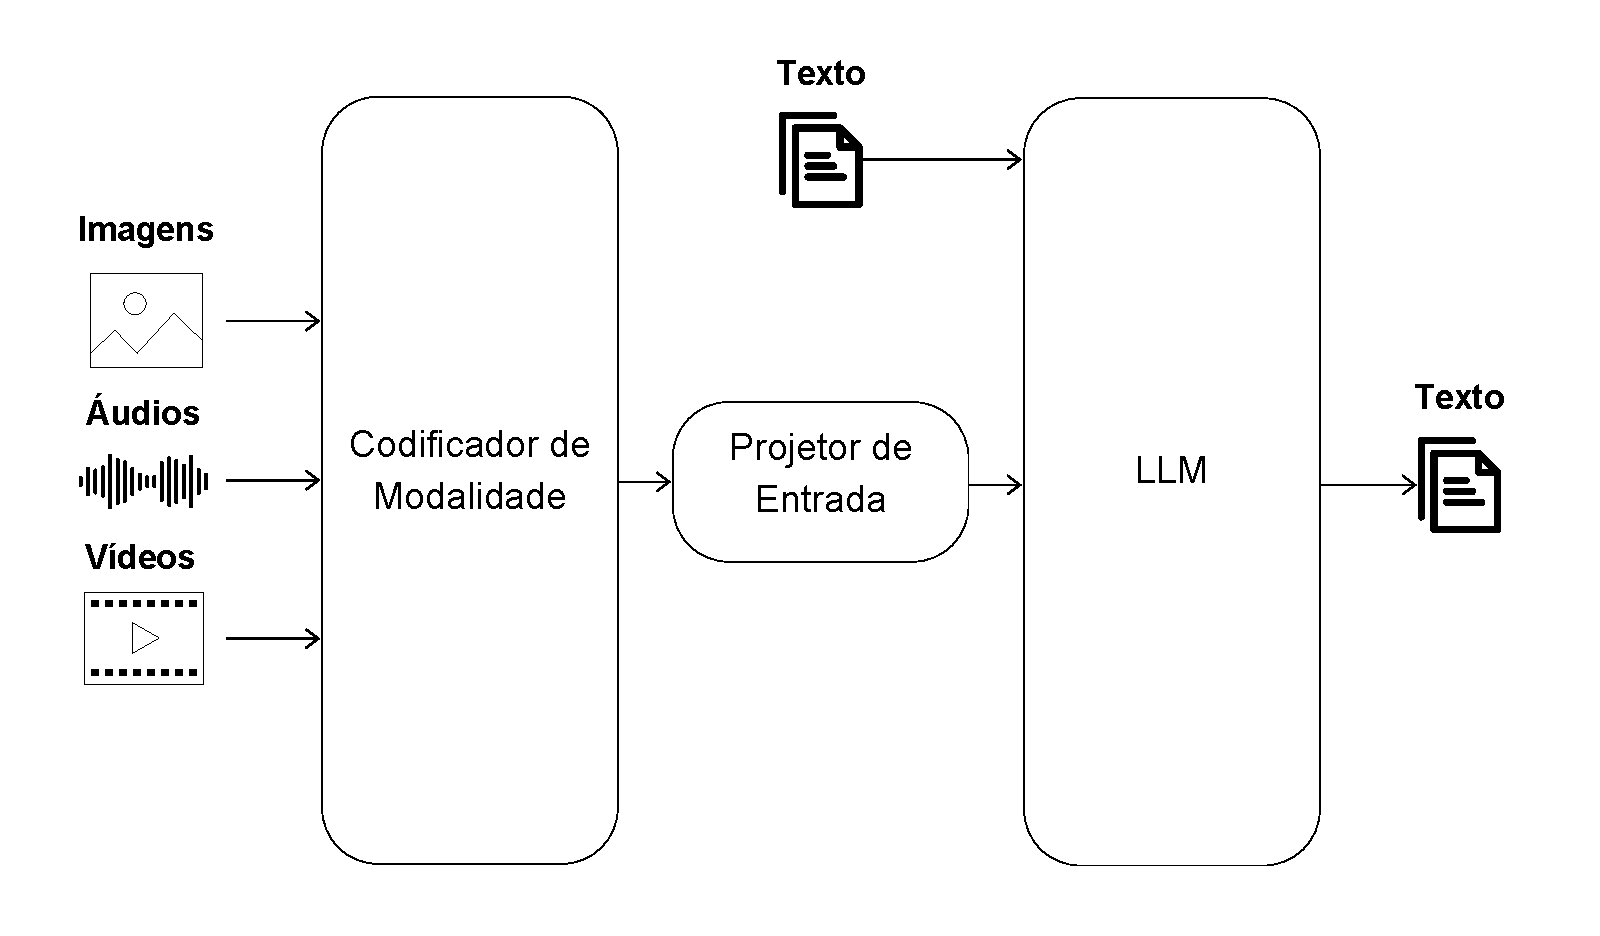
\includegraphics[width=0.7\columnwidth,keepaspectratio]{images/mllm_structure_encoder_only.pdf}
      \caption{\small Estrutura de um \ac{MLLM} que realiza apenas a interpretação multimodal.}
      \label{fig:mllm_structure_encoder_only}
\end{figure}

Neste trabalho, o foco será dado a modelos que interpretam imagens e retornam saídas textuais. Sendo assim, a parte de geração multimodal não será coberta.

\subsection{Large Language Models}

\acp{LLM} ou Grandes Modelos de Linguagem são modelos estatísticos pré-treinados baseados em transformadores capazes de processar e gerar textos em linguagem natural.

\subsubsection{Transformadores}

\subsubsubsection{Incorporação Vetorial}

Um \textit{embedding vector} ou uma incorporação vetorial é um vetor de valores reais em um espaço semântico n-dimensional que representa um dado, como, por exemplo, uma
palavra ou uma imagem. Esse tipo de representação permite que diferentes tipos de dados sejam representados em um espaço vetorial unificado. Na
\autoref{fig:word_embeddings} há um exemplo simplificado da estrutura destes vetores \cite{word_embedding, mllm_survey_2023}.

\begin{figure}[ht]
      \centering
      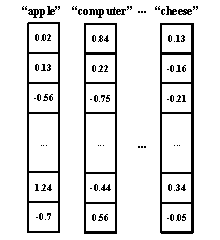
\includegraphics[width=0.4\columnwidth,keepaspectratio]{images/word_embeddings.pdf}
      \caption{\small Representação de palavras como vetores de valores reais. Fonte: \textcite{word_embedding}.}
      \label{fig:word_embeddings}
\end{figure}

Nesse espaço vetorial, direções podem ter um significado semântico. Um exemplo dado por \textcite{glove} demonstra isso com uma frase, traduzida do inglês: "Um rei é para
uma rainha o que um homem é para uma mulher", que pode ser representada como \textit{$V_{rei} - V_{rainha} \approx V_{homem} - V_{mulher}$}, evidenciando que a direção do
vetor \textit{$V_{rei} - V_{rainha}$} codifica informações sobre gênero. Além disso, a proximidade entre incorporações indica a similaridade semântica entre elas. Mais
exemplos dessa relação entre palavras podem ser vistos na \autoref{fig:word_embeddings_directions}.

\begin{figure}[ht]
      \centering
      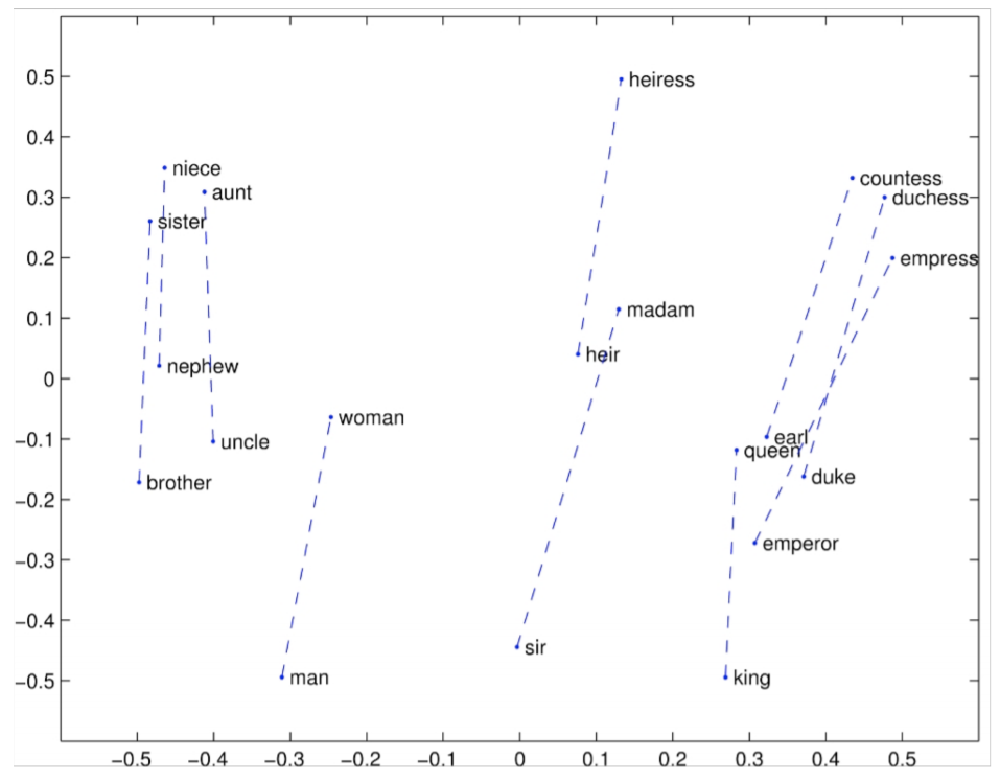
\includegraphics[width=0.7\columnwidth,keepaspectratio]{images/word_embeddings_directions.png}
      \caption{\small Visualização de incorporações com a direção que codifica informações de gênero evidenciada. Fonte: \textcite{word_embedding}.}
      \label{fig:word_embeddings_directions}
\end{figure}
\clearpage  % TODO: Apagar isso aqui se possível

\subsection{Codificador de Modalidade}

Codificadores de modalidade são os componentes responsáveis pela extração das características mais relevantes dos dados multimodais de entrada em incorporações vetoriais.
\cite{mllm_survey_2024}.

\subsubsection{Codificador Visual}

Existem diversos tipos de codificadores visuais. Os mais comuns usam \acp{ViT} ou Transformadores Visuais na suas arquiteturas, mas também há também codificadores
baseados em convolução \cite{mllm_survey_2023}. Neste trabalho o foco será direcionado a arquiteturas baseadas em \ac{ViT}.

\subsubsubsection{Transformadores Visuais}

\subsection{Projetor de Entrada}

\section{Fine-tuning}

\section{LLaMA}

\chapter{Trabalhos Correlatos} % TODO: Comentar mais sobre estudos que apresentam o impacto de diferentes técnicas de fine-tuning

Nesta seção serão apresentados os trabalhos similares a este para realizar comparações e apresentar melhor o estado da arte nessa linha de pesquisa.

\section{Classificação Automática de Lesões de Pele}

A utilização de \ac{IA} na detecção e classificação de lesões de pele tem se tornado cada vez mais relevante ao longo das últimas décadas. Historicamente, os maiores
avanços nessa área começaram com advento da aprendizagem profunda e das \acp{CNN} \cite{li2019artificial}. A maioria das técnicas tenta classificar o câncer de pele, mais
especificamente o melanoma, \ac{CBC} e \ac{CEC}. Porém, as técnicas desenvolvidas no contexto da classificação do câncer de pele também são úteis na classificação de
outras doenças \cite{okuboyejo2018review}.

O trabalho de \textcite{skin_cancer_ai} apresenta que os conjuntos de dados mais comuns na área são o \ac{HAM10000} e os fornecidos pela \ac{ISIC}. Além disso, \acp{CNN}
ainda dominam a área como a principal forma de implementar um sistema de classificação de lesões, atingindo entre 80\% e 99\% de acurácia. Cerca de 48,12\% dos conjuntos
de dados utilizam imagens de dermatoscopia, enquanto 33,33\% deles usam imagens macroscópicas, como as de aproximação e panorâmicas mencionadas na
\autoref{sec:skin_lesion_images}. Os outros 18,52\% se tratam de conjuntos com diversas modalidades de imagens, como imagens de ultrasonografia, multiespectrais e outras.

\section{Classificação com \textit{ViTs}}

Vários modelos de classificação de lesões baseados em \acp{ViT} foram propostos desde a introdução dessa arquitetura. A pesquisa de \textcite{khan2023identifying}
apresenta o cenário da utilização de \acp{ViT} nessa área. Muitas implementações seguem um modelo híbrido de \ac{ViT} e \ac{CNN}, combinando as capacidades das duas
arquiteturas.

Uma desvantagem das \acp{CNN} é a falta de entendimento de relações espaciais de longa distância em imagens de lesões de pele. Entretanto, \acp{ViT} conseguem resolver
esse problema, capturando as relações espaciais através do mecanismo de atenção. Mas, devido ao processo de divisão da imagem em seções de baixa resolução, \acp{ViT}
acabam tendo um desempenho pior, pois há uma perda de informações sobre detalhes mais finos. Nesse contexto, a utilização de modelos híbridos resolve esses problemas.
Uma dessas arquiteturas híbridas é a \textit{TransUNet}, combinando transformadores e \textit{U-Nets}, que conforme evidenciado por \textcite{gulzar2022skin}, consegue
atingir uma acurácia de 92,11\% na classificação de lesões de pele através do treinamento com o conjunto de dados \ac{ISIC}-2018.

\section{Classificação com \textit{MLLMs}}

\acp{MLLM} vêm sendo aplicados no contexto da dermatologia nos últimos anos. O \ac{GPT}-4V e o \ac{LLaVA} são dois modelos proeminentes na resolução de tarefas
visuais. Em um estudo de \textcite{cirone2024assessing}, é analisada a eficácia do uso desses modelos na identificação de melanomas em diferentes tons de pele.

Os testes foram feitos com os conjuntos de dados MClass-D, Dermnet NZ e imagens de livros de dermatologia, contendo imagens macroscópicas com resolução de
\begin{math}900 \times 1600\end{math} pixels. Para cada imagem, foram feitas 20 perguntas em relação às suas características, sendo que cada modelo foi testado com 3
imagens, resultando num total de 60 pares de pergunta e imagem por modelo. As imagens também tiveram suas cores modificadas para avaliar o impacto da coloração na
identificação de melanomas.

% TODO: Comentar sobre o modelo do Marques (http://sibgrapi.sid.inpe.br/col/sid.inpe.br/sibgrapi/2024/08.28.22.28/doc/Marques-125.pdf) e o SkinDiseaseChat

No fim, o \ac{GPT}-4V atingiu uma acurácia de 85\% e o \ac{LLaVA} atingiu apenas 45\%. O modelo \ac{LLaVA} não conseguiu identificar melanomas corretamente quando as
imagens tinham suas cores modificadas e também não conseguiu identificar detalhes como ulcerações ou sangramentos. Um detalhe importante é que ambos os modelos são
generalistas e não são treinados com um foco na classificação de lesões de pele.

O \textit{benchmark} OmniMedVQA de \textcite{hu2024omnimedvqa} traz dados sobre o desempenho de \acp{MLLM} em diferentes tarefas visuais da medicina. Em particular, os
testes apresentam as pontuações de diversos modelos na área de dermatologia, como pode ser visto na \autoref{tab:omnimedvqa_dermatology_results}.

\begin{table}[ht]
    \caption{\small Pontuação no \textit{benchmark} OmniMedVQA em dermatologia. A primeira seção de linhas contém modelos generalistas e a outra contém modelos
        especializados na área médica.}
    \centering
    \begin{tabular}{l|c}
        \hline
        Modelo                  & Pontuação em dermatologia \\ \hline
        InstructBLIP            & 61,86                     \\
        \ac{LLaMA}\_Adapter\_v2 & 51,43                     \\
        \ac{LLaVA}              & 49,67                     \\
        PGTrans                 & 44,66                     \\
        Otter                   & 42,66                     \\
        BLIP-2                  & 41,07                     \\
        Mini\ac{GPT}-4          & 40,09                     \\
        mPLUG-Owl               & 35,98                     \\ \hline
        \ac{LLaVA}-Med          & 44,90                     \\
        RadFM                   & 39,03                     \\
        Med-Flamingo            & 32,33                     \\
        MedVInT                 & 29,13                     \\ \hline
    \end{tabular}
    \label{tab:omnimedvqa_dermatology_results}
    \fonte{\textcite{hu2024omnimedvqa}}
\end{table}

Nas subseções abaixo, serão apresentados alguns modelos que focam em problemas relacionados à classificação de lesões de pele.

\subsection{SkinGPT-4}

Esse modelo foi proposto e desenvolvido por \textcite{zhou2023skingpt} e se baseia no Mini\ac{GPT}-4, um \ac{MLLM} composto por um \ac{ViT} com um \textit{Q-Former}
pré-treinado e o \ac{LLM} Vicuna, que por sua vez é baseado no \ac{LLaMA}. A arquitetura pode ser vista na \autoref{fig:skingpt4}.

\begin{figure}[ht]
    \centering
    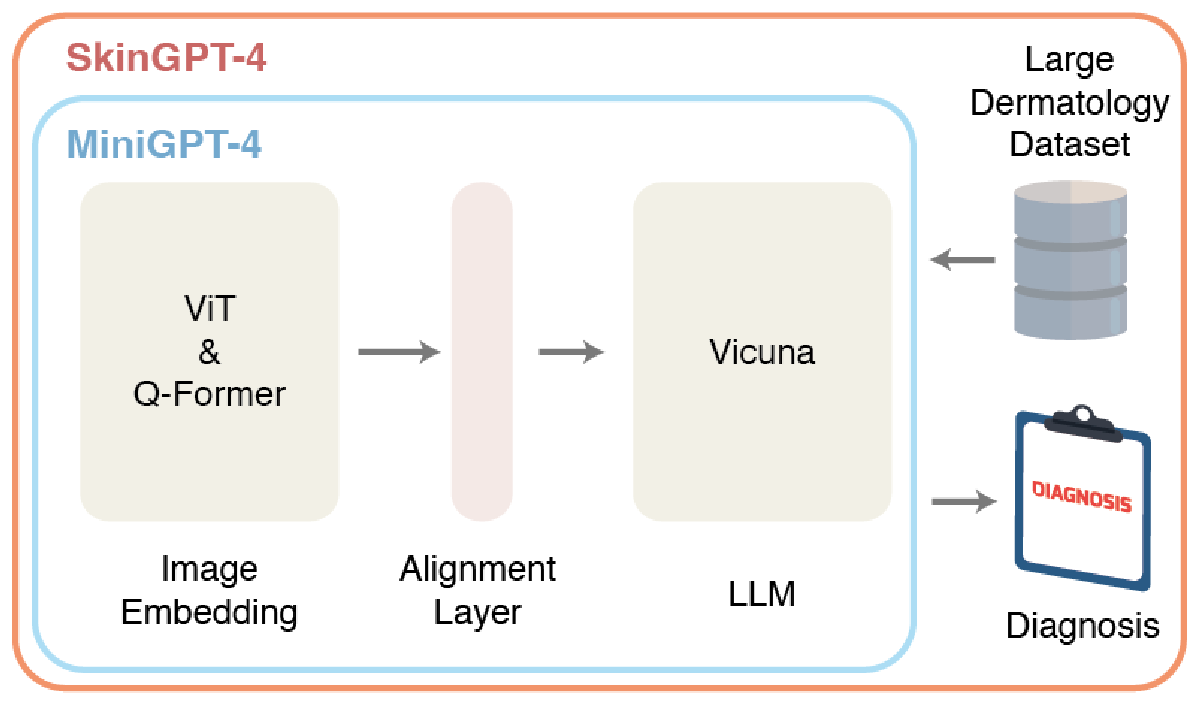
\includegraphics[width=0.55\columnwidth,keepaspectratio]{images/skingpt4.png}
    \caption{\small Arquitetura do Skin\ac{GPT}-4. Fonte: \textcite{zhou2023skingpt}.}
    \label{fig:skingpt4}
\end{figure}

Nesse estudo, o Mini\ac{GPT}-4 passou por um processo de \textit{fine-tuning} de duas etapas que familiarizou o modelo com imagens de lesões de pele e depois ajustou suas
saídas para um formato mais próximo de um diagnóstico médico. As imagens vieram de um conjunto de dados particular, do SKINCON e do Dermnet, sendo que 3886 imagens foram
usadas na primeira etapa de treinamento e 49043 na segunda.

A verificação do desempenho do modelo foi feito com base em 150 diagnósticos de casos reais realizados pelo Skin\ac{GPT}-4. Esses diagnósticos foram avaliados por
dermatologistas certificados, sendo que 78,76\% dos diagnósticos foram classificados como corretos.

\subsection{LLaVA-Med}

O \ac{LLaVA}-Med é um modelo com foco na área médica geral desenvolvido por \textcite{li2024llava}. Esse modelo é baseado no \ac{LLaVA}, sendo composto pelo \ac{LLM}
Vicuna e o codificador visual \ac{CLIP} \ac{ViT}-L/14 \cite{liu2024visual}.

Foram criados dois conjuntos de dados com base em pares de imagens e textos de diversas áreas da medicina, um conjunto para alinhamento de conceitos e outro para
\textit{instruction-following}. A primeira etapa do treinamento envolveu o \textit{fine-tuning} do projetor de entrada por 7 horas em 8 NVIDIA A100 de 40 GB, alinhando
o modelo com o contexto médico. Já a segunda etapa levou 8 horas com as mesmas GPUs, realizando o \textit{fine-tuning} sobre o projetor de entrada e o \ac{LLM}, adaptando
o modelo para responder perguntas sobre imagens de casos médicos.

Esse modelo apresentou um desempenho melhor em relação ao \ac{LLaVA} original, atingindo mais de 90 pontos no \textit{benchmark} PathVQA, por exemplo.

\subsection{MpoxVLM}

O modelo MpoxVLM de \textcite{cao2024mpoxvlm} é um \ac{MLLM} direcionado ao diagnóstico de lesões de pele causadas pela doença \textit{Monkeypox}. O modelo possui dois
codificadores visuais, um deles é o \ac{CLIP} \ac{ViT}-L/14 e o outro é o \ac{ViT}-L/14-336 pré-treinado para a classificação de lesões de pele. Um \ac{MLP} de duas camadas
é usado como projetor de entrada para o codificador \ac{CLIP}, sendo que a saída do codificador \ac{ViT}, a classe da lesão de pele, é enviada para outro projetor de
entrada. O \ac{LLaMA}-2 é usado como \ac{LLM}, especificamente a variante com 7 bilhões de parâmetros. A \autoref{fig:mpoxvlm} apresenta a arquitetura deste \ac{MLLM}.

\begin{figure}[ht]
    \centering
    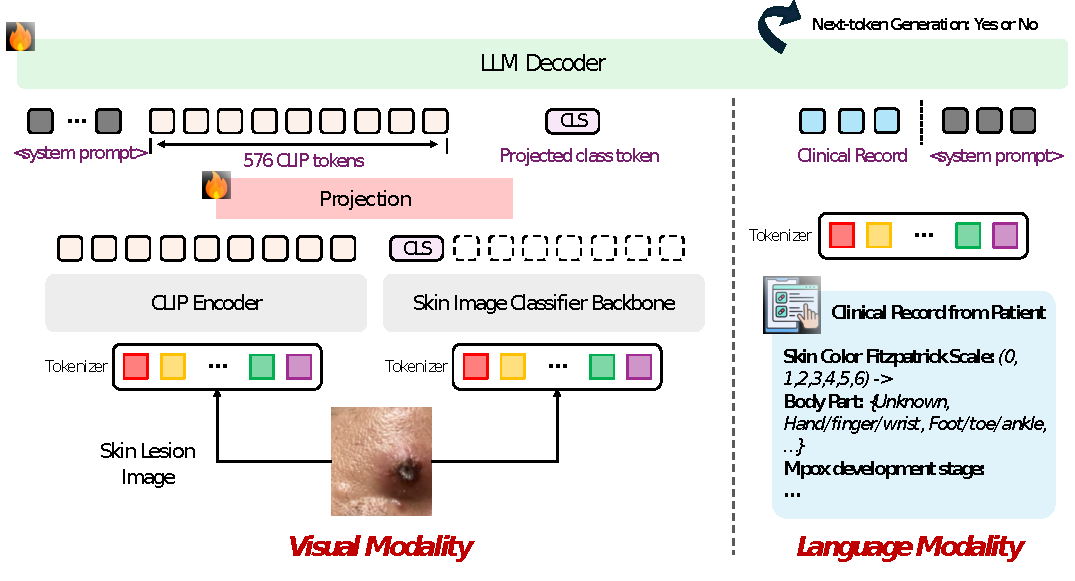
\includegraphics[width=0.85\columnwidth,keepaspectratio]{images/mpoxvlm.pdf}
    \caption{\small Arquitetura do MpoxVLM. Fonte: \textcite{cao2024mpoxvlm}.}
    \label{fig:mpoxvlm}
\end{figure}

Inicialmente, o \ac{ViT}-L/14-336 foi pré-treinado com o conjunto de dados de lesões de pele causadas por \textit{Monkeypox}. Depois o modelo foi construído e os
projetores de entrada foram treinados. Por fim, foi feito um \textit{fine-tuning} com \ac{LoRA} do \ac{LLaMA}-2 para tarefas de pergunta e resposta. Foram utilizadas
duas NVIDIA RTX 4090 para os treinamentos nesse estudo.

Os resultados apresentados demonstram que o MpoxVLM atinge uma acurácia de 90,38\% no diagnóstico de \textit{Monkeypox}, ultrapassando vários outros \acp{MLLM}.

\subsection{Comparação entre \textit{MLLMs}} % TODO: Comentar que no paper do LLaMA-3.2 viram que CLIP não é tão bom assim

Em geral, os modelos utilizam como base \acp{LLM} da família \ac{LLaMA} e codificadores visuais baseados em \acp{ViT}, sendo que o MpoxVLM apresentou a arquitetura
mais complexa. O \textit{fine-tuning} completo também é frequentemente utilizado, porém, o MpoxVLM atingiu bons resultados com o \ac{LoRA}. Dos três modelos apresentados,
somente o Skin\ac{GPT}-4 e o MpoxVLM são especializados em lesões de pele, sendo que o artigo do Skin\ac{GPT}-4 é o que tem o objetivo mais similar ao deste trabalho. Os
conjuntos de dados utilizados são diversos e possuem imagens de diferentes categorias, como macroscópicas e dermatoscópicas.

Devido a recência do \ac{LLaMA}-3.2, há poucos casos em que este modelo foi utilizado. Um diferencial considerável deste trabalho é a utilização deste \ac{MLLM}. Outro
diferencial é a análise da eficácia do \ac{QLoRA} em relação ao \ac{LoRA} no contexto de classificação de lesões de pele. A \autoref{tab:mllm_comparison} mostra uma
comparação entre os \acp{MLLM} apresentados.

\begin{table}[ht]
    \caption{\small Comparação entre diferentes \acp{MLLM} focados na área médica e na classificação de lesões de pele.}
    \centering
    \begin{tabular}{l|cc}
        \hline
        Modelo                & MLLM base ou arquitetura                  & Treinamento            \\ \hline
        Skin\ac{GPT}-4        & Mini\ac{GPT}-4                            & Fine-tuning completo   \\
        \ac{LLaVA}-Med        & \ac{LLaVA}                                & Fine-tuning completo   \\
        MpoxVLM               & \ac{CLIP}, \ac{ViT}-L/14-336 e LLaMA-2-7B & \ac{LoRA}              \\
        Modelo deste trabalho & \ac{LLaMA}-3.2-11B e \ac{LLaMA}-3.2-90B   & \ac{QLoRA} e \ac{LoRA} \\ \hline
    \end{tabular}
    \label{tab:mllm_comparison}
    \fonte{Autoria própria.}
\end{table}
\chapter{Desenvolvimento Parcial} % TODO: Melhorar isso no futuro e resumir a primeira parte

Esta seção apresenta a etapa inicial de \textit{fine-tuning} do \ac{LLaMA}-3.2, sendo que ela tem um caráter exploratório e visa o desenvolvimento do código base para
os próximos experimentos e também analisar a capacidade de classificação do modelo treinado de diferentes formas.

\section{Tecnologias Utilizadas}

O processamento de dados e \textit{fine-tuning} foram feitos com \textit{scripts} em Python e \textit{Jupyter notebooks}. As dependências do projeto foram gerenciadas
com o gerenciador Poetry e o \textit{framework} de \textit{fine-tuning} utilizado foi o Unsloth. Os treinamentos foram realizados com uma placa NVIDIA H100 de 80 GB que
faz parte de uma plataforma NVIDIA DGX H100.

\section{Conjunto de Dados}

Para os experimentos inciais, utilizou-se o conjunto de dados \ac{HAM10000} de \textcite{tschandl2018ham10000}, que possui 13354 imagens com informações como a doença
causadora da lesão de pele, a idade do paciente, sexo e localização da lesão. As imagens nesse conjunto de dados são de dermatoscopia.

O conjunto de dados é separado nas seções de treinamento, teste e validação, que possuem 9577, 1285 e 2492 imagens, respectivamente. A \autoref{tab:ham10000_proportion}
apresenta as proporções entre as categorias de lesões de pele. Os dados foram obtidos a partir da plataforma Hugging Face com uma versão do \ac{HAM10000} fornecida por
\textcite{skin_cancer_dataset}.

\begin{table}[ht]
    \caption{\small Proporção entre as diferentes categorias de lesões de pele no \ac{HAM10000}.}
    \centering
    \begin{tabular}{l|c}
        \hline
        Lesão de pele                        & Proporção (\%) \\ \hline
        Nevo melanocítico                    & 66,88          \\
        Melanoma                             & 11,23          \\
        Lesões similares à queratose benigna & 10,94          \\
        \ac{CBC}                             & 5,08           \\
        Queratose actínica                   & 3,29           \\
        Lesões vasculares                    & 1,42           \\
        Dermatofibroma                       & 1,15           \\ \hline
    \end{tabular}
    \label{tab:ham10000_proportion}
    \fonte{\textcite{tschandl2018ham10000}}
\end{table}

\section{Experimentos com \textit{Fine-tuning}}

Os experimentos utilizaram a variante \ac{LLaMA}-3.2-11B-Vision-Instruct, que possui 11 bilhões de parâmetros. Os métodos de \textit{fine-tuning} utilizados foram o
\ac{LoRA} e o \ac{QLoRA}.

\subsection{Dados de treinamento}

O modelo utilizado não suporta ainda a utilização de textos em português para tarefas multimodais, sendo assim, os diálogos estão em inglês. Foi aplicada uma amostragem
estratificada por categoria de lesão de pele sobre os dados de treinamento para que os diálogos tivessem uma representação proporcional de cada lesão. Eles possuem o
seguinte formato:

\begin{dialogue}
    \speak{Usuário} \textit{Classify the skin lesion in the image. \textbf{<imagem>}} \\
    \speak{Modelo} \textit{The skin lesion in the image is \textbf{<lesão de pele>}.}
\end{dialogue}

\subsection{\textit{Fine-tuning} com 450, 900 e 1800 amostras}

% TODO: Ver se é necessário citar os criadores do Adam e AdamW.

A primeira etapa nos experimentos realizar o \textit{fine-tuning} com \ac{QLoRA} com 450 amostras de treinamento e 50 de validação. Os hiperparâmetros\footnote{parâmetros
    de treinamento} utilizados no treinamento estão na \autoref{tab:qlora_500_config}, alguns deles foram omitidos por serem menos relevantes nessa etapa. O \ac{rsLoRA} de
\textcite{kalajdzievski2023rank} foi utilizado para melhorar o desempenho, utilizando um fator de escala \begin{math}\frac{\alpha_{LoRA}}{\sqrt{r}}\end{math} em vez do
\begin{math}\frac{\alpha_{LoRA}}{r}\end{math} do \ac{LoRA} original. Por fim, também foi utilizado o otimizador \ac{Adam} na sua versão paginada de 32 bits. A
\autoref{tab:qlora_500_training} apresenta dados sobre o treinamento e a \autoref{fig:loss_qlora_500} apresenta o \textit{loss} de treinamento e validação ao longo dos
passos.

\begin{table}[ht]
    \caption{\small Hiperparâmetros para o \ac{QLoRA} com 450, 900 e 1800 amostras. A primeira seção se refere às configurações específicas de \ac{PEFT}, enquanto a
        segunda se refere ao treinamento em geral.}
    \centering
    \begin{tabular}{l|c}
        \hline
        Hiperparâmetro                             & Valor                                  \\ \hline
        Camadas e módulos treinados                & Visão, linguagem, atenção e \ac{MLP}   \\
        Rank                                       & 32                                     \\
        Alfa (\begin{math}\alpha_{LoRA}\end{math}) & 32                                     \\
        Dropout                                    & 0,1                                    \\
        \ac{rsLoRA}                                & Sim                                    \\ \hline
        Taxa de aprendizado                        & \begin{math}2 \times 10^{-4}\end{math} \\
        Razão de aquecimento                       & 0,03                                   \\
        Tipo de escalonador da taxa de aprendizado & Cosseno com reinícios                  \\
        Decaimento de peso                         & 0,01                                   \\
        Épocas                                     & 5                                      \\
        Passos a cada validação                    & 50                                     \\
        Otimizador                                 & \ac{Adam} paginado de 32 bits          \\
        Tipo numérico                              & \ac{BF16}                              \\ \hline
    \end{tabular}
    \label{tab:qlora_500_config}
    \fonte{Autoria própria}
\end{table}

\begin{table}[ht]
    \caption{\small Dados sobre o treinamento com \ac{QLoRA} com 450 amostras.}
    \centering
    \begin{tabular}{l|c}
        \hline
                                    & Valor     \\ \hline
        Parâmetros treináveis       & 134348800 \\
        Tempo de treinamento (min)  & 16,17     \\
        Passos                      & 110       \\
        Memória máxima alocada (GB) & 18.69     \\ \hline
    \end{tabular}
    \label{tab:qlora_500_training}
    \fonte{Autoria própria}
\end{table}

\begin{figure}[ht]
    \centering
    \caption{\small \textit{Loss} de treinamento e validação para o \ac{QLoRA} com 450 amostras.}
    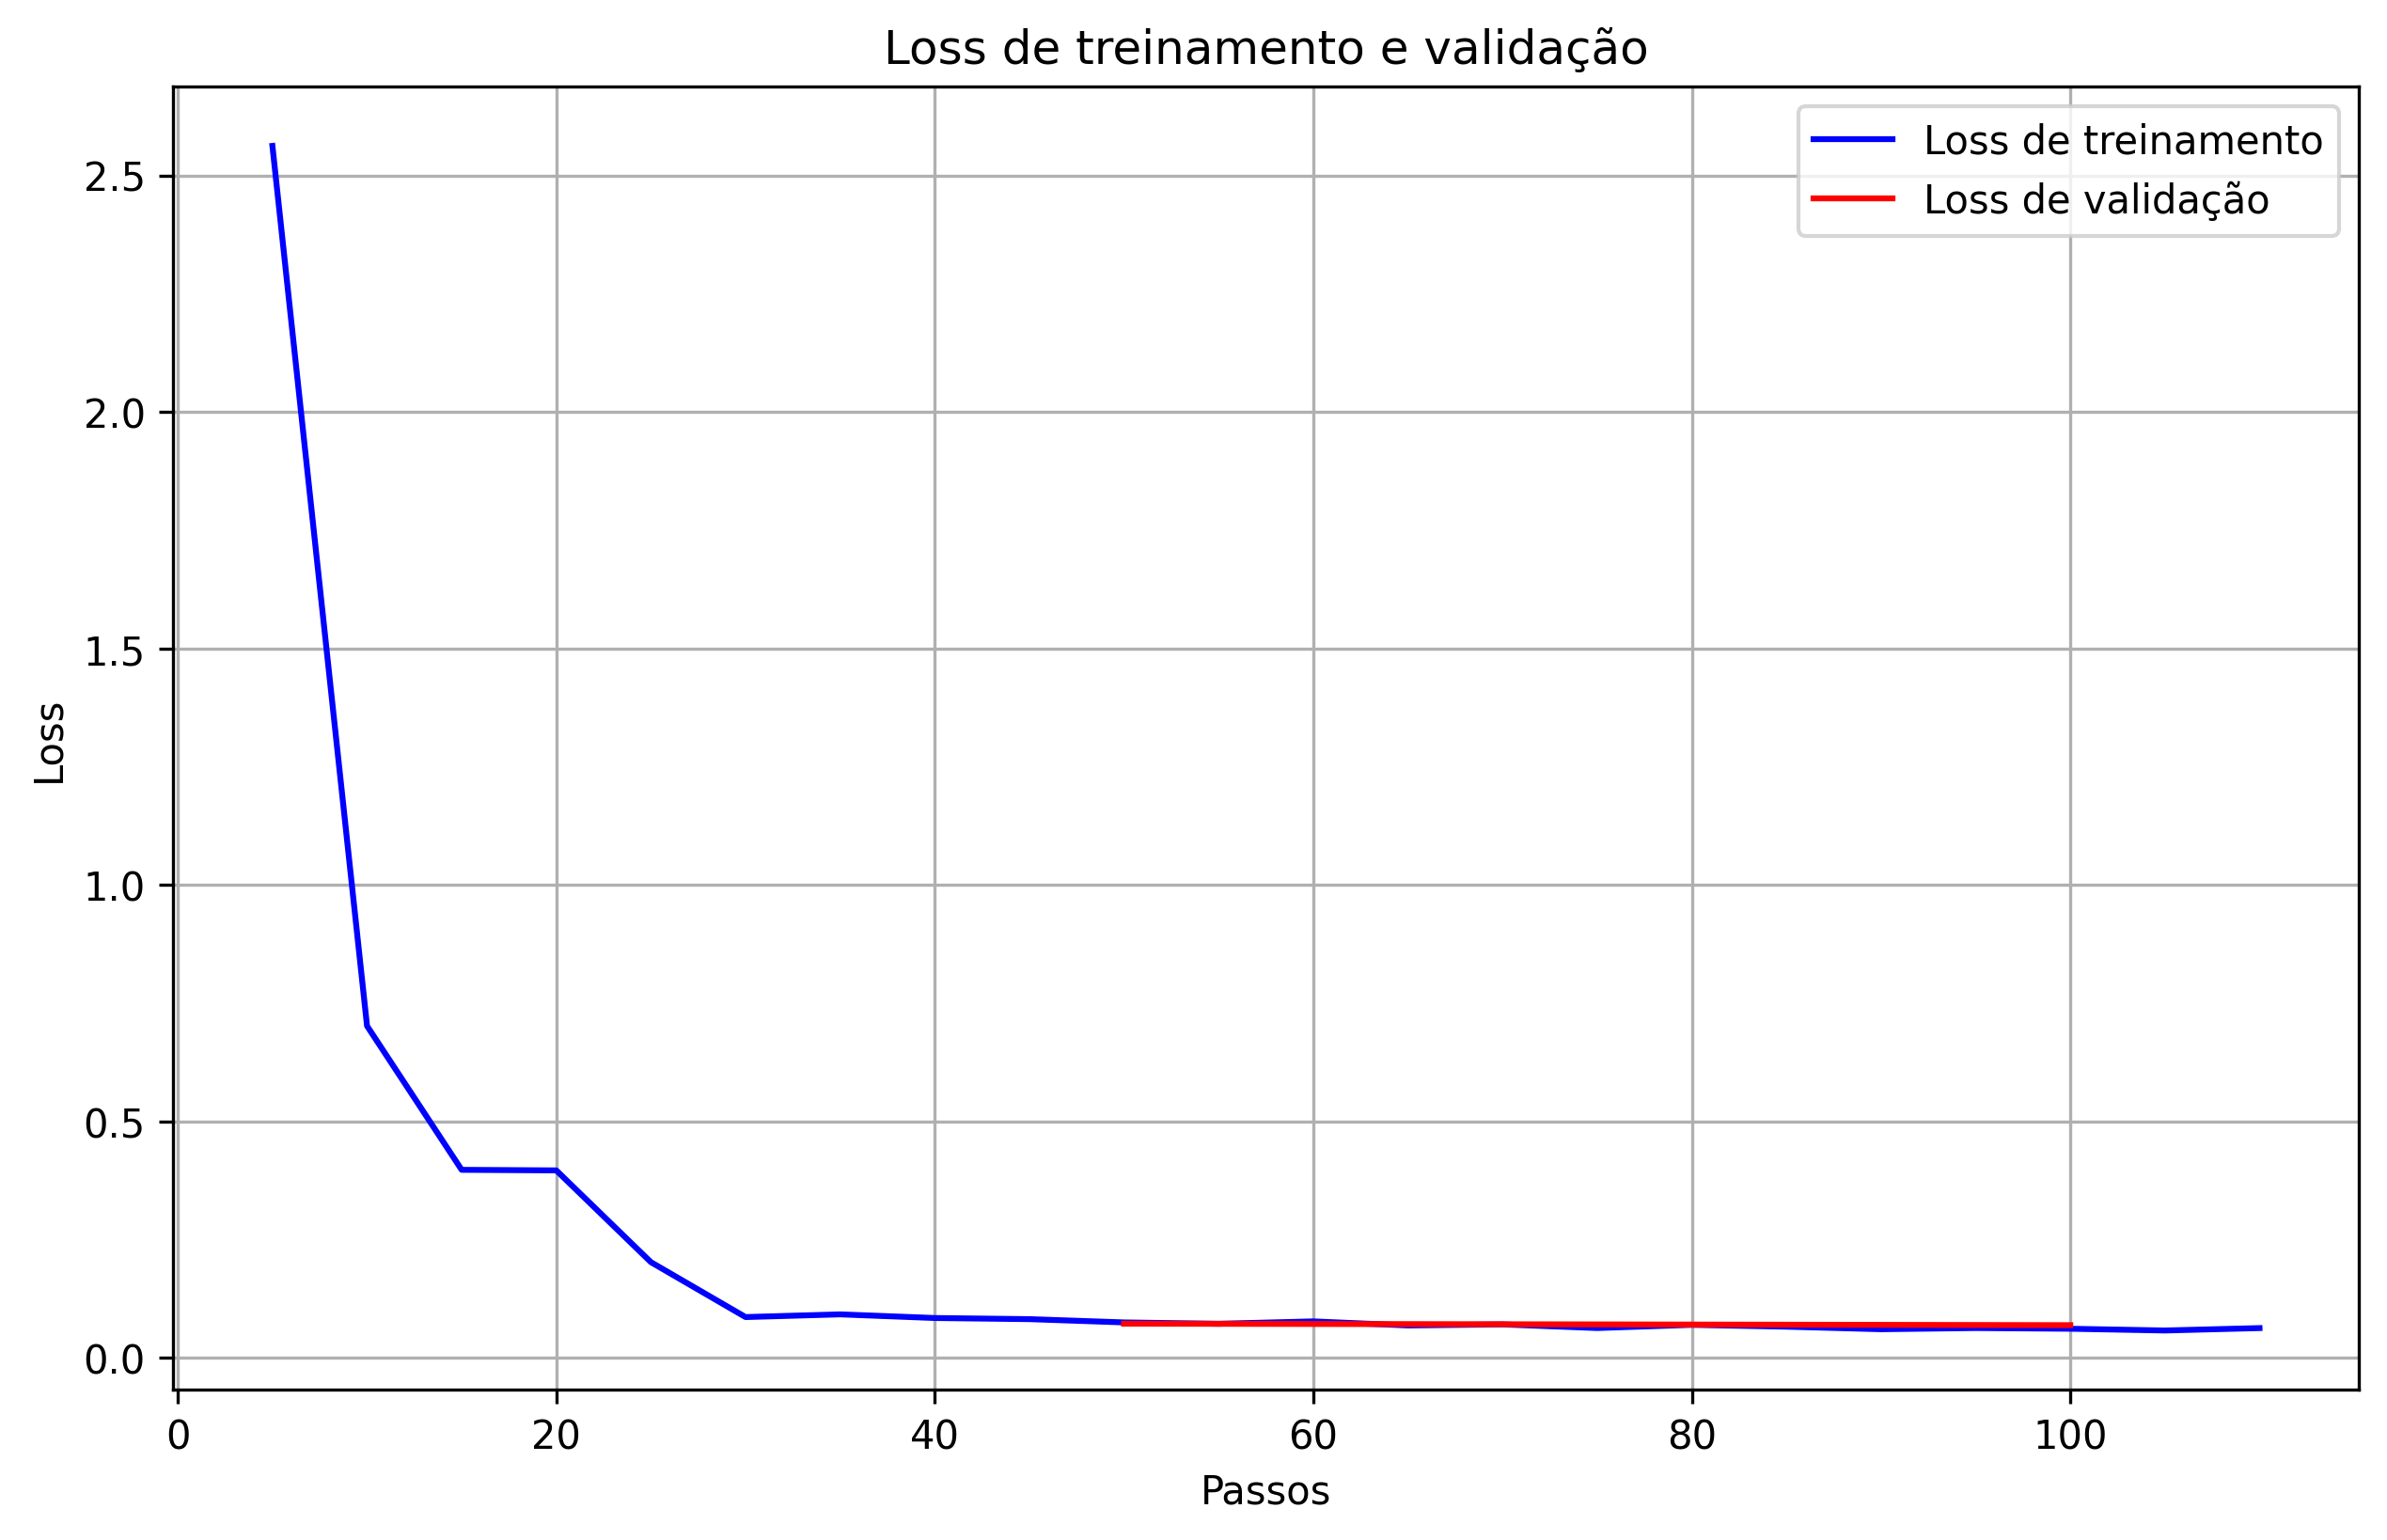
\includegraphics[width=0.8\columnwidth,keepaspectratio]{images/loss_qlora_500.png}
    \label{fig:loss_qlora_500}
    \fonte{Autoria própria.}
\end{figure}

Em seguida, foi realizado o \textit{fine-tuning} com \ac{LoRA}, ou seja, sem quantização, com 450 amostras. Os hiperparâmetros utilizados são similares, porém, o
\textit{rank} foi reduzido para 16, assim como o \begin{math}\alpha_{LoRA}\end{math}. O \ac{rsLoRA} não foi utilizado e a taxa de aprendizado foi reduzida a
\begin{math}1 \times 10^{-4}\end{math}. Por fim o otimizador \ac{AdamW} foi utilizado. A \autoref{tab:lora_500_training} apresenta os dados de treinamento e a
\autoref{fig:loss_lora_500} apresenta o \textit{loss}. O treinamento foi aplicado somente sobre 64174400 parâmetros, uma quantidade menor do que a usada no
\ac{QLoRA} por conta do \textit{rank} reduzido.

\begin{table}[ht]
    \caption{\small Dados sobre o treinamento com \ac{LoRA} com 450 amostras.}
    \centering
    \begin{tabular}{l|c}
        \hline
                                    & Valor    \\ \hline
        Parâmetros treináveis       & 64174400 \\
        Tempo de treinamento (min)  & 26,42    \\
        Passos                      & 140      \\
        Memória máxima alocada (GB) & 40,35    \\ \hline
    \end{tabular}
    \label{tab:lora_500_training}
    \fonte{Autoria própria}
\end{table}

\clearpage

\begin{figure}[ht]
    \centering
    \caption{\small \textit{Loss} de treinamento e validação para o \ac{LoRA} com 450 amostras.}
    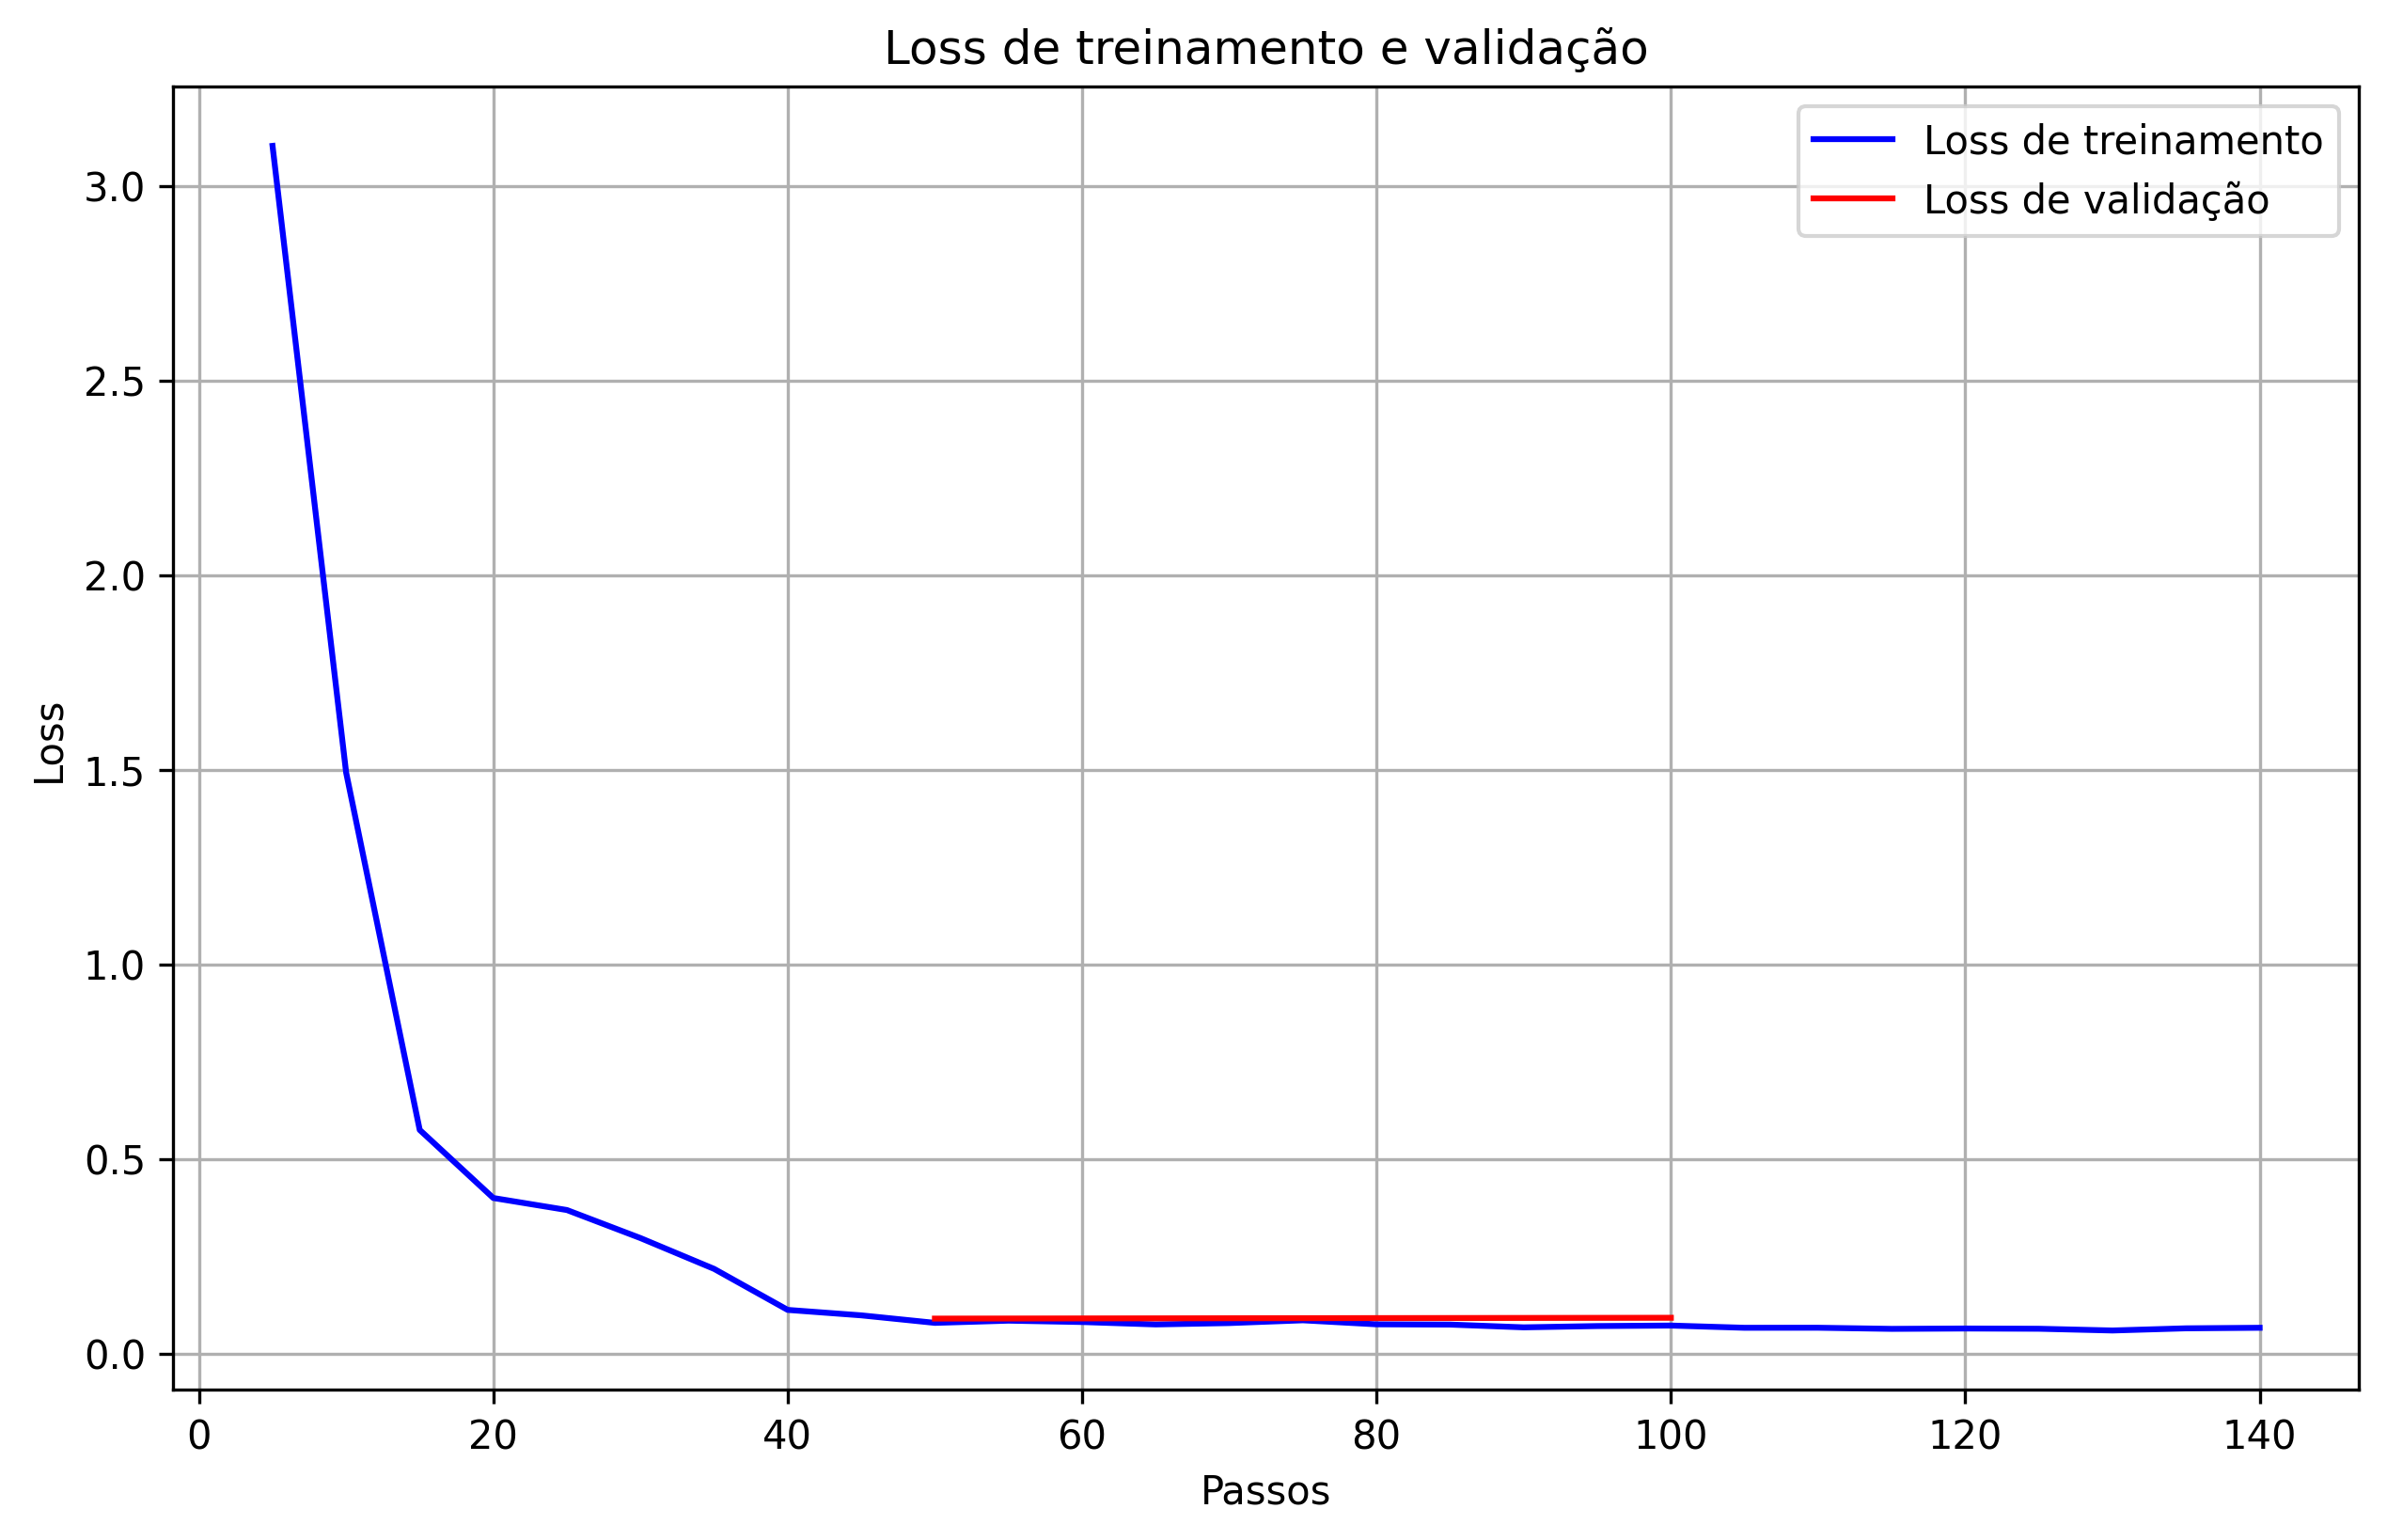
\includegraphics[width=0.725\columnwidth,keepaspectratio]{images/loss_lora_500.png}
    \label{fig:loss_lora_500}
    \fonte{Autoria própria.}
\end{figure}

O \textit{fine-tuning} com 900 amostras foi feito sem a alteração nos hiperparâmetros do \ac{QLoRA} e \ac{LoRA}. As informações sobre o treinamento podem ser conferidas
na \autoref{tab:qlora_1000_training} e \autoref{tab:lora_1000_training}, enquanto o \textit{loss} pode ser conferido na \autoref{fig:loss_qlora_1000} e
\autoref{fig:loss_lora_1000}.

\begin{table}[ht]
    \caption{\small Dados sobre o treinamento com \ac{QLoRA} com 900 amostras.}
    \centering
    \begin{tabular}{l|c}
        \hline
                                    & Valor     \\ \hline
        Parâmetros treináveis       & 134348800 \\
        Tempo de treinamento (min)  & 32,08     \\
        Passos                      & 225       \\
        Memória máxima alocada (GB) & 18,695    \\ \hline
    \end{tabular}
    \label{tab:qlora_1000_training}
    \fonte{Autoria própria}
\end{table}

\begin{table}[ht]
    \caption{\small Dados sobre o treinamento com \ac{LoRA} com 900 amostras.}
    \centering
    \begin{tabular}{l|c}
        \hline
                                    & Valor    \\ \hline
        Parâmetros treináveis       & 67174400 \\
        Tempo de treinamento (min)  & 41,76    \\
        Passos                      & 280      \\
        Memória máxima alocada (GB) & 31,965   \\ \hline
    \end{tabular}
    \label{tab:lora_1000_training}
    \fonte{Autoria própria}
\end{table}

\clearpage

\begin{figure}[ht]
    \centering
    \caption{\small \textit{Loss} de treinamento e validação para o \ac{QLoRA} com 900 amostras.}
    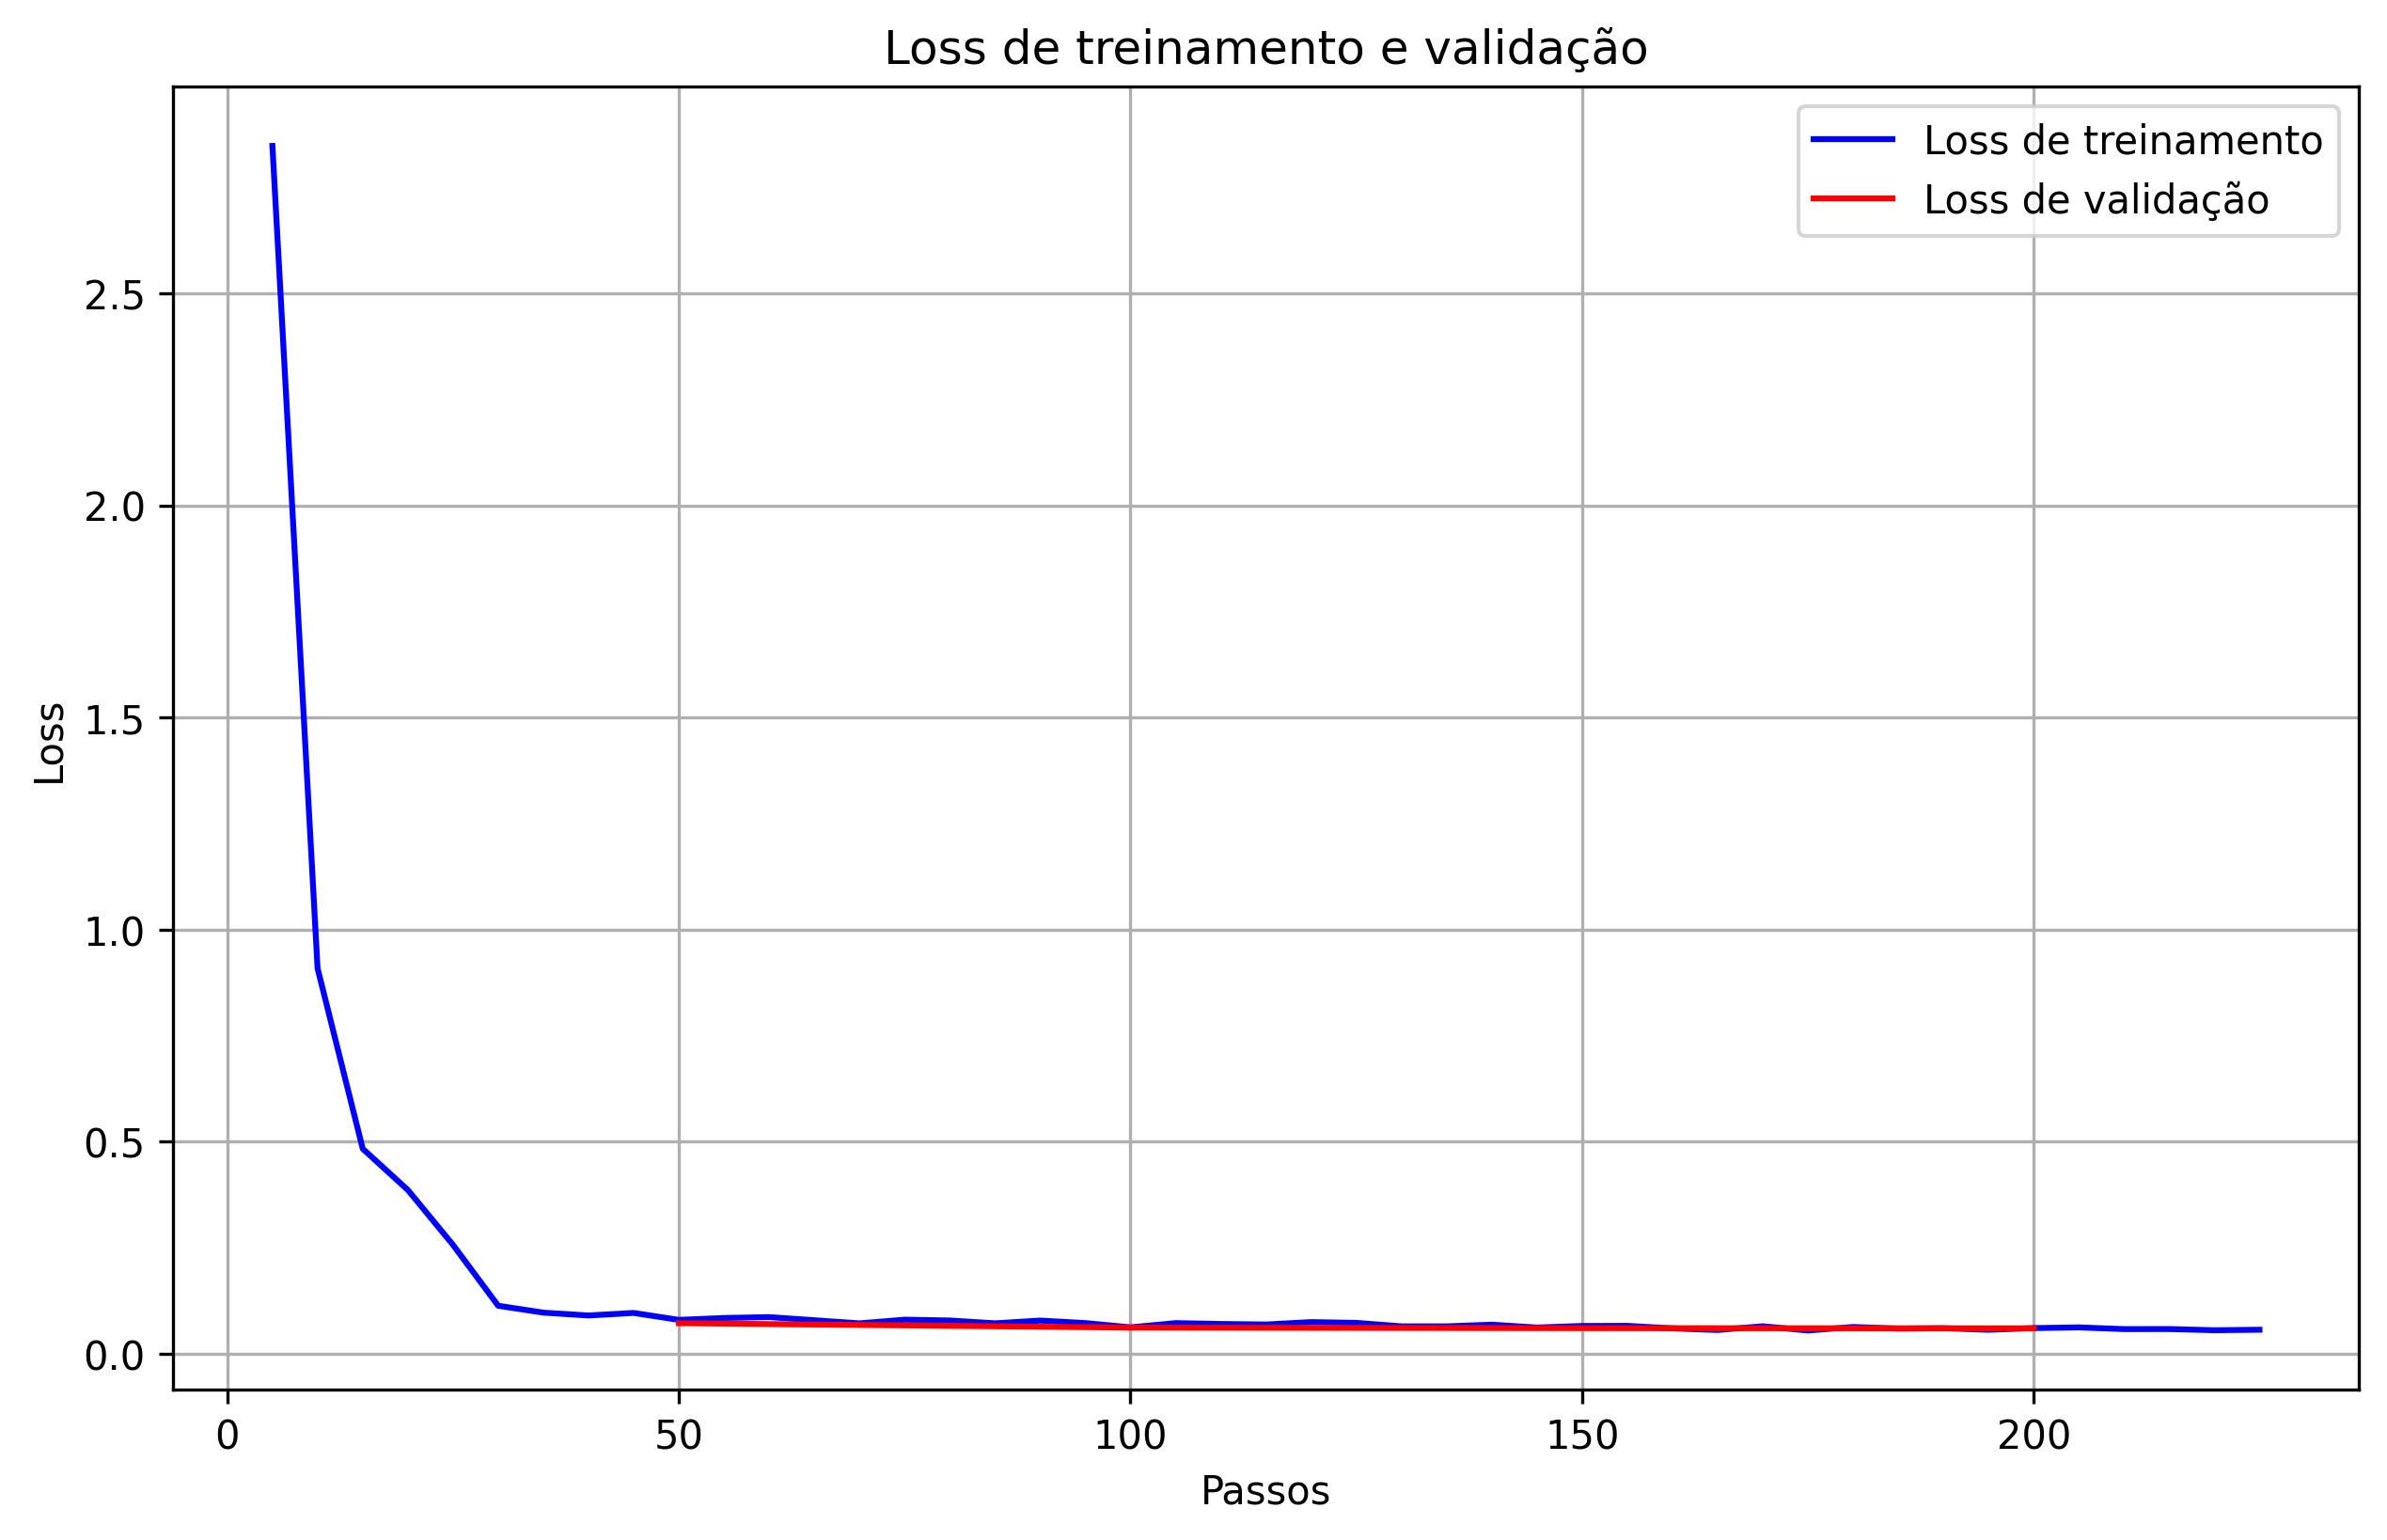
\includegraphics[width=0.725\columnwidth,keepaspectratio]{images/loss_qlora_1000.png}
    \label{fig:loss_qlora_1000}
    \fonte{Autoria própria.}
\end{figure}

\begin{figure}[ht]
    \centering
    \caption{\small \textit{Loss} de treinamento e validação para o \ac{LoRA} com 900 amostras.}
    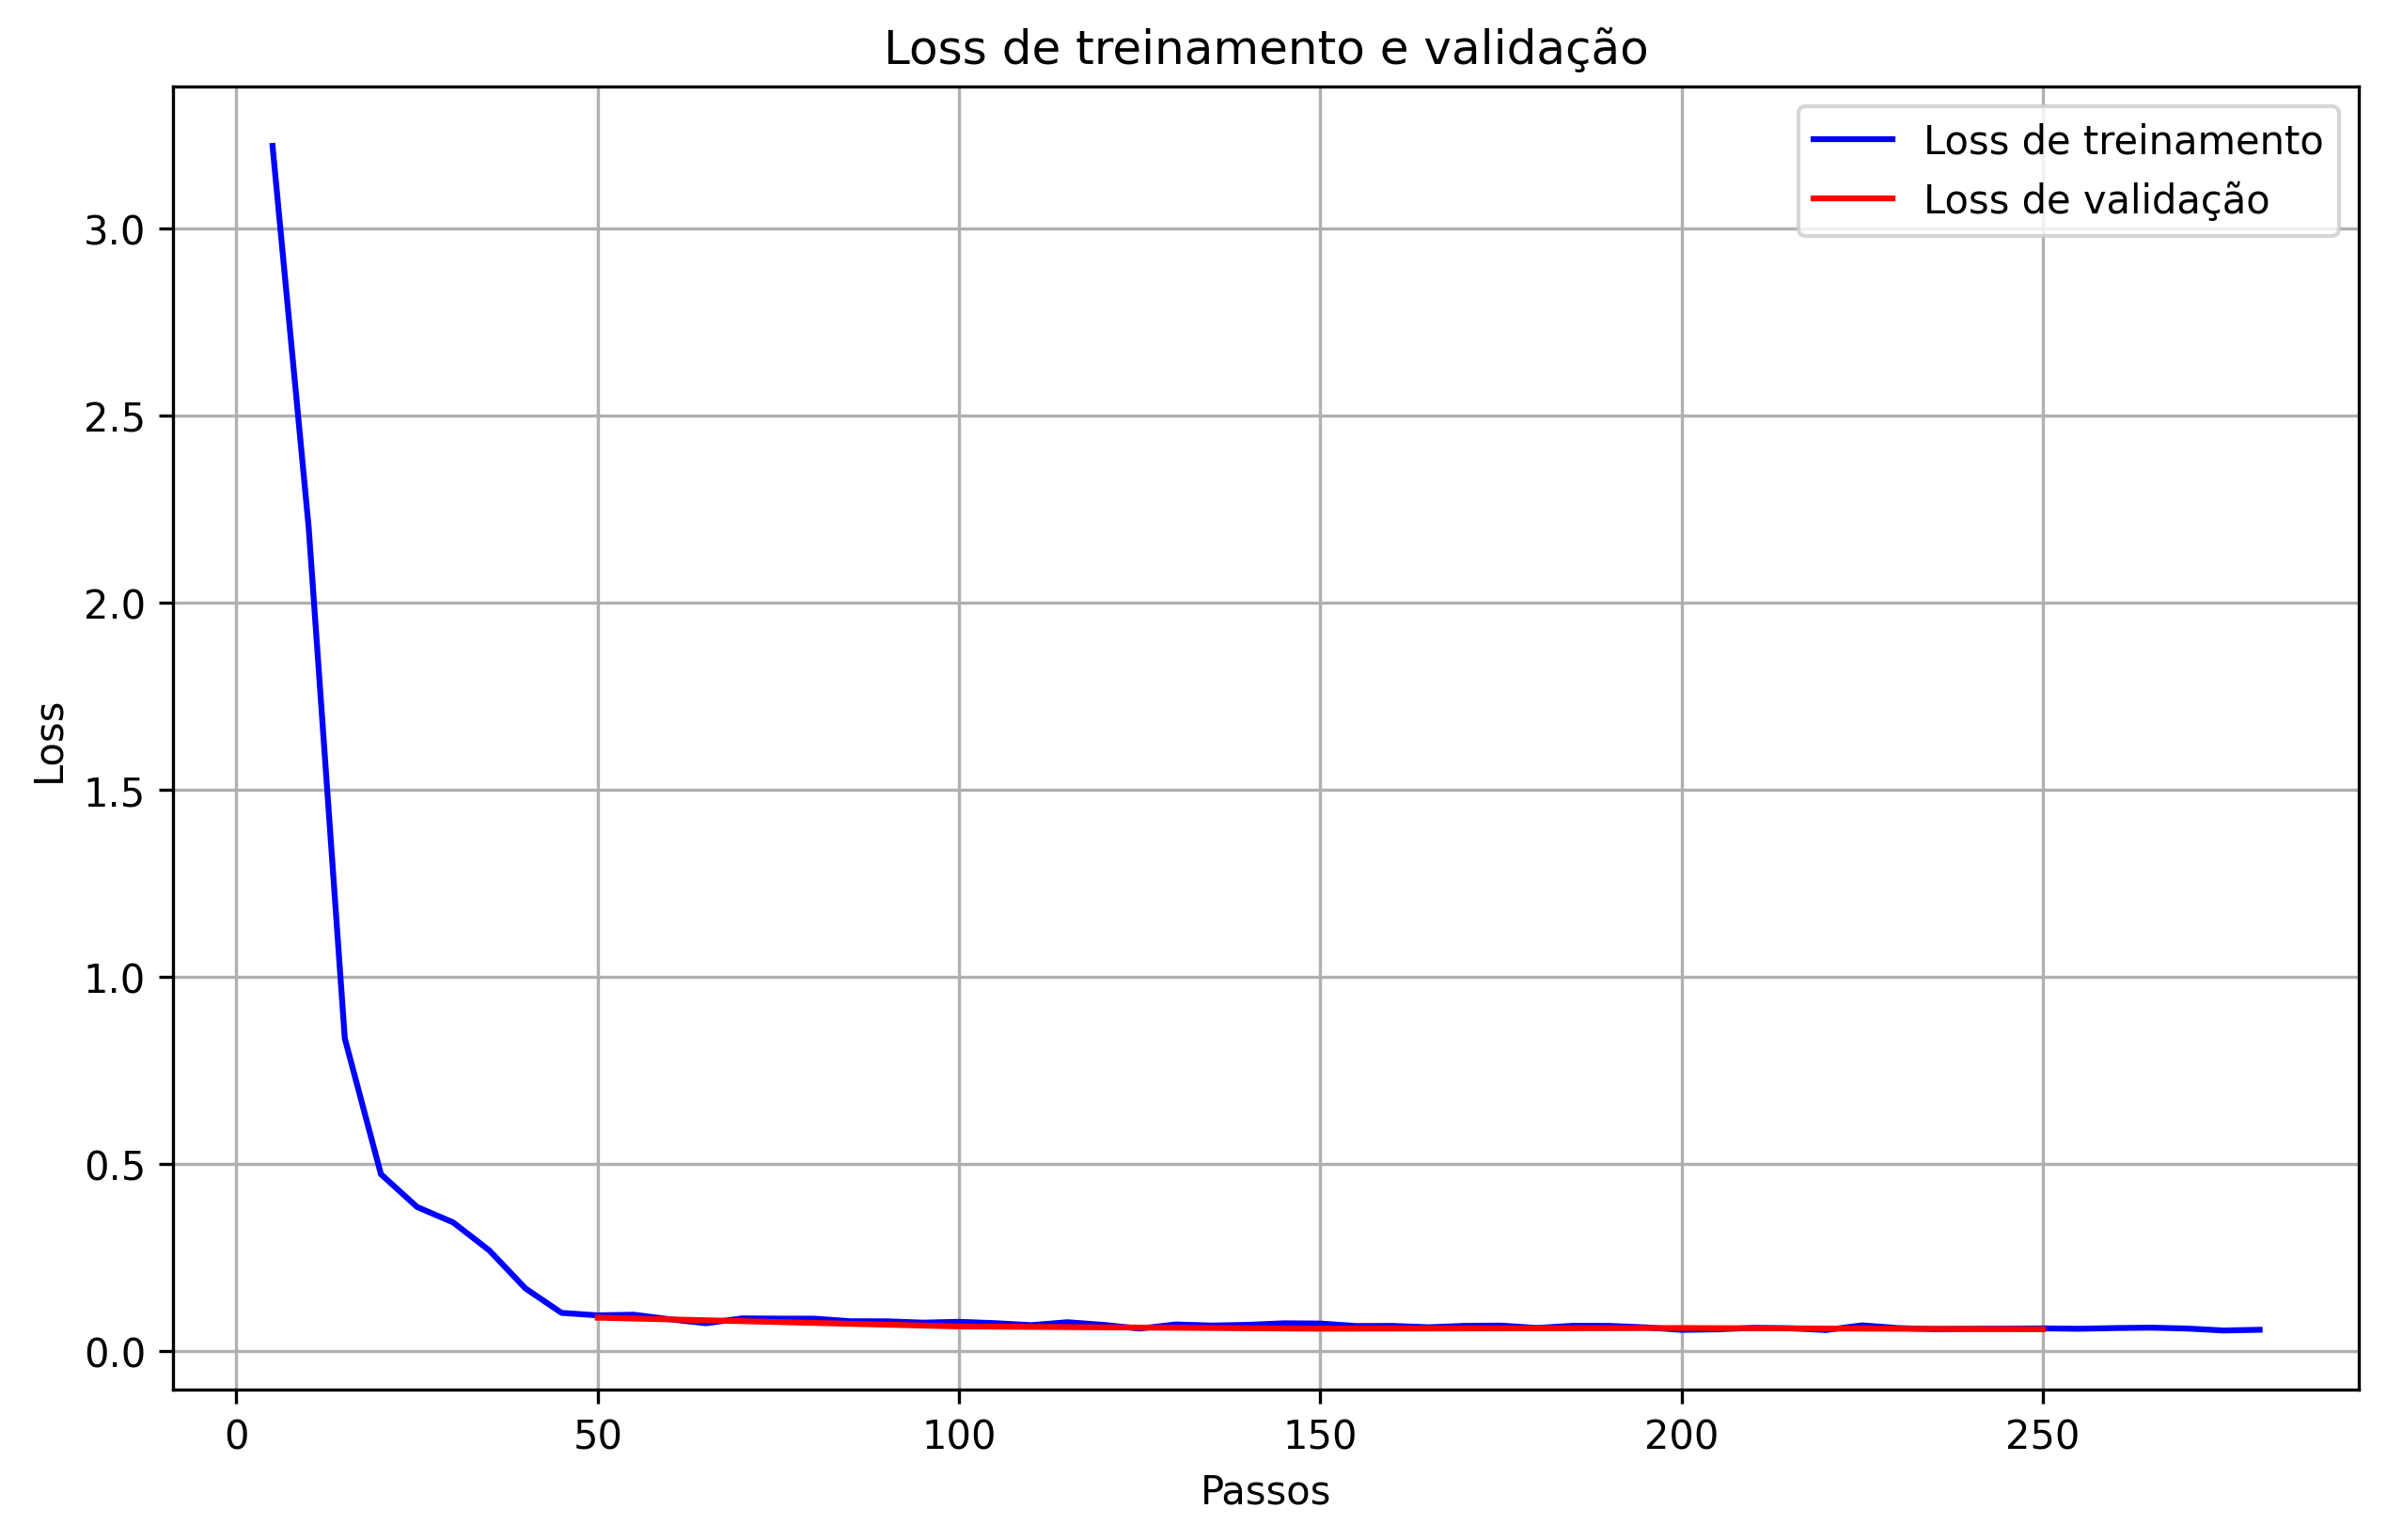
\includegraphics[width=0.725\columnwidth,keepaspectratio]{images/loss_lora_1000.png}
    \label{fig:loss_lora_1000}
    \fonte{Autoria própria.}
\end{figure}

Por último, foi feito um \textit{fine-tuning} com \ac{QLoRA} com 1800 amostras com os mesmos hiperparâmetros utilizados anteriormente. As informações sobre o treinamento
podem ser vistas na \autoref{tab:qlora_2000_training} e na \autoref{fig:loss_qlora_2000}.

\clearpage

\begin{table}[ht]
    \caption{\small Dados sobre o treinamento com \ac{QLoRA} com 1800 amostras.}
    \centering
    \begin{tabular}{l|c}
        \hline
                                    & Valor     \\ \hline
        Parâmetros treináveis       & 134348800 \\
        Tempo de treinamento (min)  & 90,77     \\
        Passos                      & 450       \\
        Memória máxima alocada (GB) & 18,744    \\ \hline
    \end{tabular}
    \label{tab:qlora_2000_training}
    \fonte{Autoria própria}
\end{table}

\begin{figure}[ht]
    \centering
    \caption{\small \textit{Loss} de treinamento e validação para o \ac{QLoRA} com 1800 amostras.}
    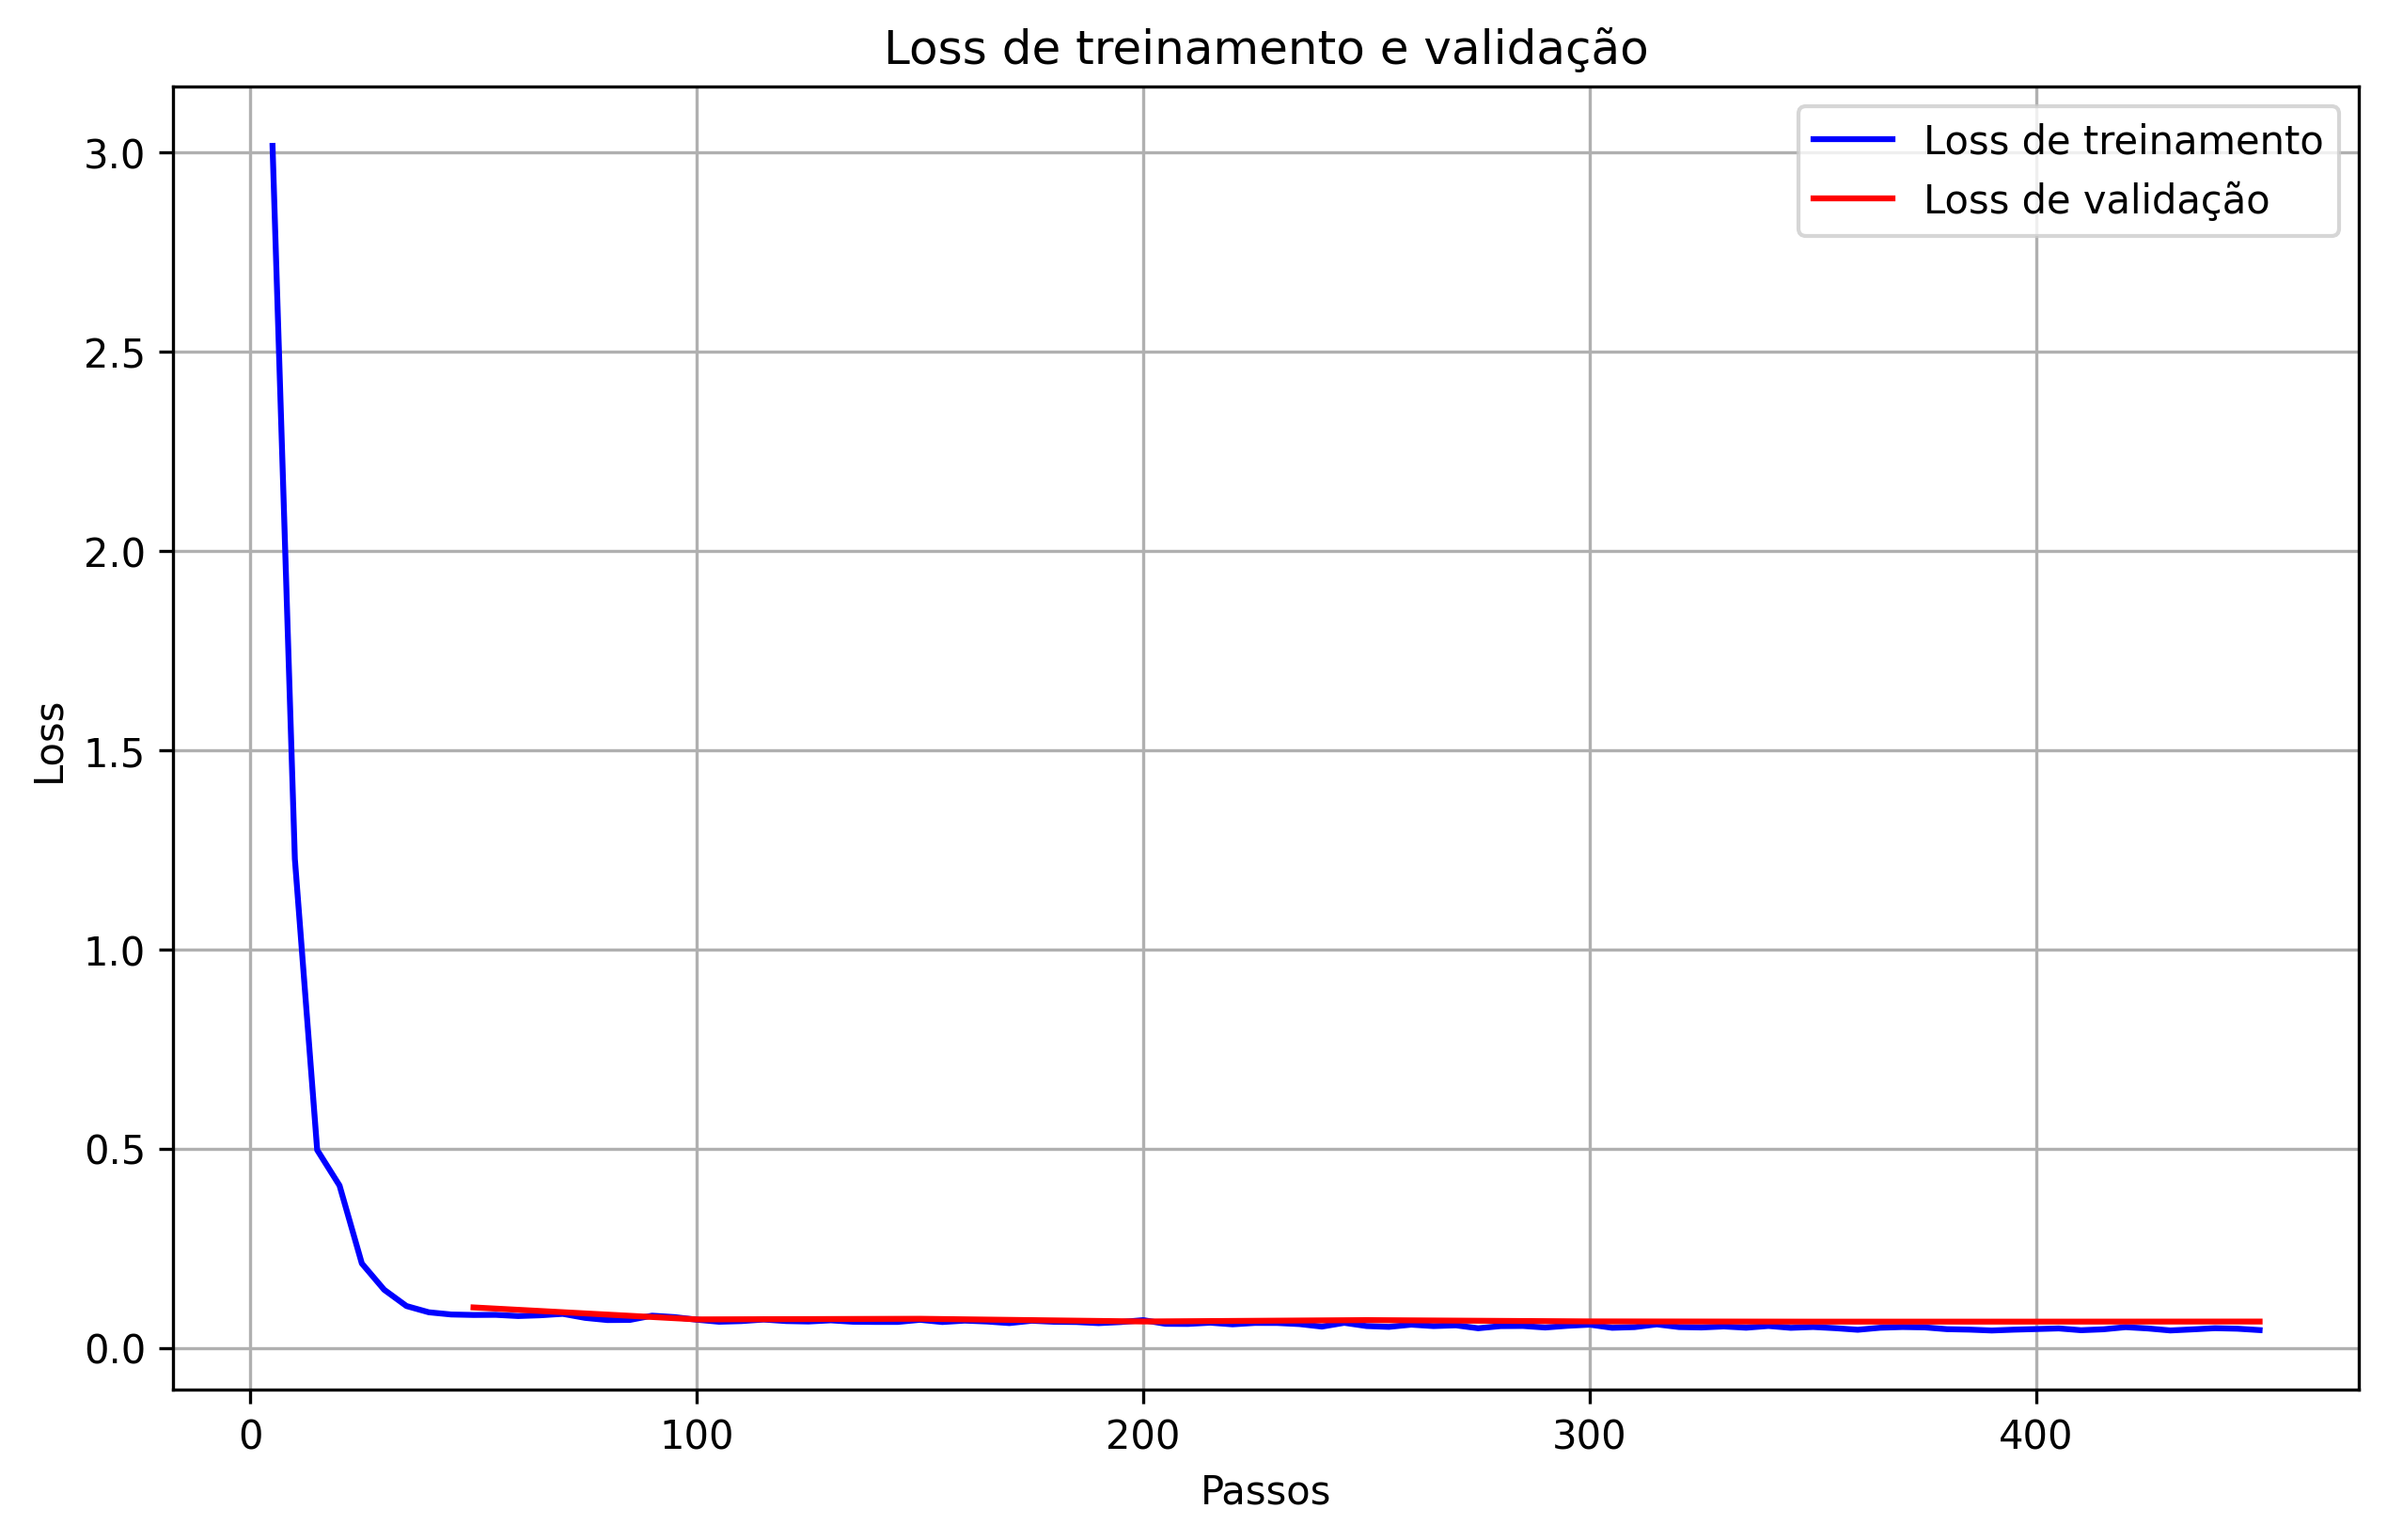
\includegraphics[width=0.725\columnwidth,keepaspectratio]{images/loss_qlora_2000.png}
    \label{fig:loss_qlora_2000}
    \fonte{Autoria própria.}
\end{figure}

\subsection{\textit{Fine-tuning} com 5000 e 9500 amostras}

Para avaliar o impacto de diferentes hiperparâmetros, foram feitos \textit{fine-tunings} modificados com 5000 e 9500 amostras. As configurações na
\autoref{tab:qlora_5000_config} se referem tanto ao \ac{QLoRA} quanto ao \ac{LoRA}. Foi utilizado somente o \ac{QLoRA} no treinamento com 9500 amostras. Os dados dos
treinamentos podem ser conferidos na \autoref{tab:qlora_5000_training}, \autoref{tab:lora_5000_training} e \autoref{tab:qlora_9500_training}, enquanto o \textit{loss}
pode ser conferido na \autoref{fig:loss_qlora_5000}, \autoref{fig:loss_lora_5000} e \autoref{fig:loss_qlora_9500}.

\clearpage

\begin{table}[ht]
    \caption{\small Hiperparâmetros para o \textit{fine-tuning} com 5000 e 9500 amostras. A primeira seção se refere às configurações específicas de \ac{PEFT}, enquanto
        a segunda se refere ao treinamento em geral.}
    \centering
    \begin{tabular}{l|c}
        \hline
        Hiperparâmetro                             & Valor                                  \\ \hline
        Camadas e módulos treinados                & Visão, linguagem, atenção e \ac{MLP}   \\
        Rank                                       & 64                                     \\
        Alfa (\begin{math}\alpha_{LoRA}\end{math}) & 64                                     \\
        Dropout                                    & 0,05                                   \\
        \ac{rsLoRA}                                & Sim                                    \\ \hline
        Taxa de aprendizado                        & \begin{math}1 \times 10^{-4}\end{math} \\
        Razão de aquecimento                       & 0                                      \\
        Tipo de escalonador da taxa de aprendizado & Constante                              \\
        Decaimento de peso                         & 0,01                                   \\
        Épocas                                     & 3                                      \\
        Passos a cada validação                    & A cada 5\% dos passos                  \\
        Otimizador                                 & \ac{Adam} paginado de 32 bits          \\
        Tipo numérico                              & \ac{BF16}                              \\ \hline
    \end{tabular}
    \label{tab:qlora_5000_config}
    \fonte{Autoria própria}
\end{table}

\begin{table}[ht]
    \caption{\small Dados sobre o treinamento com \ac{QLoRA} com 5000 amostras.}
    \centering
    \begin{tabular}{l|c}
        \hline
                                    & Valor     \\ \hline
        Parâmetros treináveis       & 268697600 \\
        Tempo de treinamento (min)  & 96,63     \\
        Passos                      & 1875      \\
        Memória máxima alocada (GB) & 18,967    \\ \hline
    \end{tabular}
    \label{tab:qlora_5000_training}
    \fonte{Autoria própria}
\end{table}

\begin{table}[ht]
    \caption{\small Dados sobre o treinamento com \ac{LoRA} com 5000 amostras.}
    \centering
    \begin{tabular}{l|c}
        \hline
                                    & Valor     \\ \hline
        Parâmetros treináveis       & 268697600 \\
        Tempo de treinamento (min)  & 100,33    \\
        Passos                      & 1875      \\
        Memória máxima alocada (GB) & 31,48     \\ \hline
    \end{tabular}
    \label{tab:lora_5000_training}
    \fonte{Autoria própria}
\end{table}

\clearpage

\begin{table}[ht]
    \caption{\small Dados sobre o treinamento com \ac{QLoRA} com 9500 amostras.}
    \centering
    \begin{tabular}{l|c}
        \hline
                                    & Valor     \\ \hline
        Parâmetros treináveis       & 268697600 \\
        Tempo de treinamento (min)  & 177,44    \\
        Passos                      & 3564      \\
        Memória máxima alocada (GB) & 18,971    \\ \hline
    \end{tabular}
    \label{tab:qlora_9500_training}
    \fonte{Autoria própria}
\end{table}

\begin{figure}[ht]
    \centering
    \caption{\small \textit{Loss} de treinamento e validação para o \ac{QLoRA} com 5000 amostras.}
    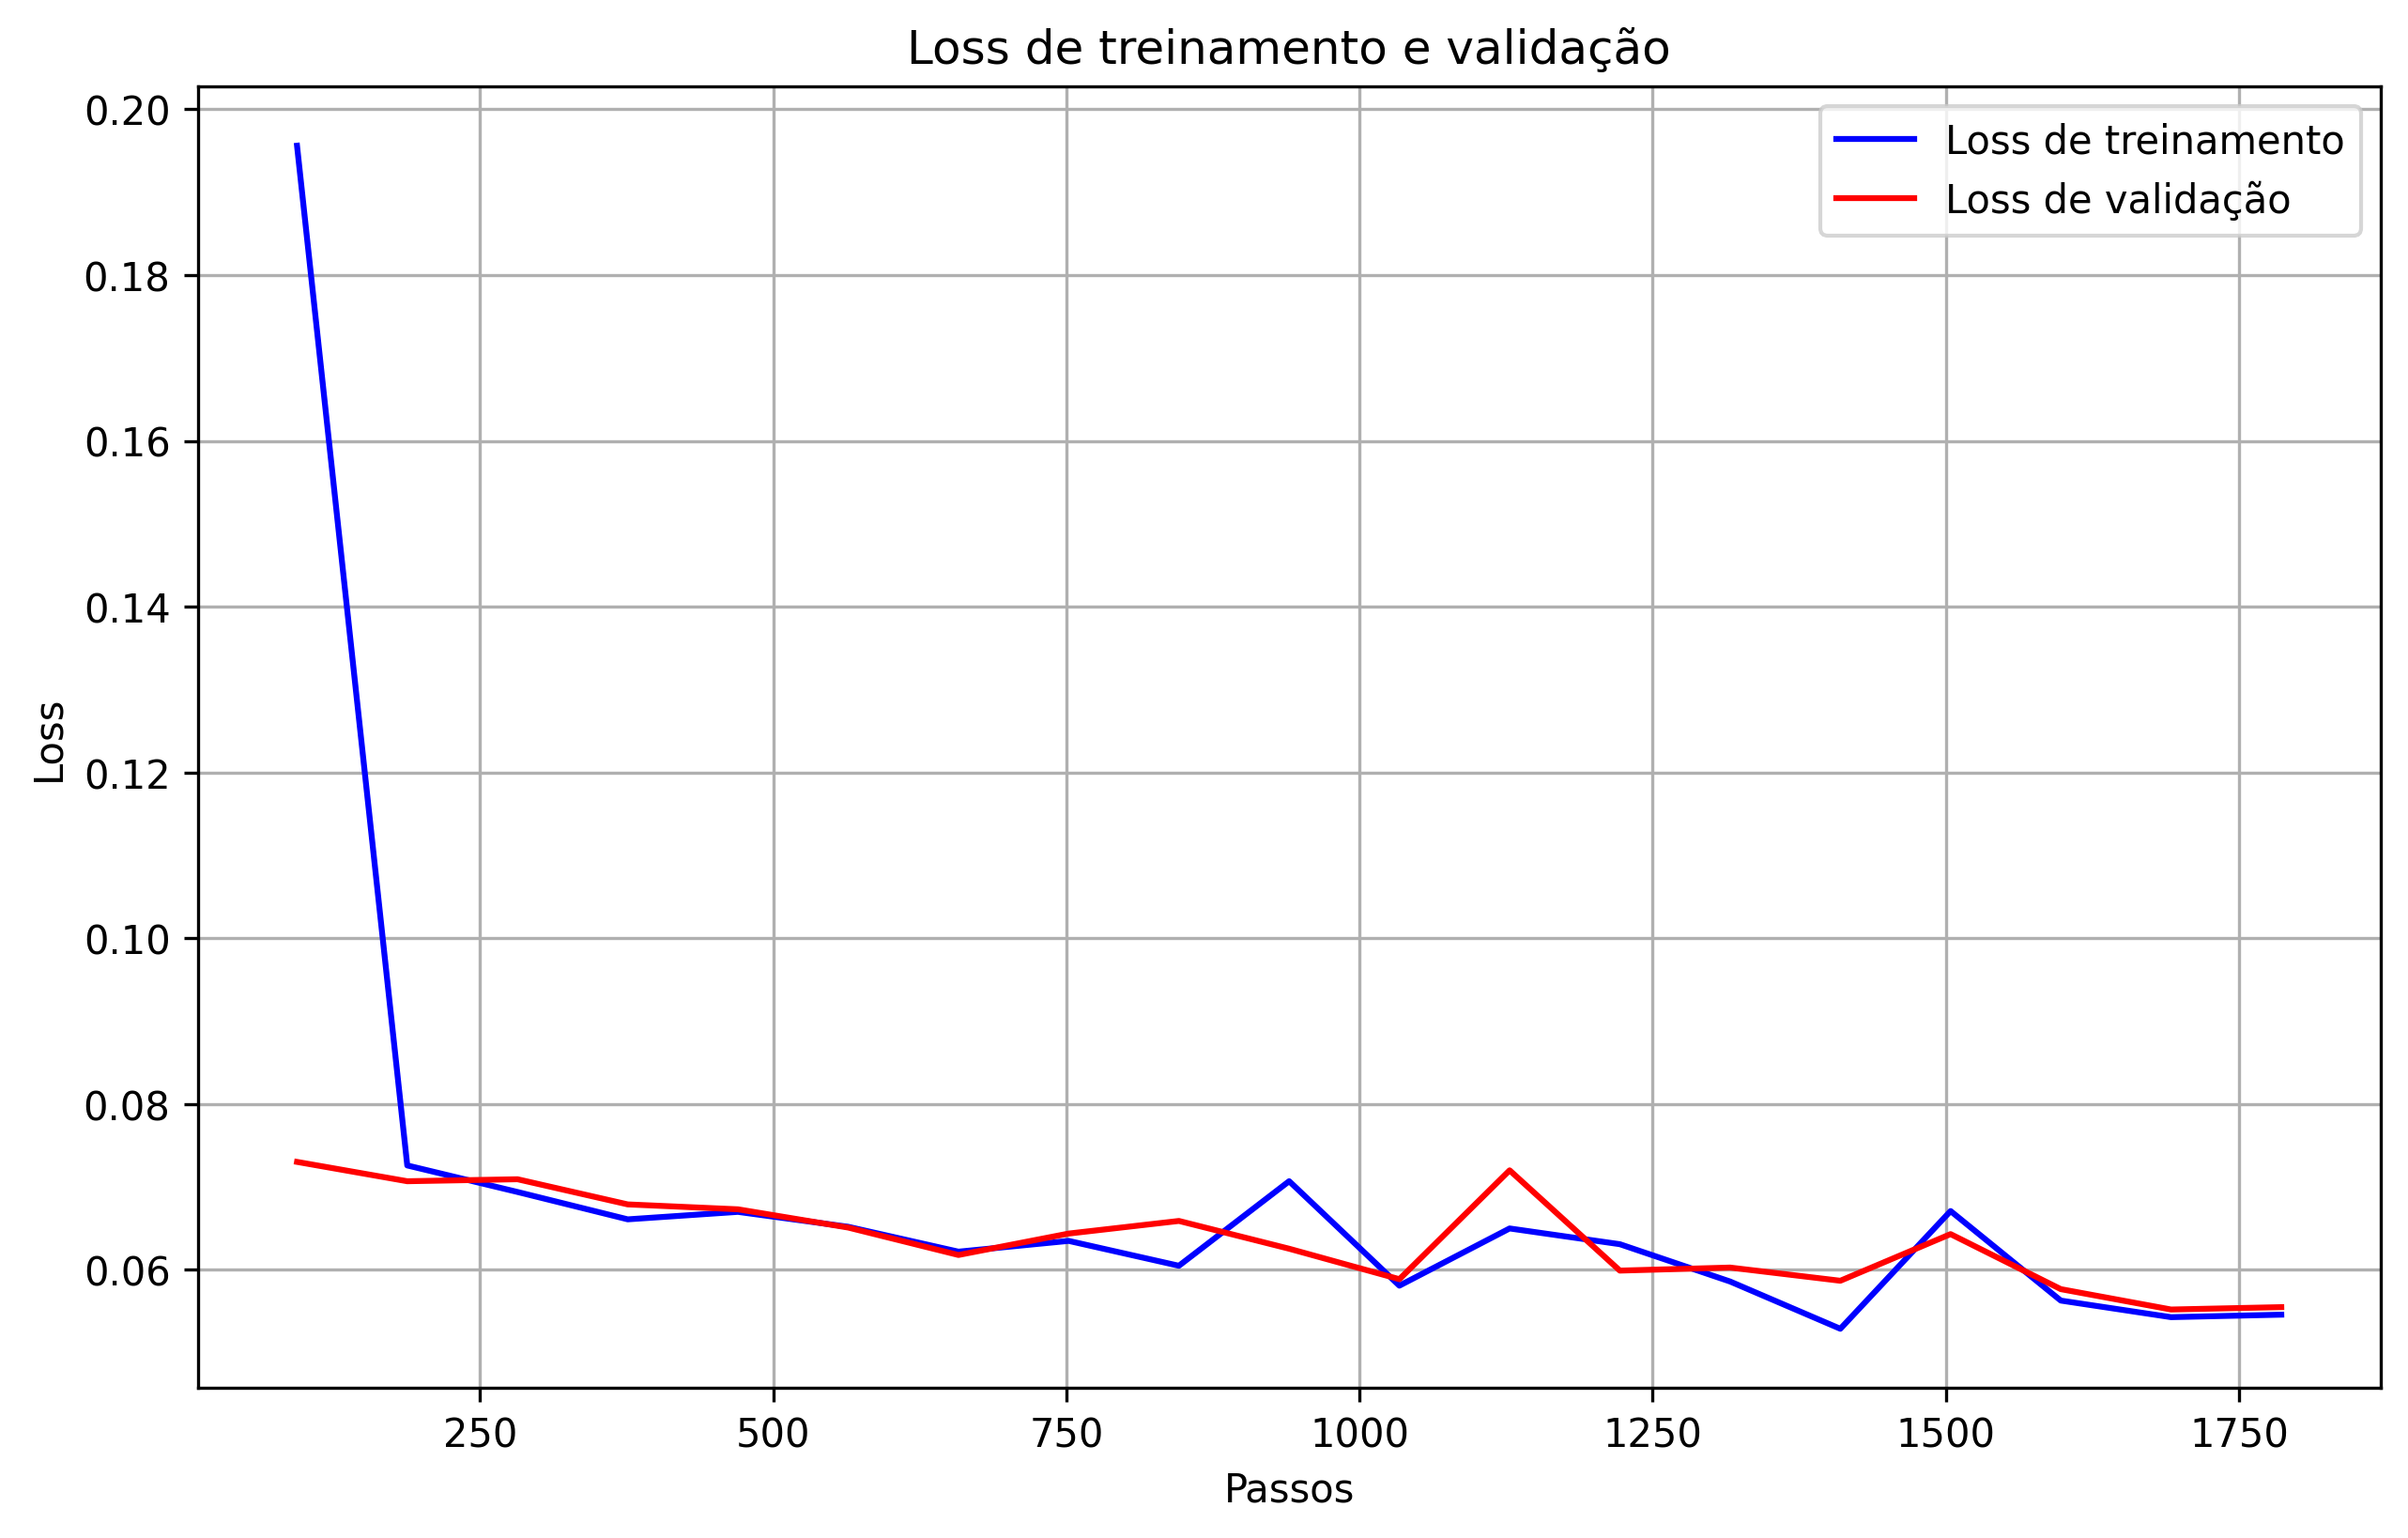
\includegraphics[width=0.725\columnwidth,keepaspectratio]{images/loss_qlora_5000.png}
    \label{fig:loss_qlora_5000}
    \fonte{Autoria própria.}
\end{figure}

\clearpage

\begin{figure}[ht]
    \centering
    \caption{\small \textit{Loss} de treinamento e validação para o \ac{LoRA} com 5000 amostras.}
    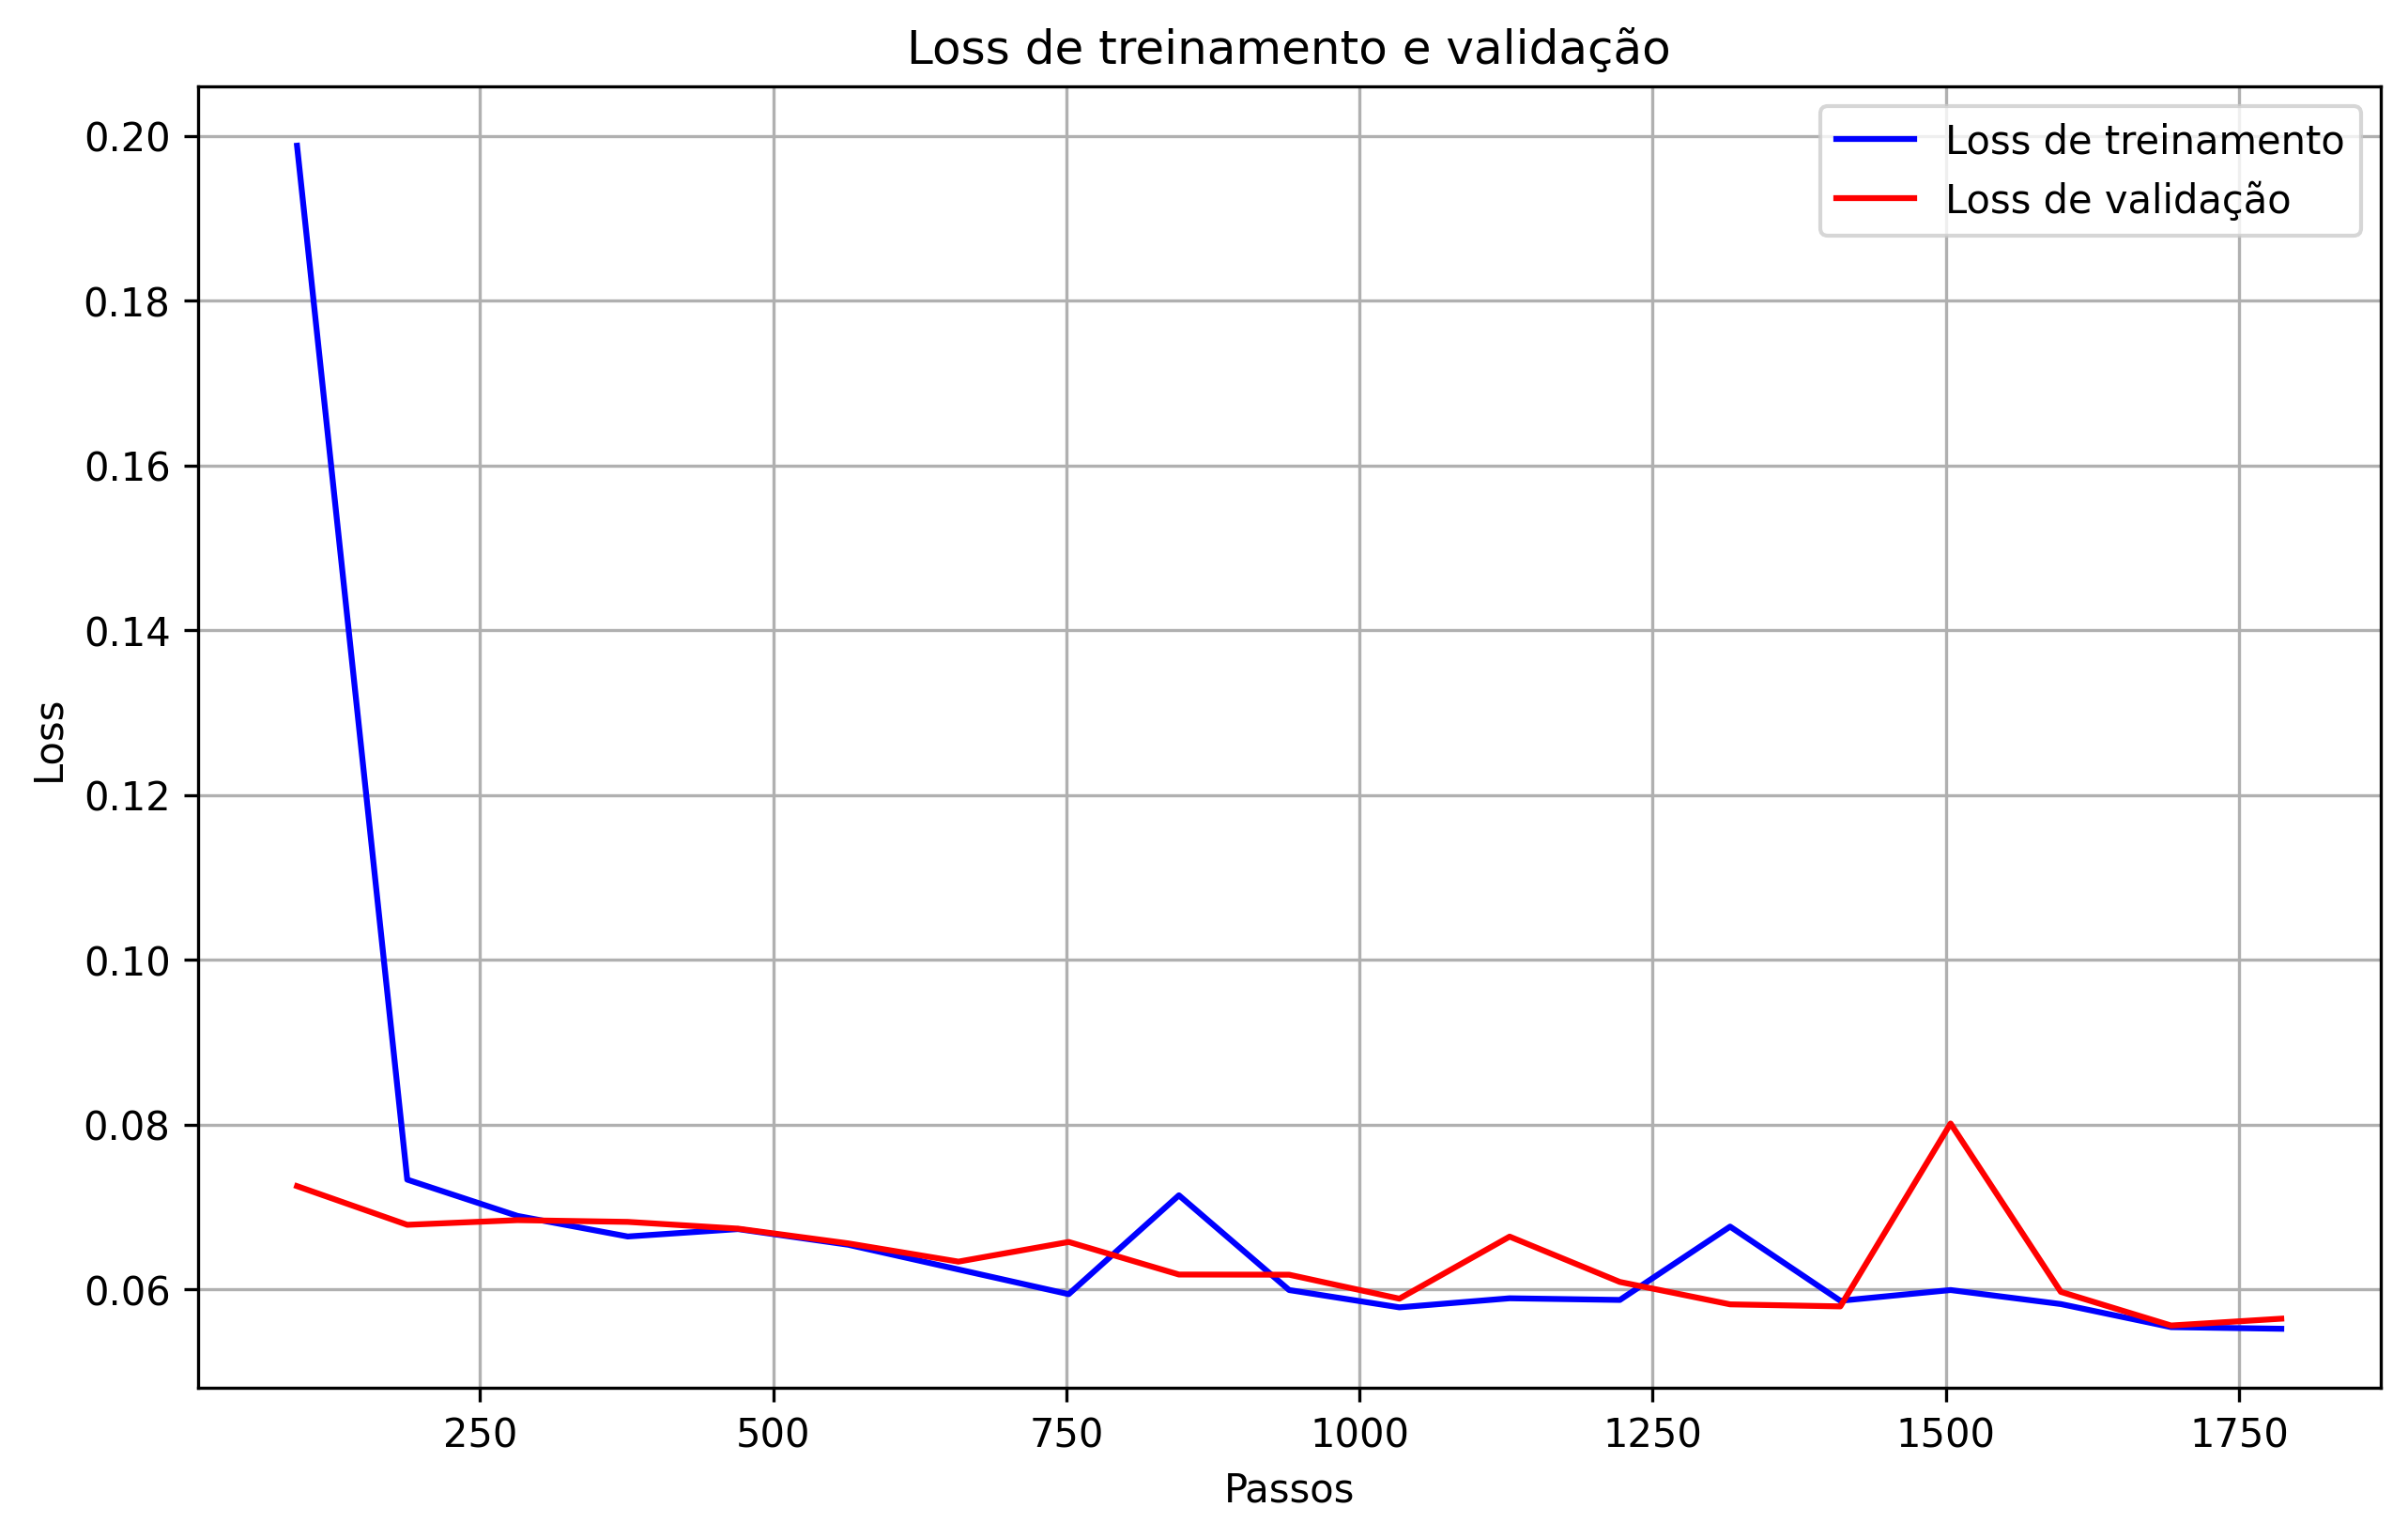
\includegraphics[width=0.725\columnwidth,keepaspectratio]{images/loss_lora_5000.png}
    \label{fig:loss_lora_5000}
    \fonte{Autoria própria.}
\end{figure}

\begin{figure}[ht]
    \centering
    \caption{\small \textit{Loss} de treinamento e validação para o \ac{QLoRA} com 9500 amostras.}
    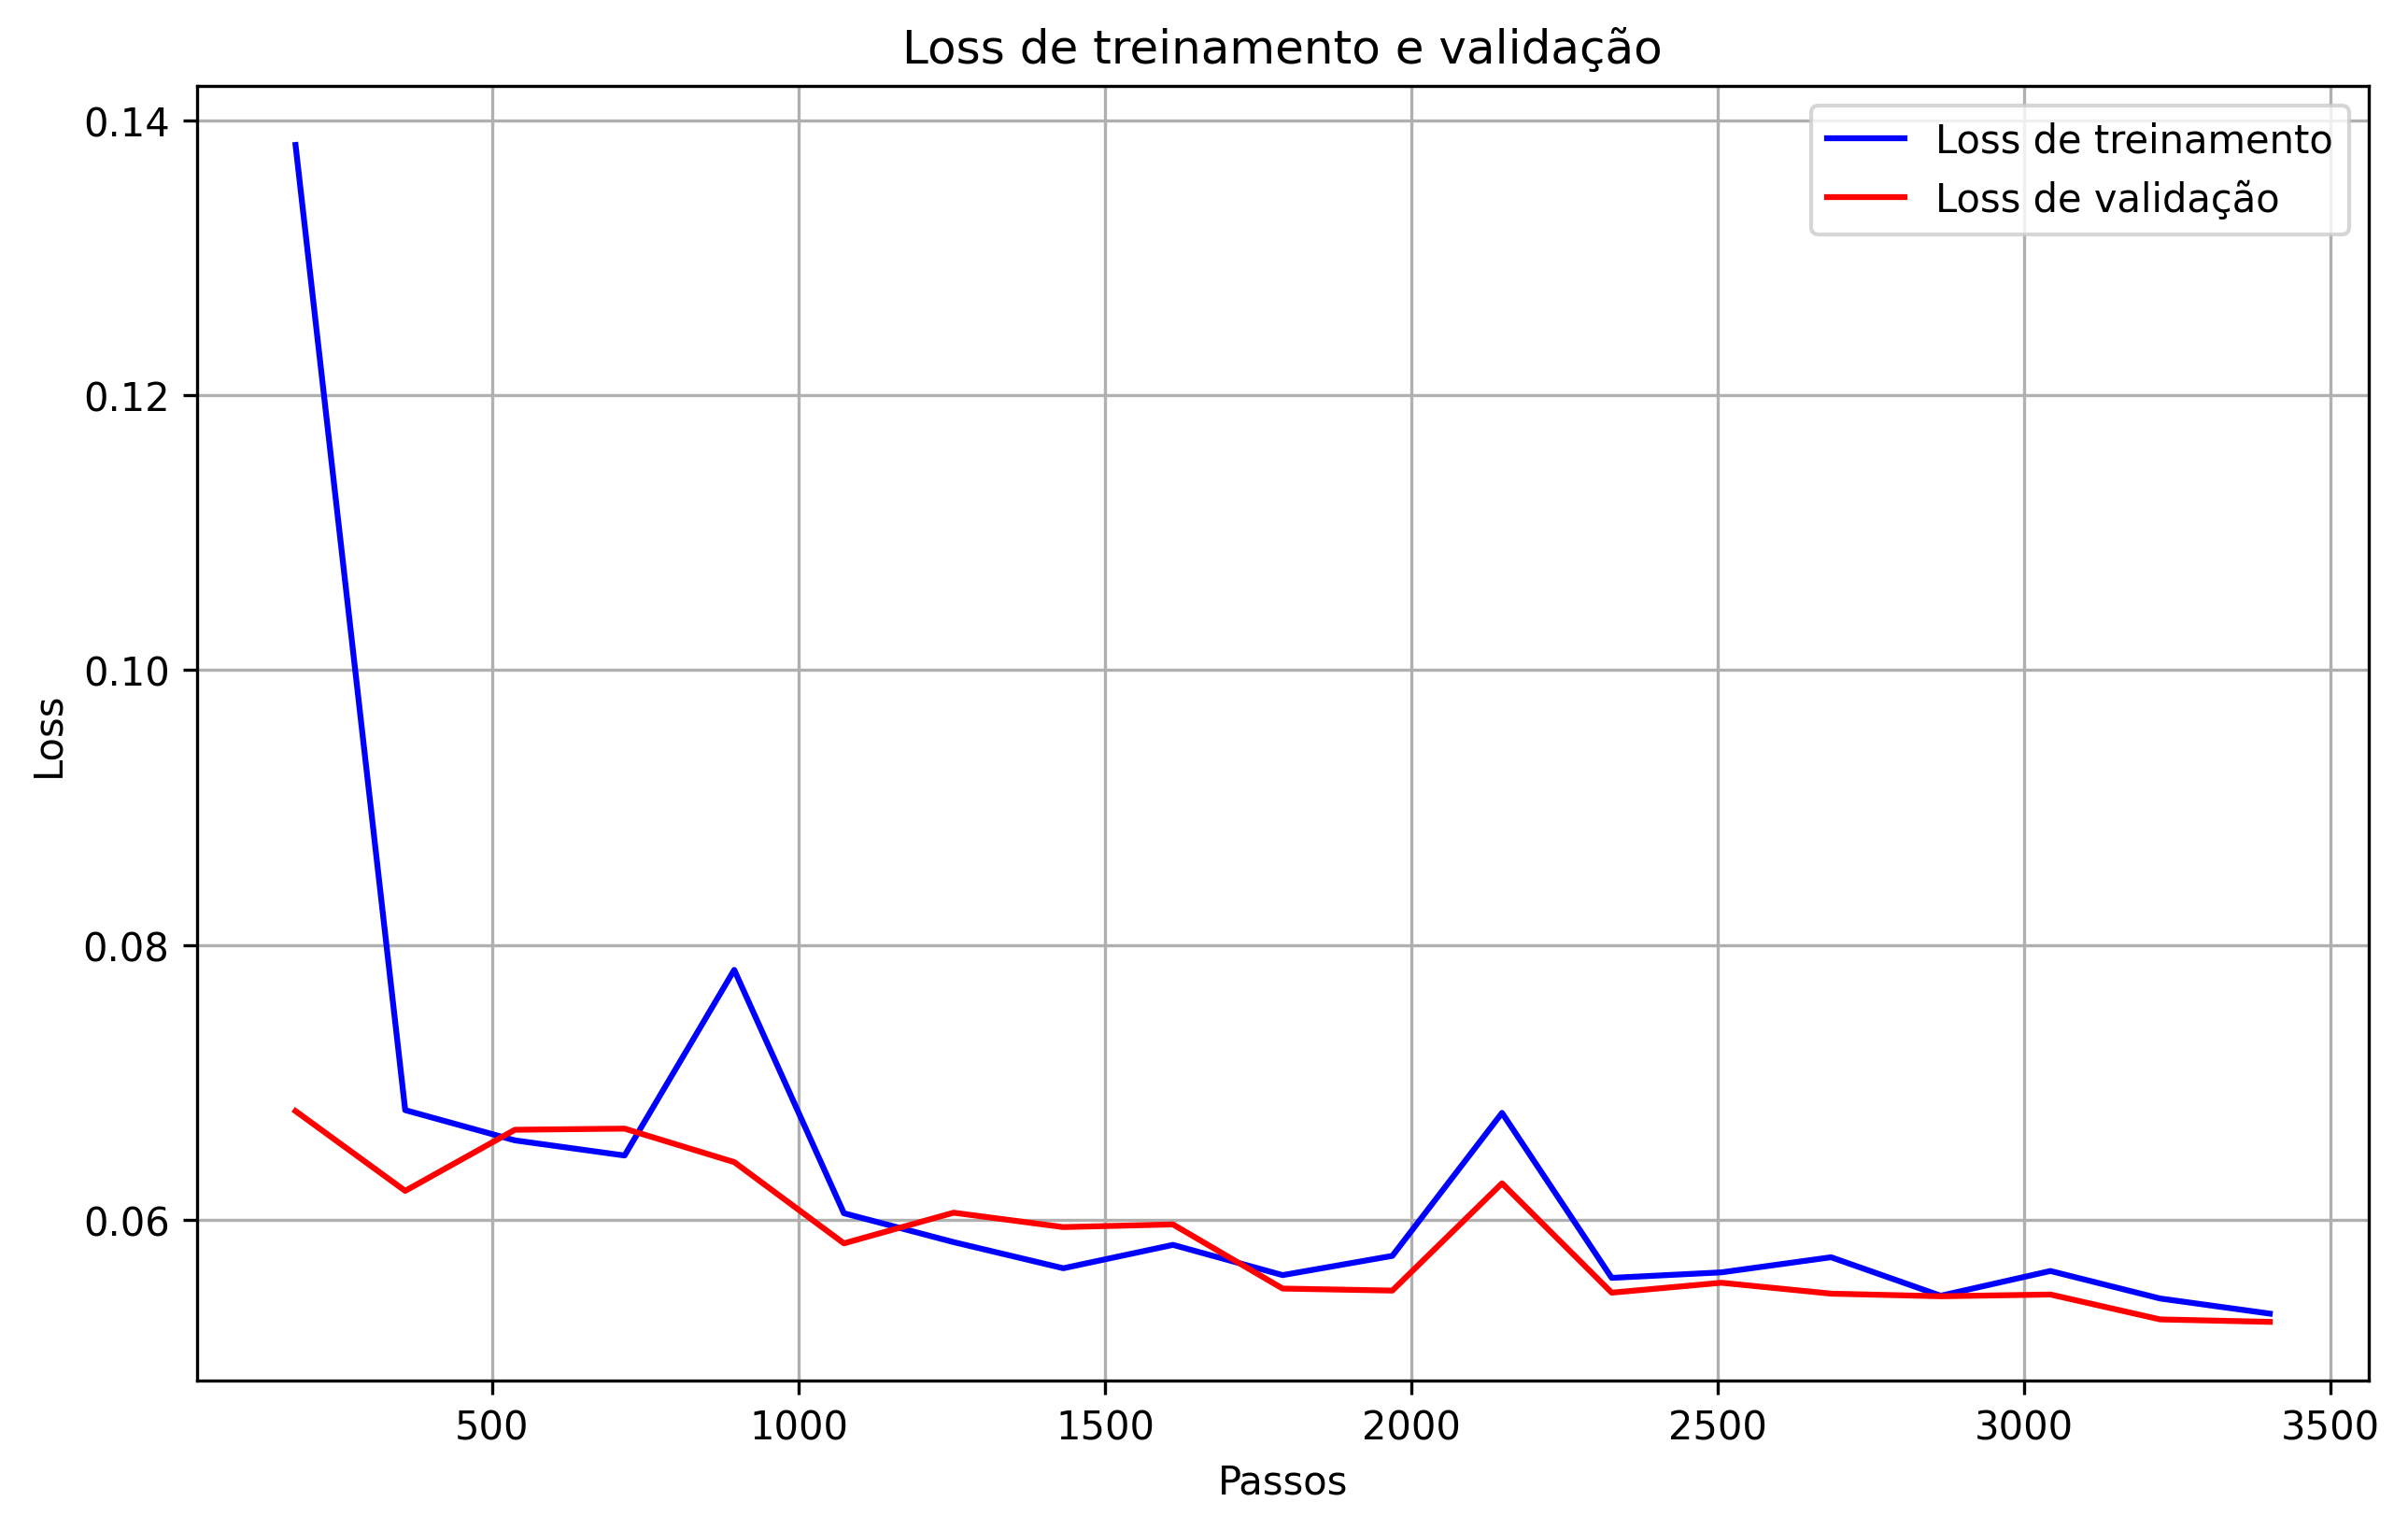
\includegraphics[width=0.725\columnwidth,keepaspectratio]{images/loss_qlora_9500.png}
    \label{fig:loss_qlora_9500}
    \fonte{Autoria própria.}
\end{figure}

\subsection{Análise dos treinamentos}

A vantagem no baixo gasto de memória do \ac{QLoRA} se torna evidente com os treinamentos, usando em média 1,8 vezes menos memória que o \ac{LoRA}. Observa-se também
que as configurações de \textit{fine-tuning} usadas no treinamento com 5000 e 9500 amostras levaram a uma maior instabilidade no \textit{loss} do longo dos passos.

\section{Testes}

Os testes se consistiram em uma série de perguntas aos modelos, em que foram usadas duas modalidades de pergunta, uma livre e outra objetiva. Na pergunta livre o
\textit{prompt} é definido como:

\begin{dialogue}
    \speak{Usuário} \textit{Classify the skin lesion in the image. \textbf{<imagem>}}
\end{dialogue}

Já na pergunta objetiva, é esperado que o modelo informe apenas o nome da doença com base nas opções possíveis do conjunto de dados, sendo que o \textit{prompt} usado é:

\begin{dialogue}
    \speak{Usuário} \textit{Classify the skin lesion in the image. Say only the name of the disease and nothing else. The diseases to be classified are: melanocytic Nevi,
        melanoma, benign keratosis-like lesions, basal cell carcinoma, actinic keratoses, vascular lesions and dermatofibroma.\textbf{<imagem>}}
\end{dialogue}

Foram feitas 100 perguntas livres e 1000 perguntas objetivass para cada modelo treinado e para o \ac{LLaMA}-3.2-11B-Vision-Instruct na versão normal e na quantizada. As
imagens utilizadas vieram da seção de teste do conjunto de dados. A \textit{temperatura}, uma variável que define a previsibilidade do modelo, foi definida como 0,1
para que as respostas fossem mais precisas. Além disso, o número máximo de \textit{tokens} foi definido como 128.

\section{Análise dos resultados parciais}

Os testes com perguntas livres foram avaliados manualmente para observar o formato de resposta dos modelos, enquanto os testes com perguntas objetivas foram processados
para a extração das lesões previstas para as imagens. Com esses dados, foram geradas matrizes de confusão com os cálculos da acurácia de cada modelo.

\subsection{Análise do LLaMA-3.2-Vision-Instruct}

Tanto o modelo na versão normal quanto o modelo quantizado apresentaram respostas bem variadas para cada pergunta livre. Em geral, as respostas apresentam uma estrutura
de passos que se baseia em metodologias de classificação de lesões de pele. O diálogo abaixo apresenta uma classificação correta para a imagem de um melanoma:

\begin{dialogue}
    \speak{Usuário} \textit{Classify the skin lesion in the image. \textbf{<imagem de um melanoma>}} \\
    \speak{Modelo} \textit{\textbf{Step 1: Identify the lesion.} \\
        The image shows a skin lesion with an irregular border and a dark brown color. \\
        \textbf{Step 2: Determine the characteristics of the lesion.} \\
        The lesion has an irregular border, which is a characteristic of melanoma. The dark brown color is also consistent with melanoma. \\
        \textbf{Step 3: Consider the possible diagnoses.} \\
        Based on the characteristics of the lesion, it is likely that the diagnosis is melanoma. \\
        \textbf{Step 4: Provide the final answer.} \\
        \textbf{Answer:} Melanoma}
\end{dialogue}

Muitas respostas apresentaram uma classificação incorreta, embora tenham sido descritivas sobre a lesão. No exemplo abaixo, o modelo classificou um nevo melanocítico
como um melanoma:

\begin{dialogue}
    \speak{Usuário} \textit{Classify the skin lesion in the image. \textbf{<imagem de um nevo melanocítico>}} \\
    \speak{Modelo} \textit{\textbf{Step 1: Identify the lesion} \\
        The image shows a brown, irregularly shaped lesion with a darker brown border. \\
        \textbf{Step 2: Determine the characteristics of the lesion} \\
        The lesion is asymmetrical, has an irregular border, and has multiple colors. \\
        \textbf{Step 3: Classify the lesion} \\
        Based on the characteristics of the lesion, it is classified as a melanoma. \\
        \textbf{Answer:} Melanoma}
\end{dialogue}

Algumas respostas não apresentaram uma classificação precisa, sendo que o modelo informou apenas que a imagem se tratava de uma lesão de pele. Um exemplo assim pode ser
visto no diálogo abaixo:

\begin{dialogue}
    \speak{Usuário} \textit{Classify the skin lesion in the image. \textbf{<imagem de um nevo melanocítico>}} \\
    \speak{Modelo} \textit{The skin lesion in the image appears to be a dermatological condition, likely a typeof skin cancer or a benign growth. However, without
        further information or a medical diagnosis, it is difficult to provide a definitive classification.}
\end{dialogue}

Já nas respostas às perguntas objetivas, o modelo quantizado teve um desempenho levemente pior em relação ao não quantizado. Porém, ambos tiveram um desempenho pouco
satisfatório, a versão quantizada atingiu apenas 11,8\% de acurácia e a não quantizada atingiu 14\%.

A \autoref{fig:confusion_matrix_llama_quantized} e a \autoref{fig:confusion_matrix_llama} apresentam as matrizes de confusão normalizadas pelos valores verdadeiros para
o modelo quantizado e o não quantizado, respectivamente. Nota-se que eles classificaram as lesões como melanoma em uma escala desproporcional, o \ac{LLaMA} quantizado
classificou 97,6\% das lesões como melanoma, enquanto o não quantizado classificou 88,3\%. Também pode-se notar uma tendência da classificação de lesões vasculares como
dermatofibroma por parte do modelo não quantizado.

Foram registradas 3 respostas incertas para o modelo quantizado e apenas uma para o não quantizado.

\begin{figure}[ht]
    \centering
    \caption{\small Matriz de confusão para o \ac{LLaMA}-11B-Vision-Instruct quantizado.}
    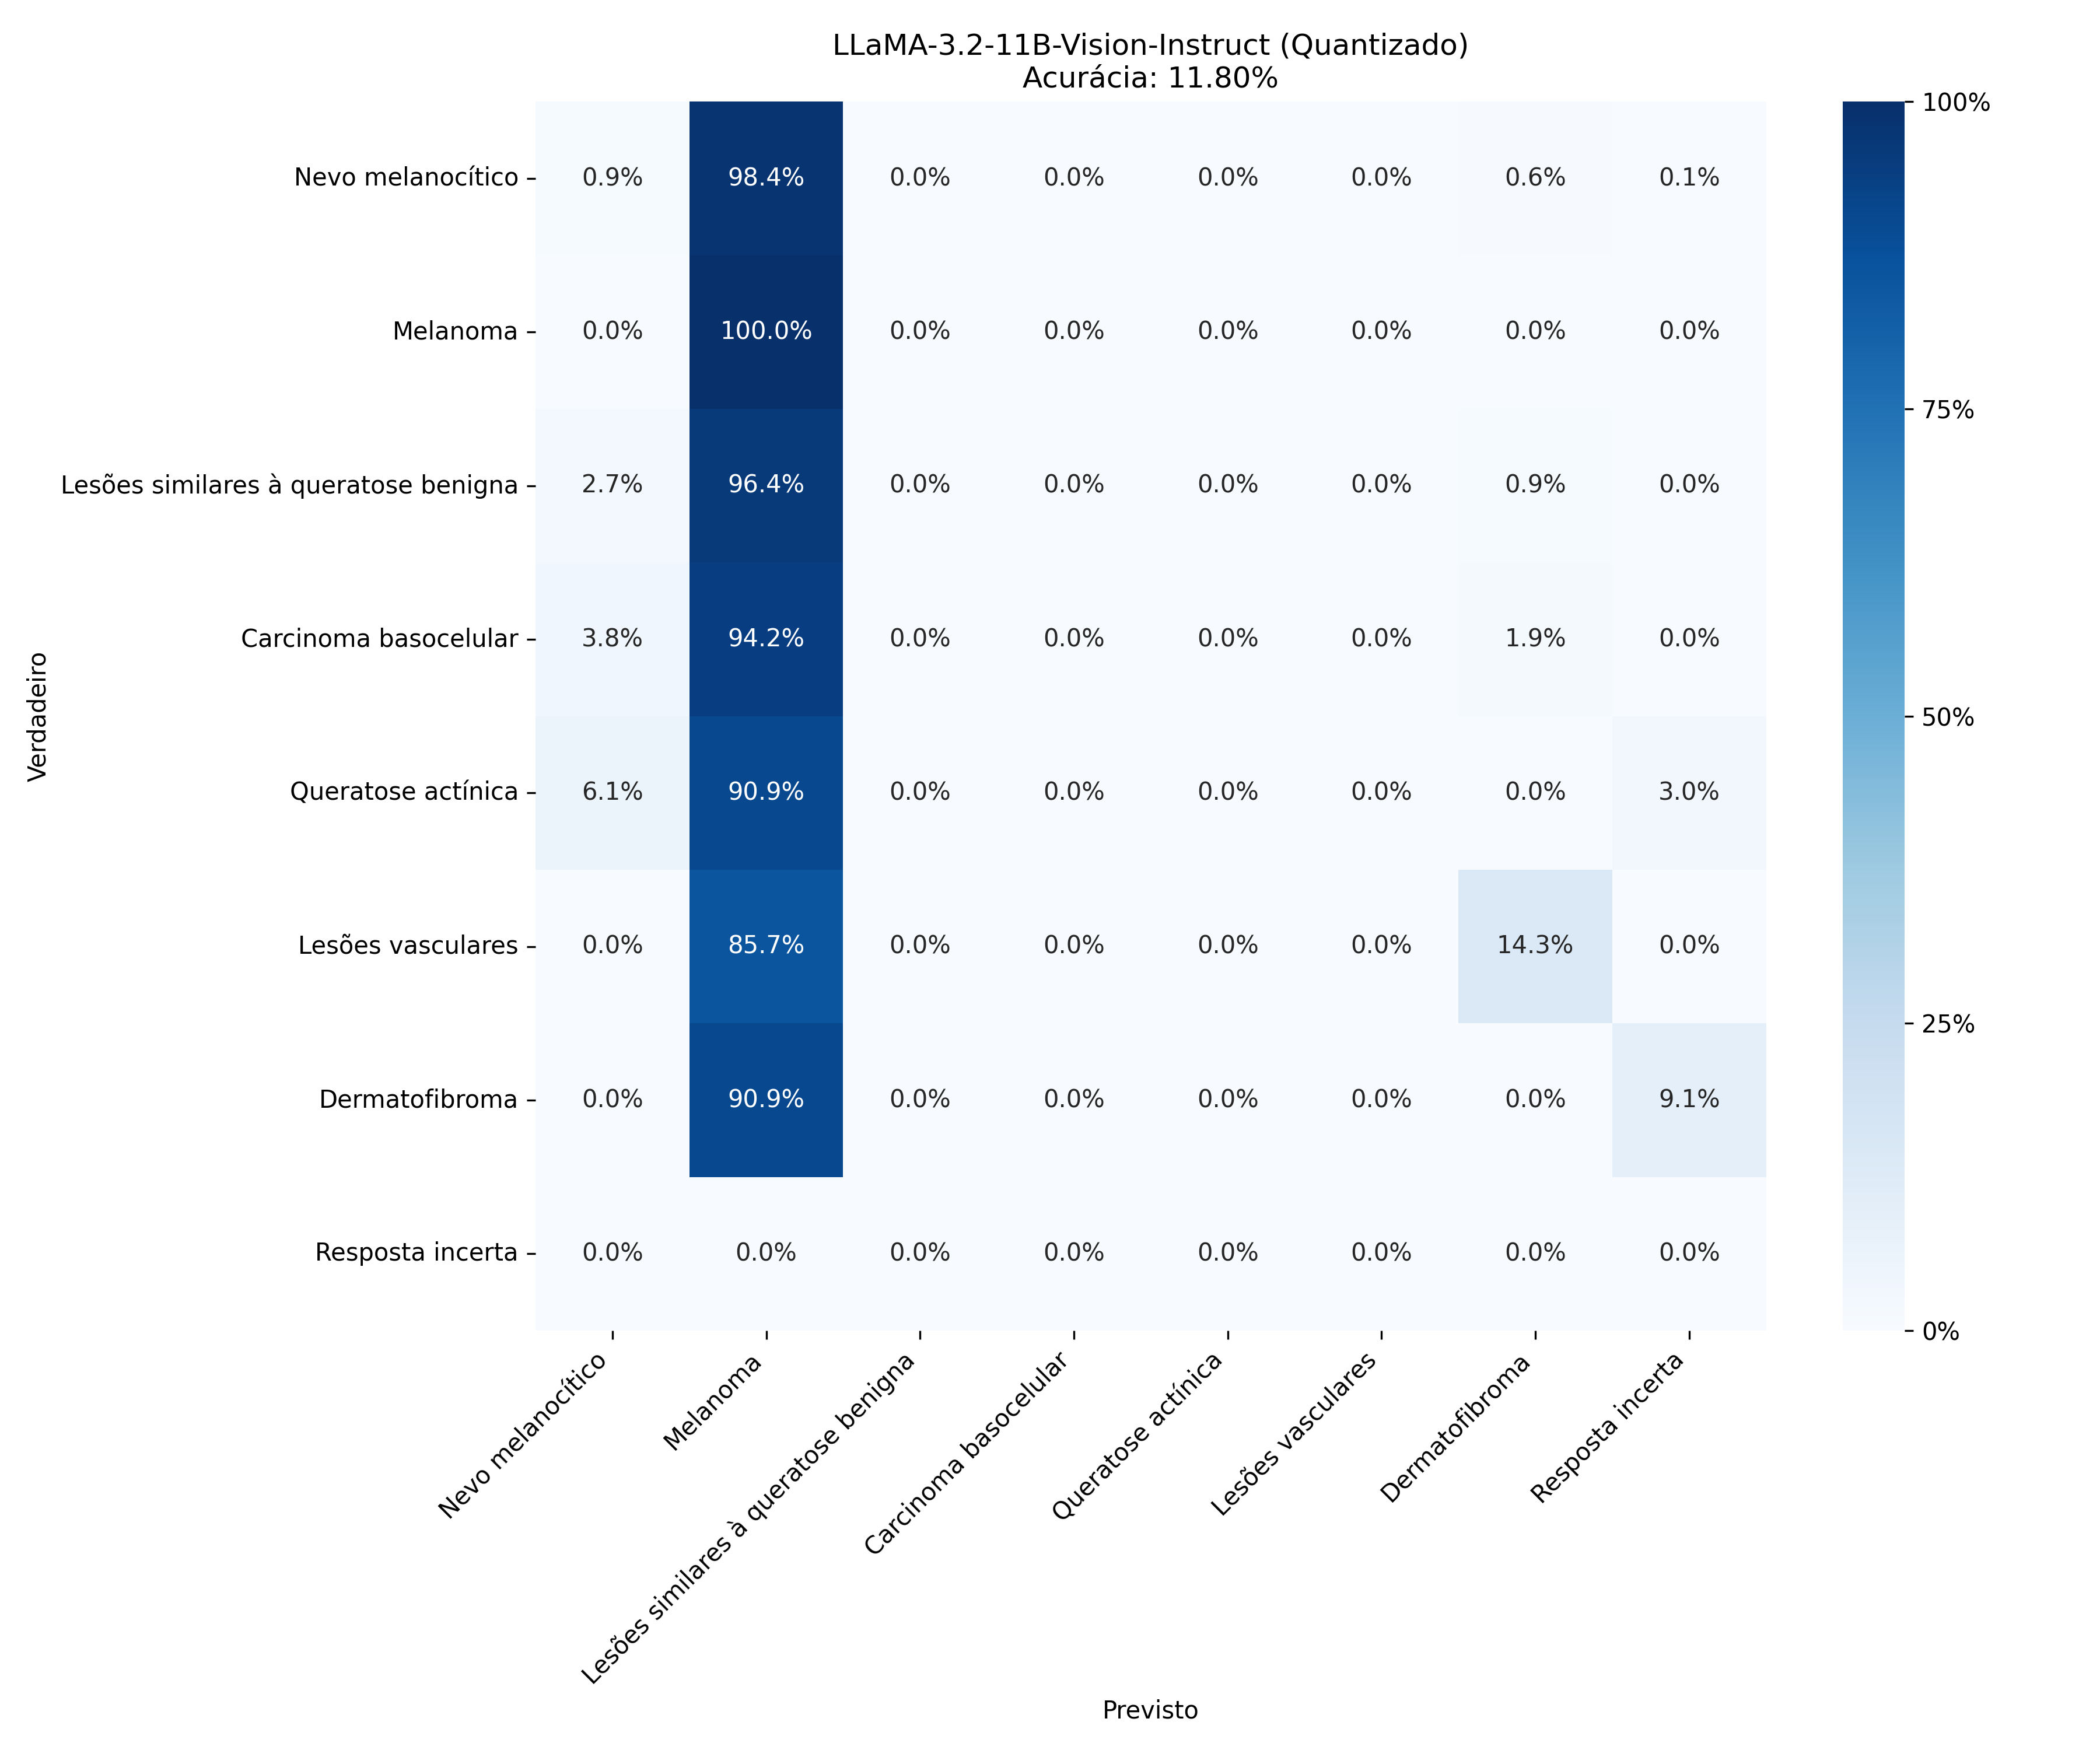
\includegraphics[width=1\columnwidth,keepaspectratio]{images/confusion_matrix_llama_3.2_11b_vision_instruct_quantized.png}
    \label{fig:confusion_matrix_llama_quantized}
    \fonte{Autoria própria.}
\end{figure}

\clearpage

\begin{figure}[ht]
    \centering
    \caption{\small Matriz de confusão para o \ac{LLaMA}-11B-Vision-Instruct.}
    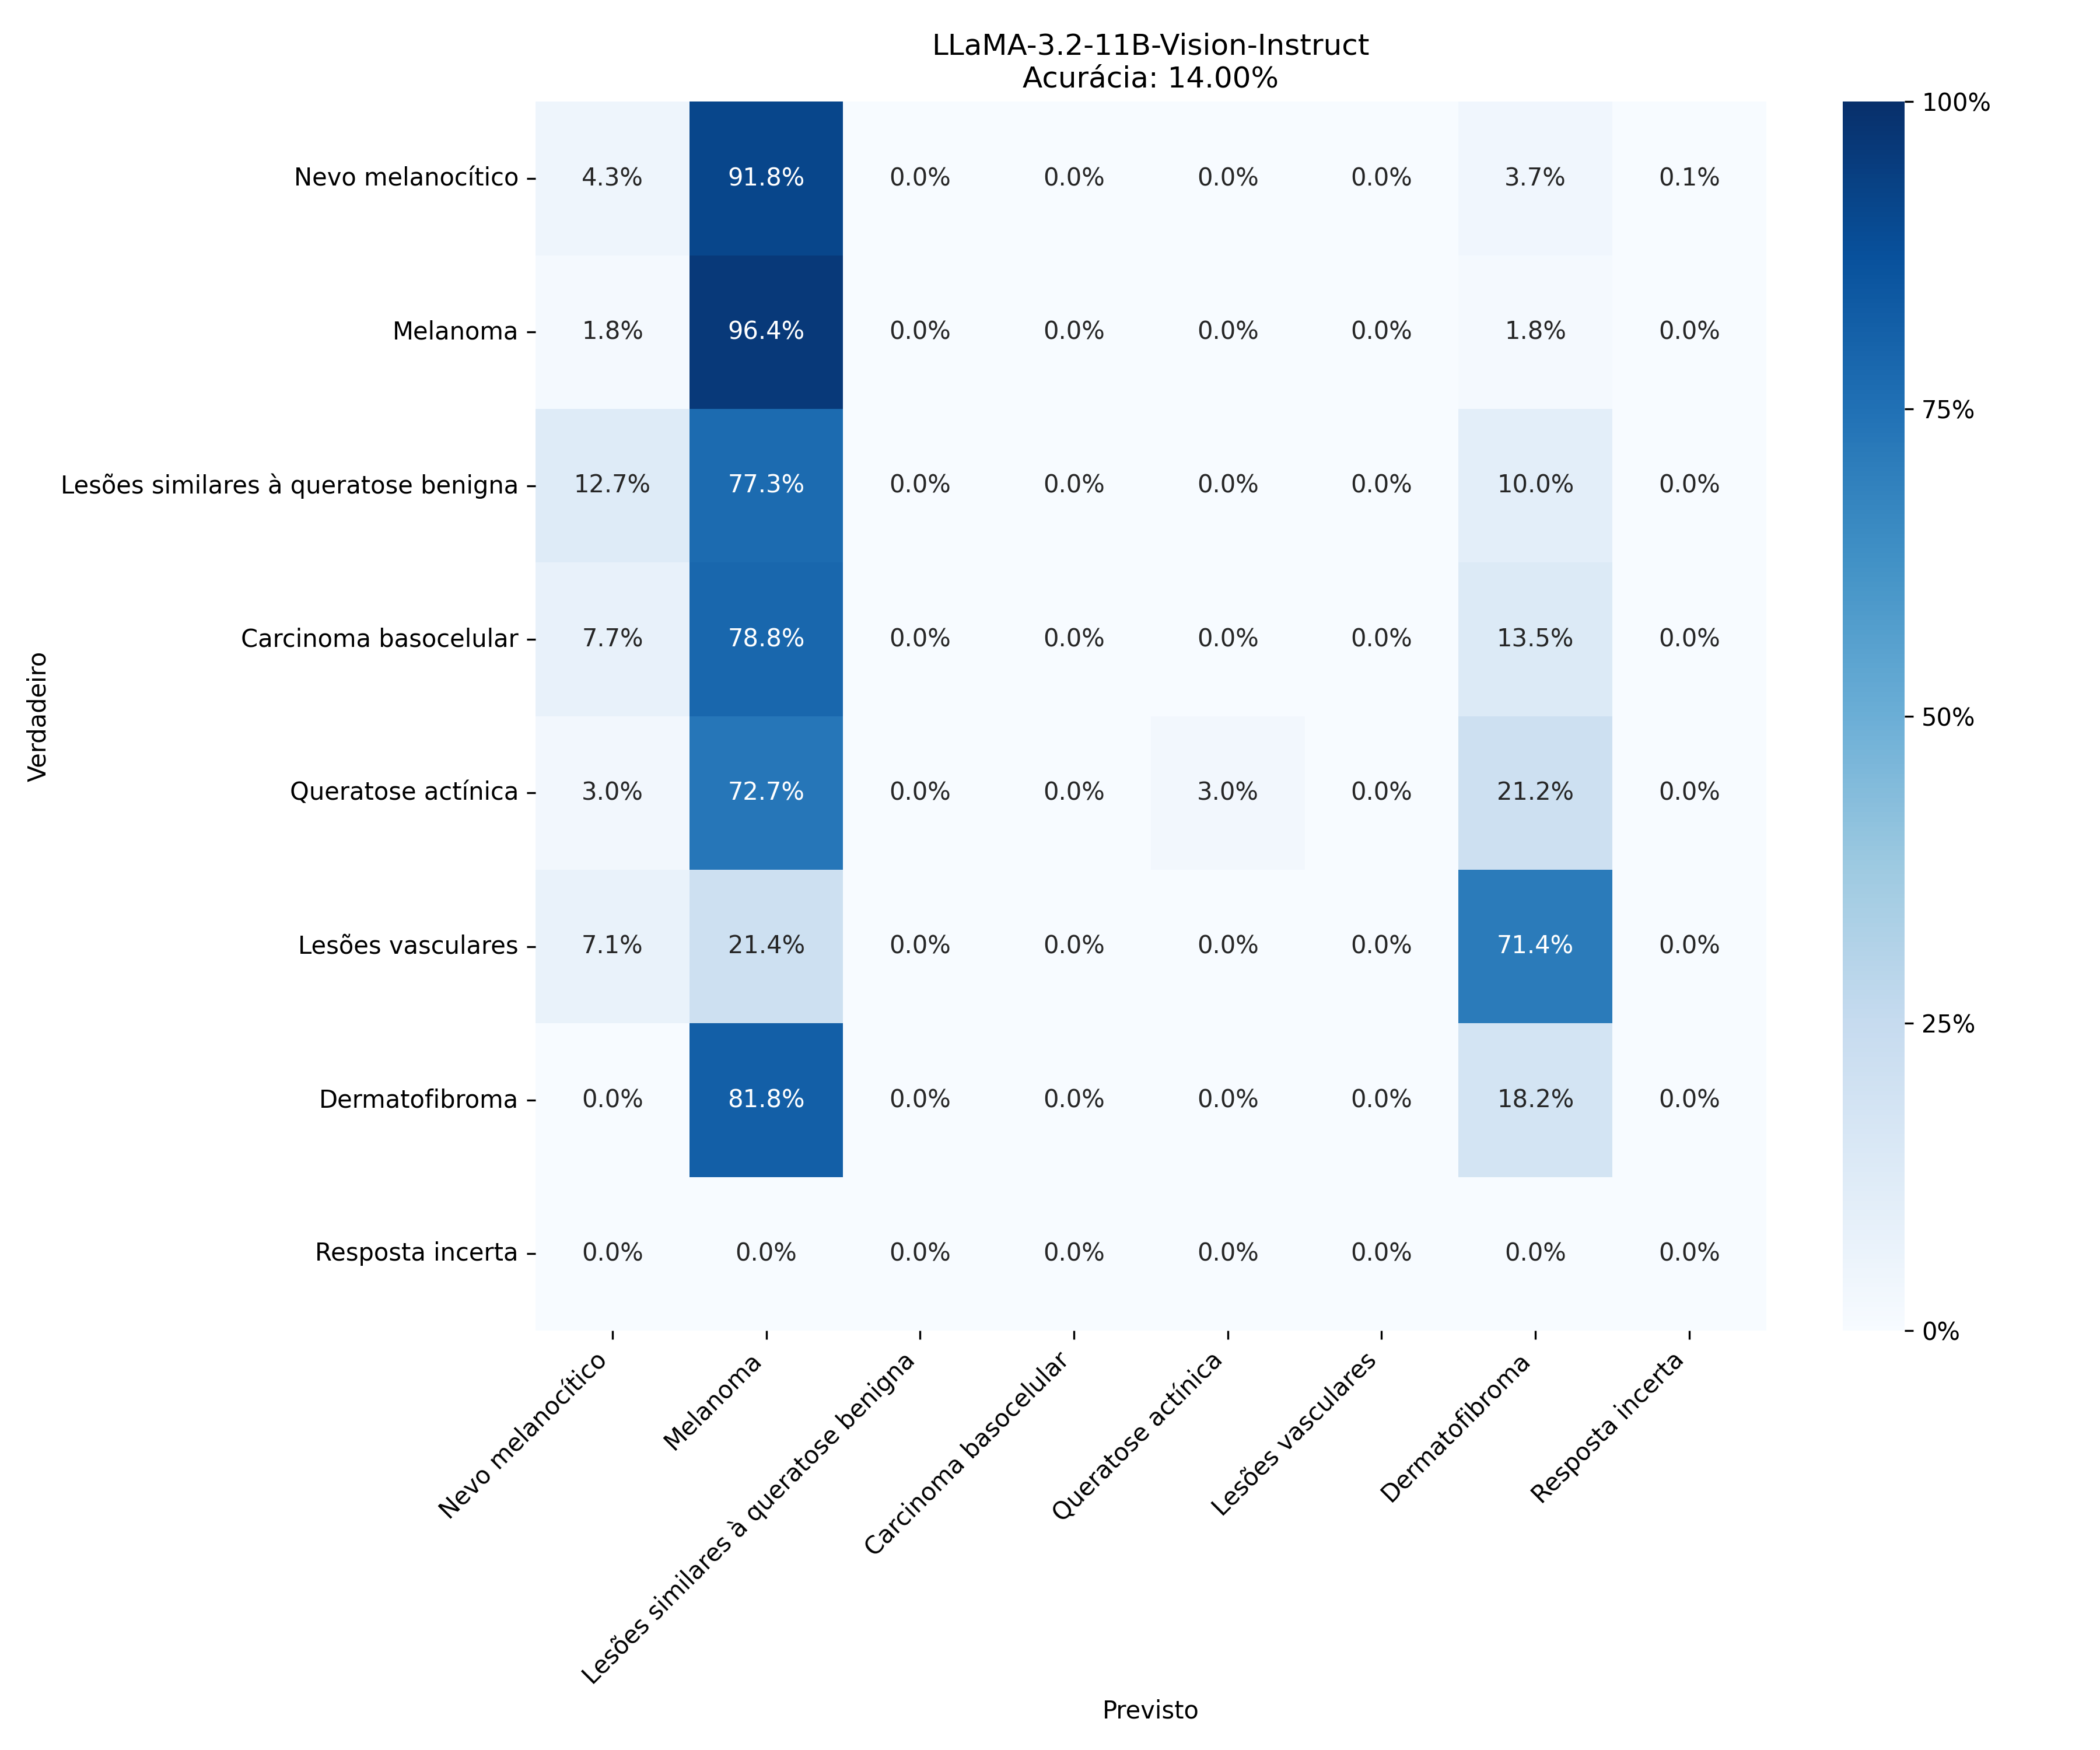
\includegraphics[width=1\columnwidth,keepaspectratio]{images/confusion_matrix_llama_3.2_11b_vision_instruct.png}
    \label{fig:confusion_matrix_llama}
    \fonte{Autoria própria.}
\end{figure}

\subsection{Análise dos modelos após o \textit{fine-tuning}}

Para as perguntas livres, todos os modelos treinados responderam no formato especificado no treinamento. O primeiro diálogo abaixo apresenta uma classificação correta e
o segundo apresenta uma incorreta, ambas as respostas foram dadas pelo modelo treinado com \ac{QLoRA} com 450 amostras:

\begin{dialogue}
    \speak{Usuário} \textit{Classify the skin lesion in the image. \textbf{<imagem de um nevo melanocítico>}} \\
    \speak{Modelo} \textit{The skin lesion in the image is melanocytic Nevi.}
\end{dialogue}

\begin{dialogue}
    \speak{Usuário} \textit{Classify the skin lesion in the image. \textbf{<imagem de um nevo melanoma>}} \\
    \speak{Modelo} \textit{The skin lesion in the image is benign keratosis-like lesions.}
\end{dialogue}

Os modelos trainados com \ac{QLoRA} com 450, 5000 e 9500 amostras, e com \ac{LoRA} com 5000 amostras apresentaram um problema em que as respostas não obedecem ao formato
especificado na pergunta objetiva, respondendo com o texto completo.

A acurácia nas respostas às perguntas objetivas aumentou consideravelmente com o \textit{fine-tuning} com \ac{QLoRA}, chegando a atingir 65,5\%. Porém, o modelo gerado
com esse treinamento tende a classificar a maioria das lesões como nevo melanocítico, o que indica que a acurácia maior pode ser simplesmente devido a uma quantidade
maior de nevos melanocíticos nos dados de teste. Para o modelo treinado com \ac{LoRA}, o desempenho foi menor, atingindo apenas 49,5\% de acurácia.

Em geral, como pode ser visto na \autoref{fig:confusion_matrix_qlora_450} e \autoref{fig:confusion_matrix_lora_450}, as duas versões ficaram insatisfatórias, o que se
deve a um treinamento com um conjunto pequeno de dados e hiperparâmetros não ideais.

\begin{figure}[ht]
    \centering
    \caption{\small Matriz de confusão para o \ac{LLaMA} treinado com \ac{QLoRA} e 450 amostras.}
    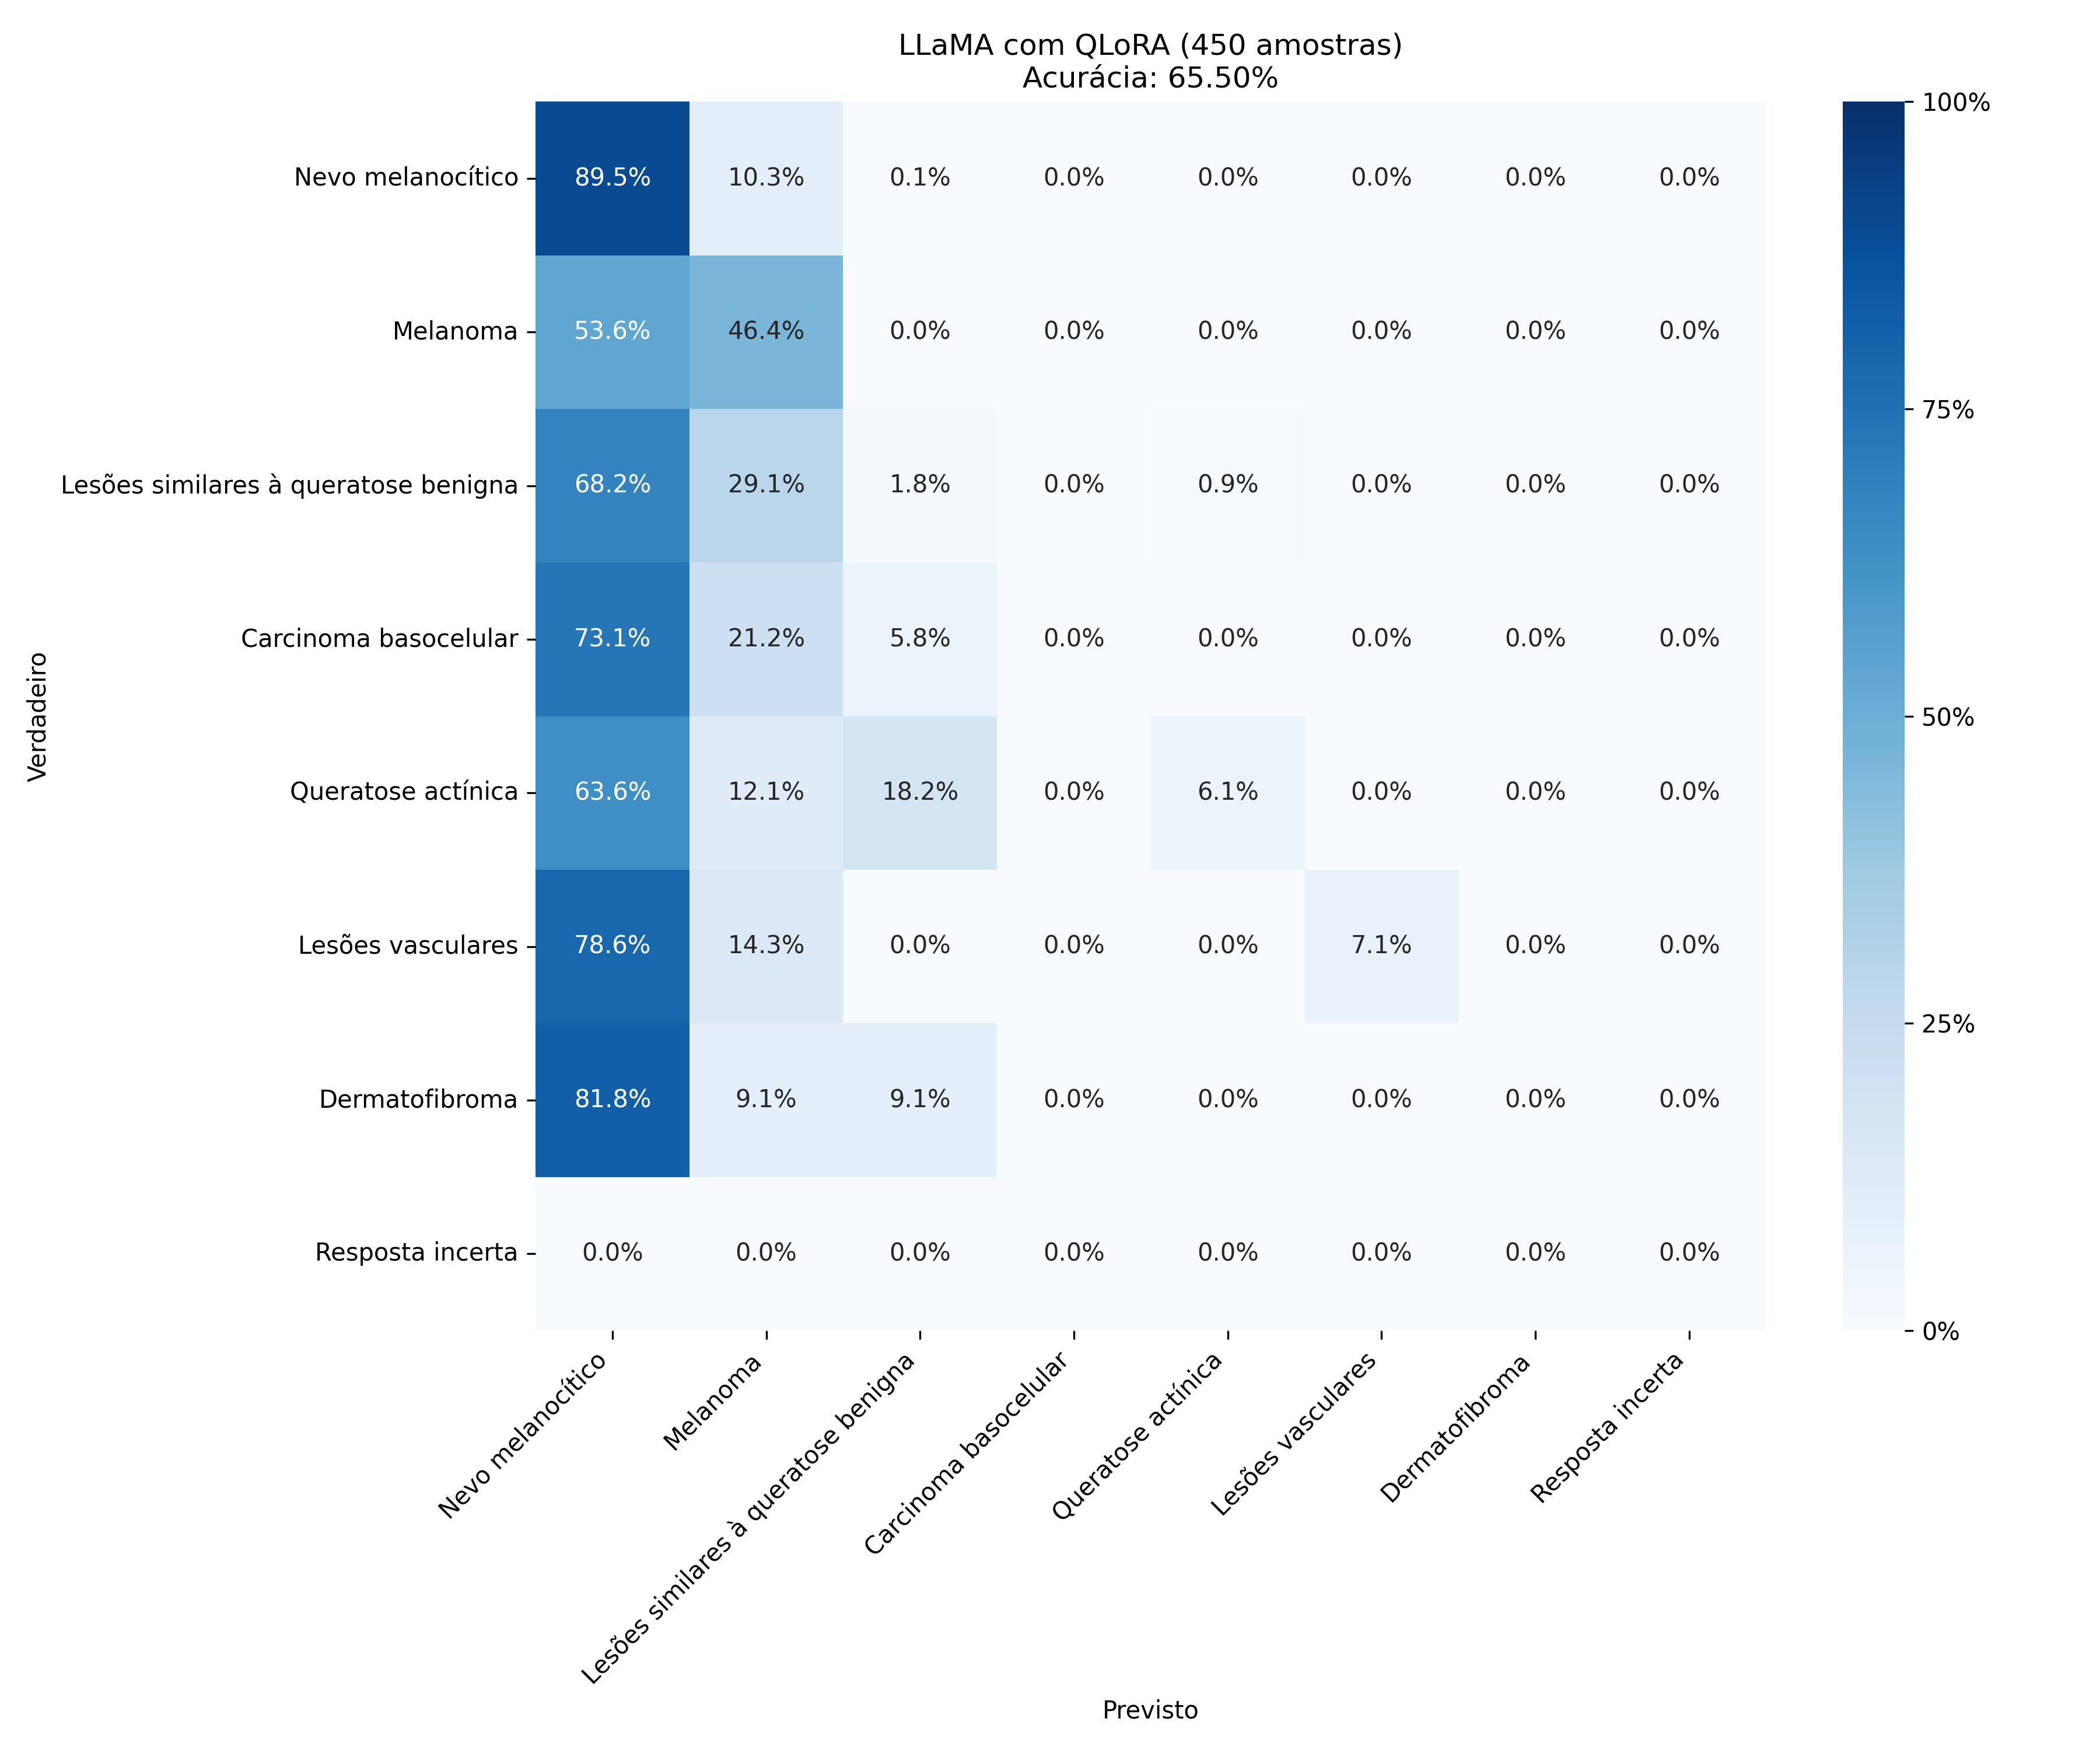
\includegraphics[width=1\columnwidth,keepaspectratio]{images/confusion_matrix_qlora_450.png}
    \label{fig:confusion_matrix_qlora_450}
    \fonte{Autoria própria.}
\end{figure}

\clearpage

\begin{figure}[ht]
    \centering
    \caption{\small Matriz de confusão para o \ac{LLaMA} treinado com \ac{LoRA} e 450 amostras.}
    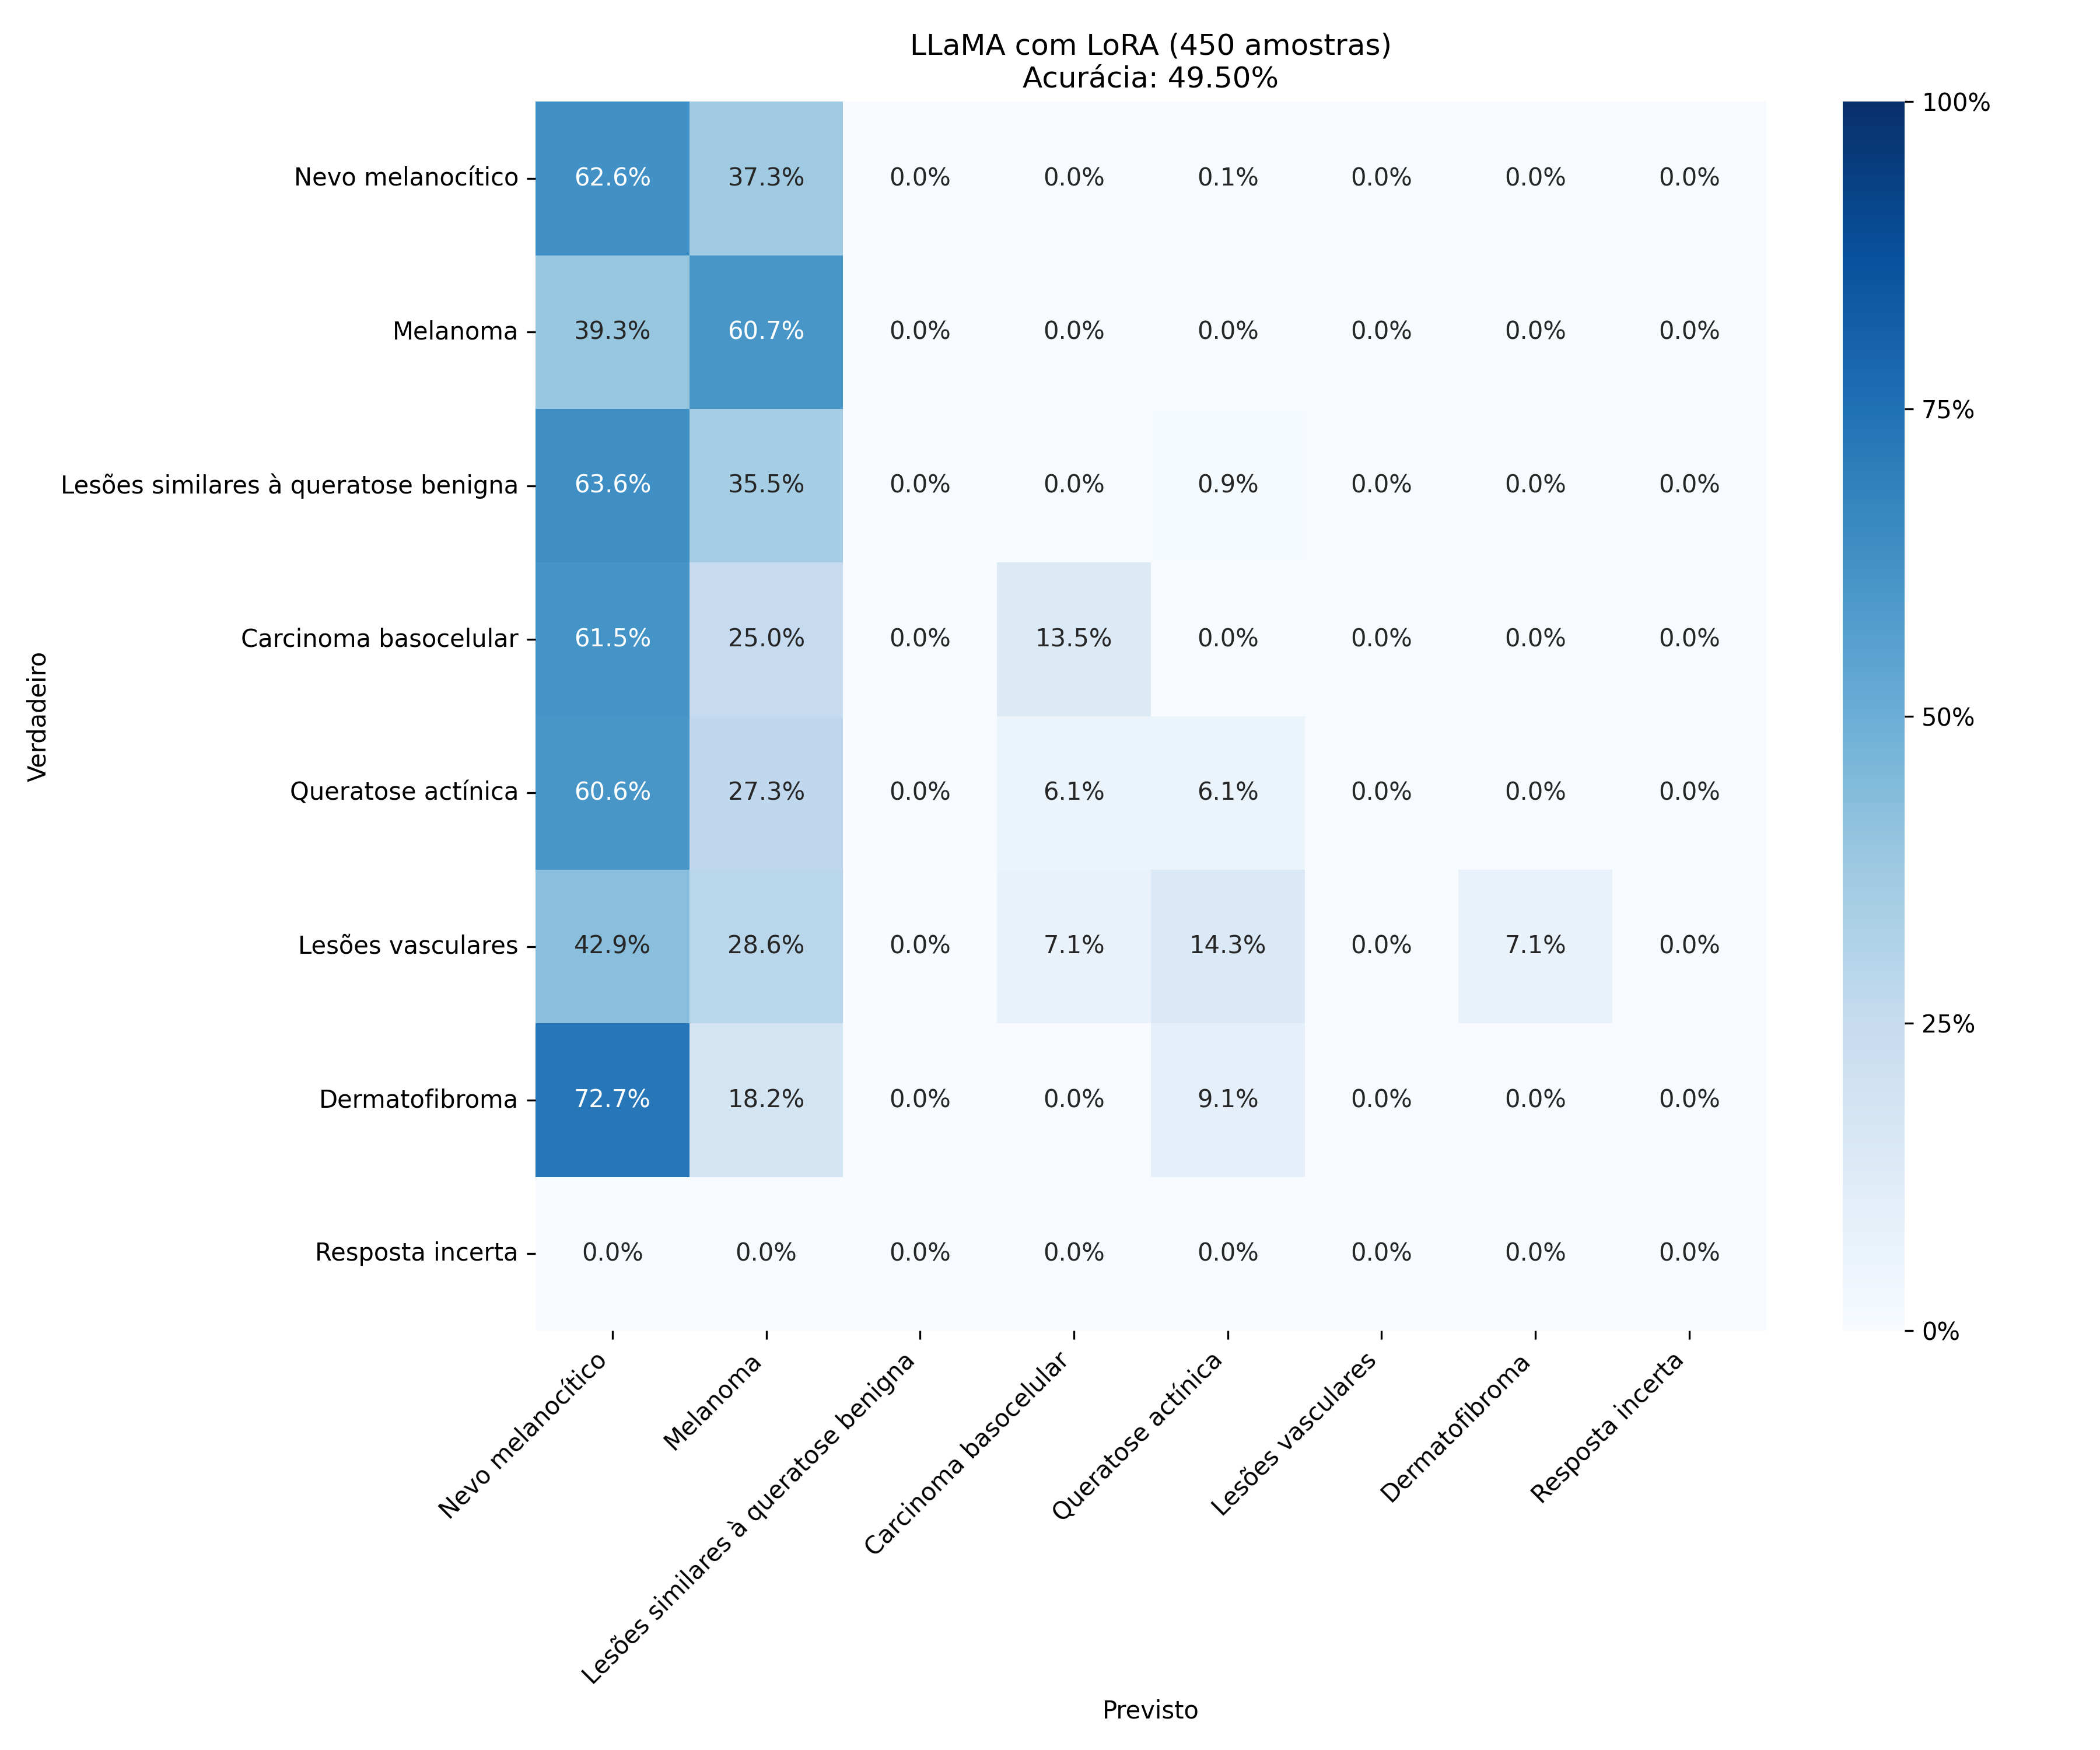
\includegraphics[width=1\columnwidth,keepaspectratio]{images/confusion_matrix_lora_450.png}
    \label{fig:confusion_matrix_lora_450}
    \fonte{Autoria própria.}
\end{figure}

A acurácia decaiu levemente no \textit{fine-tuning} com 900 amostas, conforme apresentado na \autoref{fig:confusion_matrix_qlora_900} e
\autoref{fig:confusion_matrix_lora_900}, ficando em 65.2\% para o \ac{LLaMA} treinado com \ac{QLoRA} e 42\% para o treinado com \ac{LoRA}. Porém, o modelo treinado com
\ac{QLoRA} apresenta um padrão melhor de classificação, reconhecendo melhor as lesões de nevos melanocíticos e de queratoses actínicas.

\clearpage

\begin{figure}[ht]
    \centering
    \caption{\small Matriz de confusão para o \ac{LLaMA} treinado com \ac{QLoRA} e 900 amostras.}
    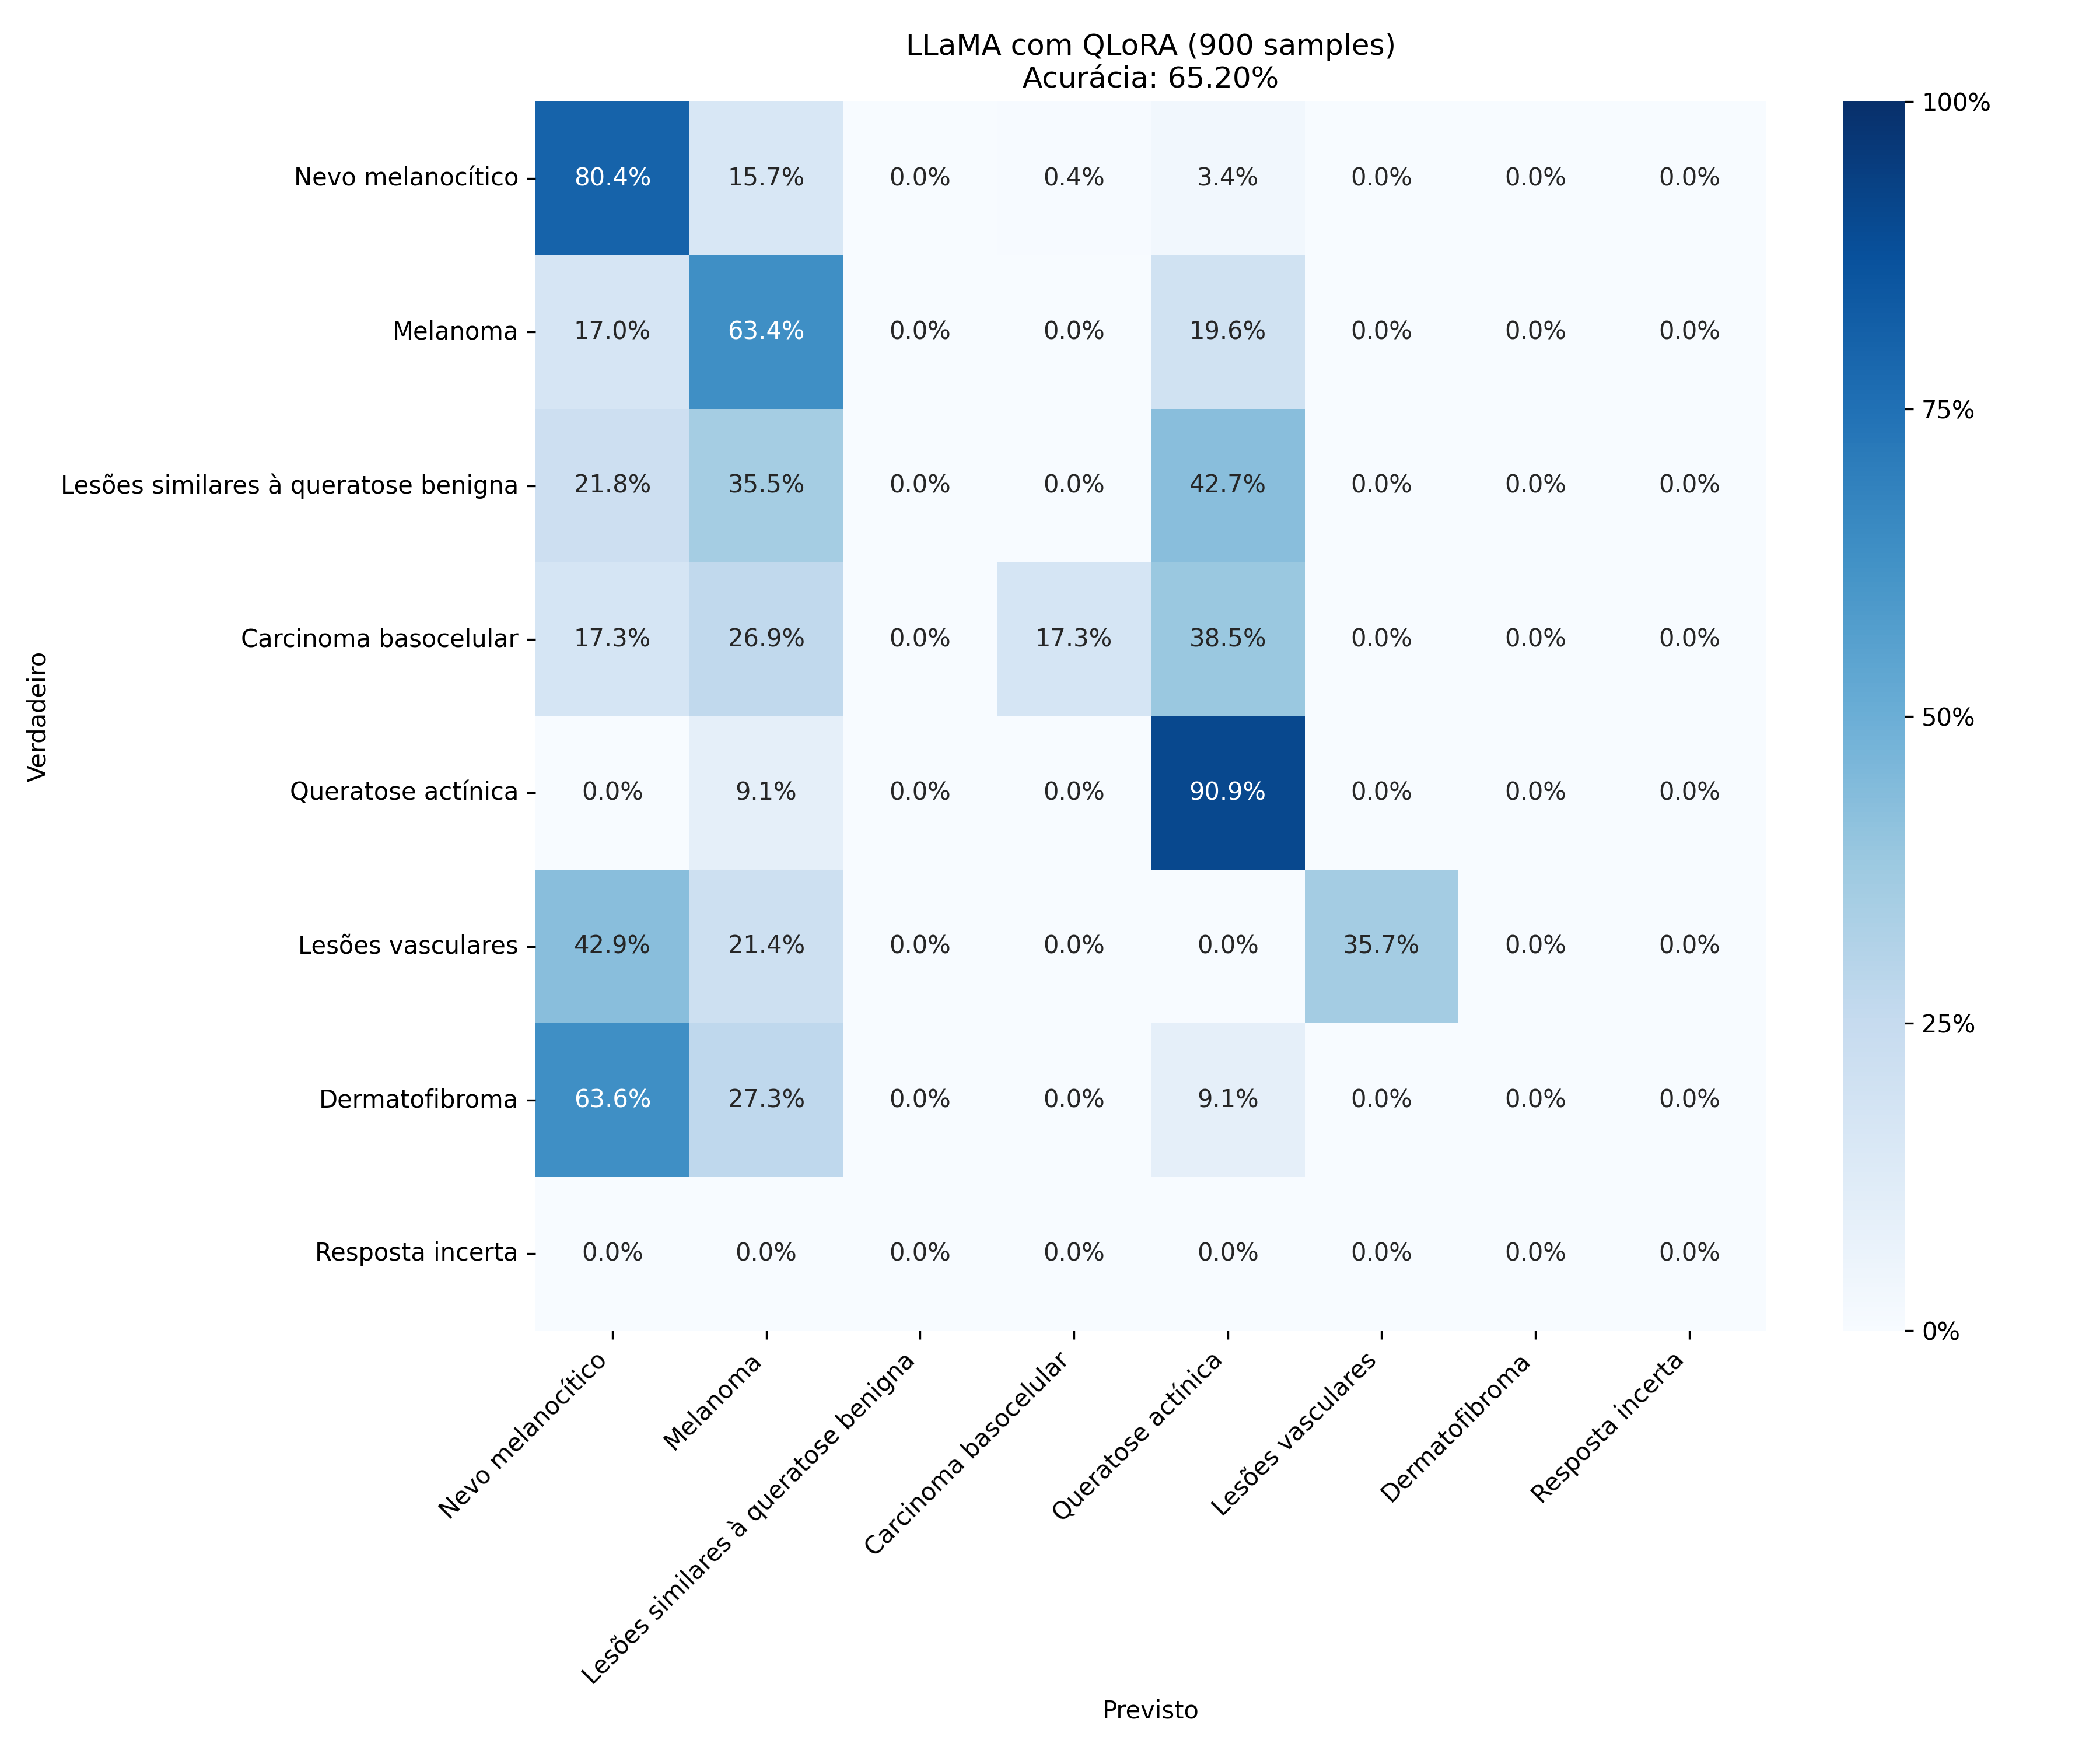
\includegraphics[width=1\columnwidth,keepaspectratio]{images/confusion_matrix_qlora_900.png}
    \label{fig:confusion_matrix_qlora_900}
    \fonte{Autoria própria.}
\end{figure}

\clearpage

\begin{figure}[ht]
    \centering
    \caption{\small Matriz de confusão para o \ac{LLaMA} treinado com \ac{LoRA} e 900 amostras.}
    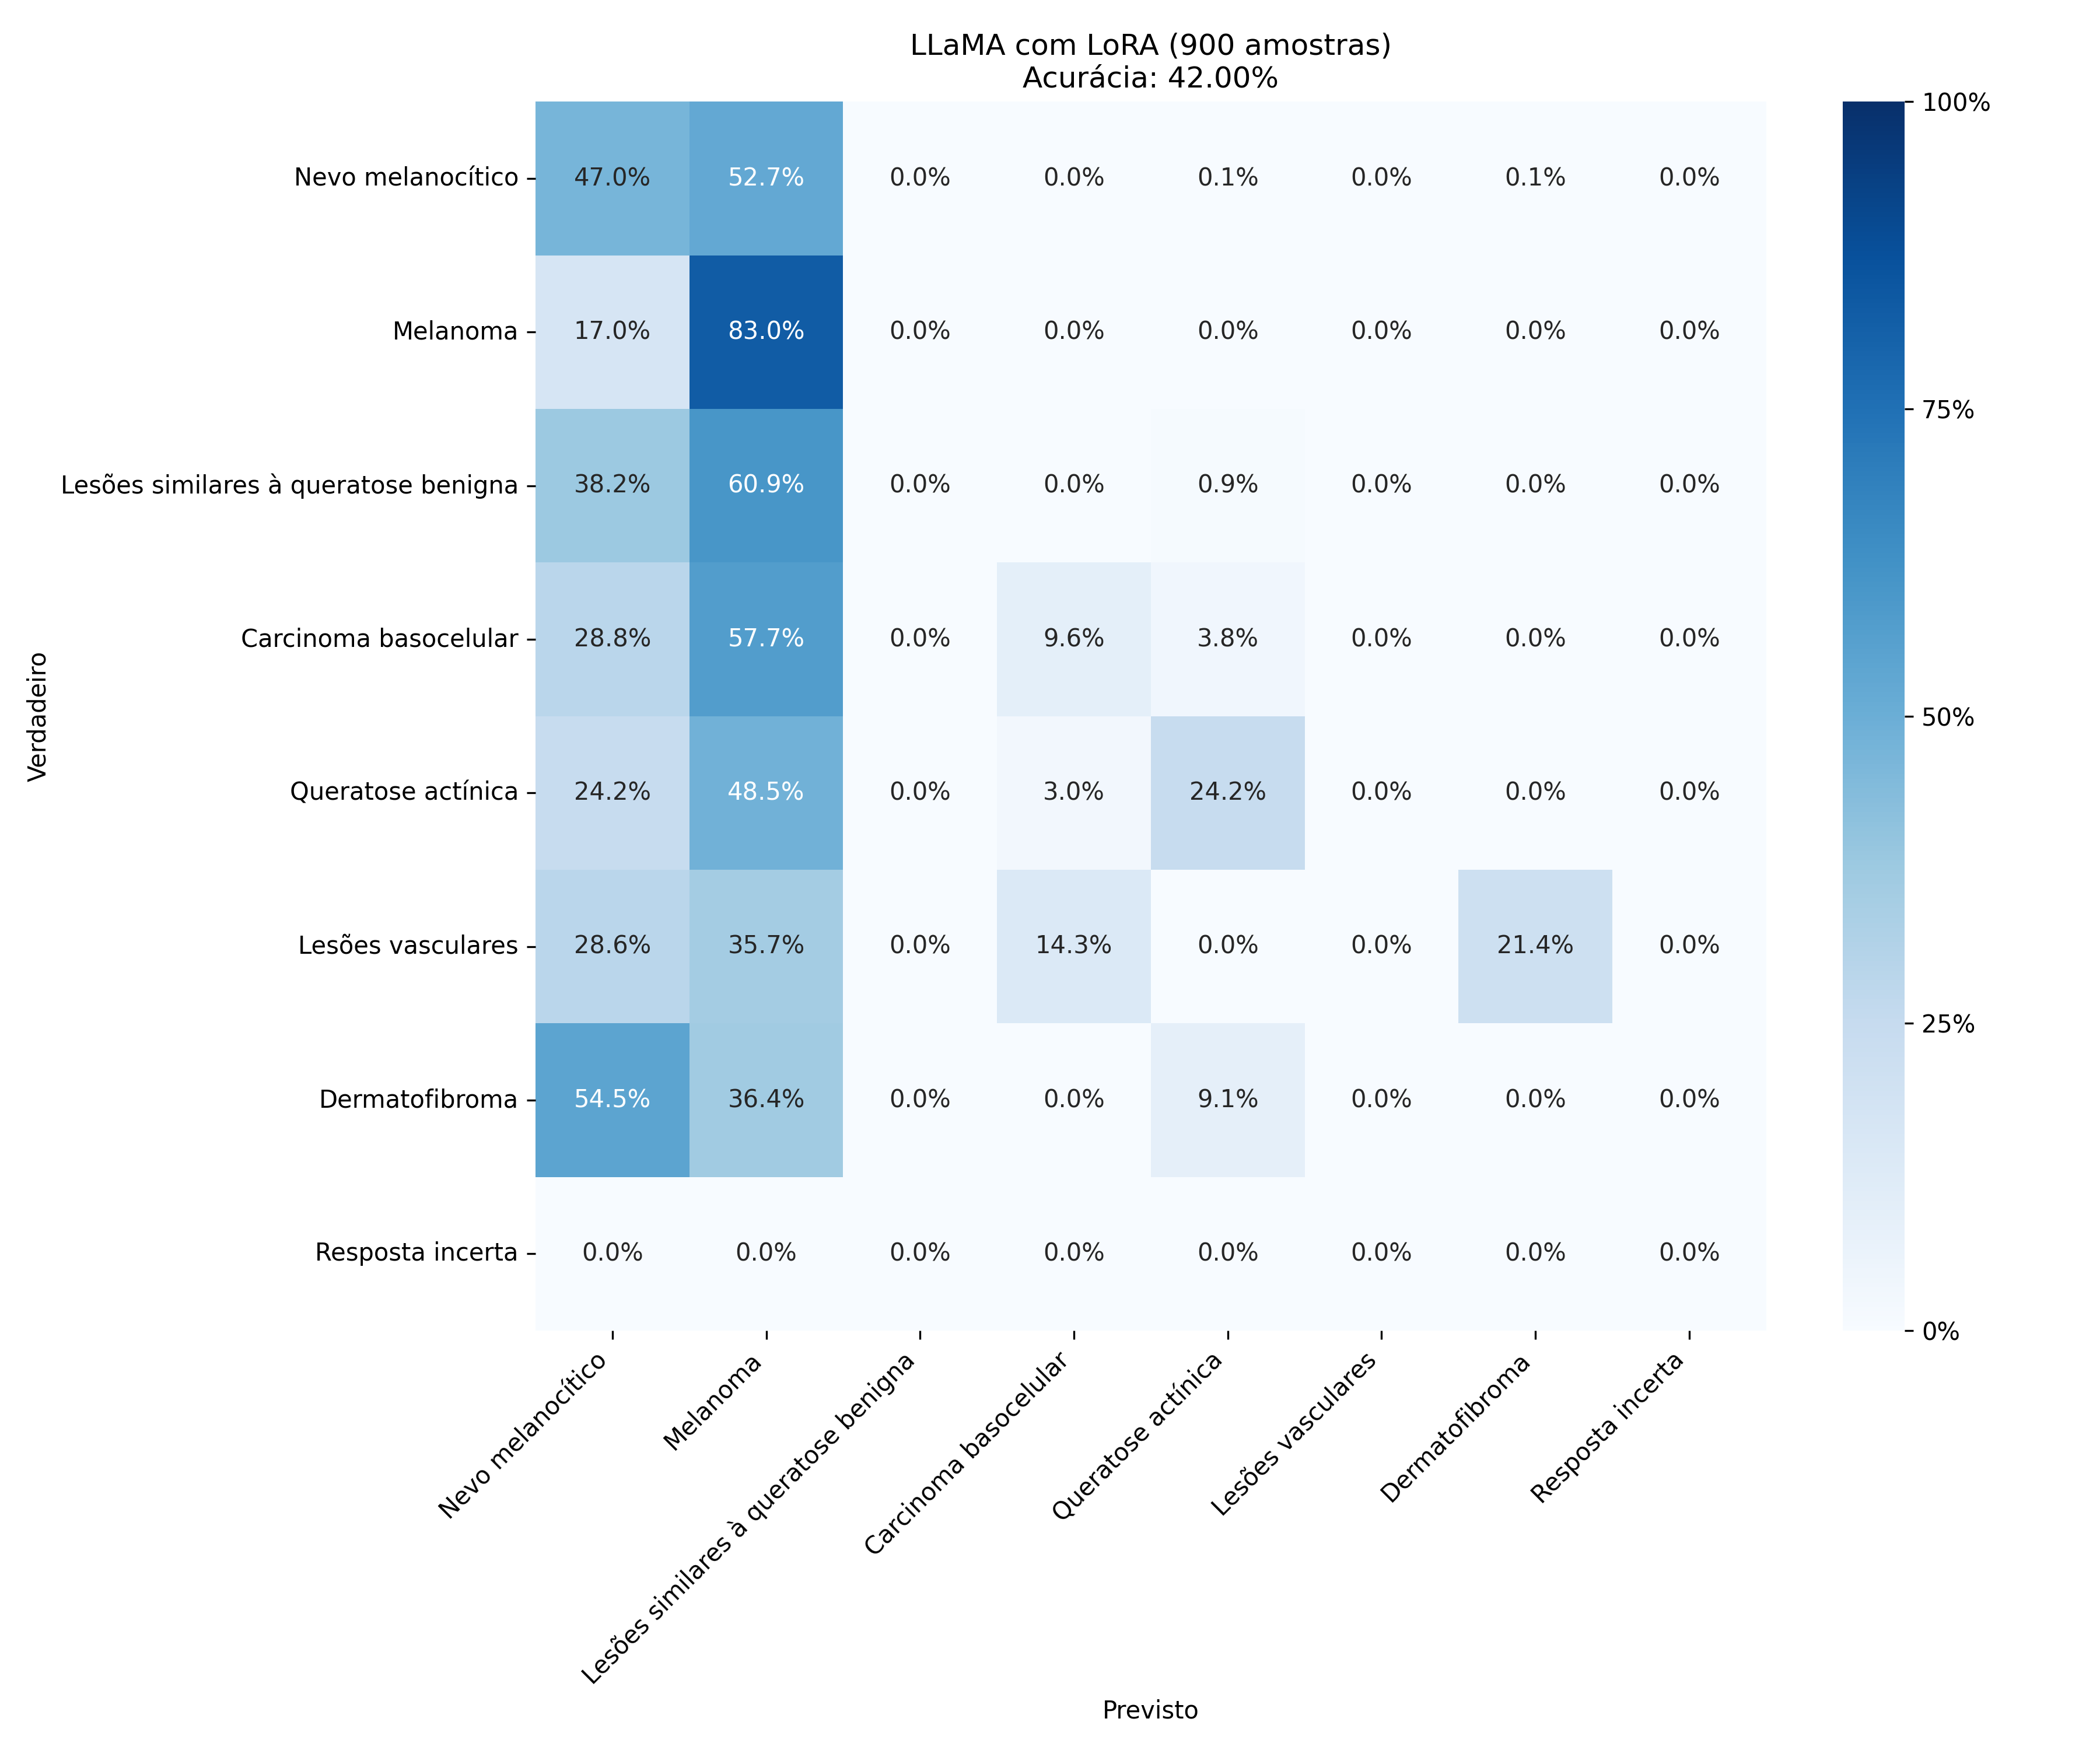
\includegraphics[width=1\columnwidth,keepaspectratio]{images/confusion_matrix_lora_900.png}
    \label{fig:confusion_matrix_lora_900}
    \fonte{Autoria própria.}
\end{figure}


O modelo treinado com \ac{QLoRA} e 1800 amostras teve um ganho de acurácia, atingindo 71,1\% e apresentando um padrão de reconhecimento melhor do que os modelos
anteriores. A matriz de confusão pode ser vista na \autoref{fig:confusion_matrix_qlora_1800}.

\clearpage

\begin{figure}[ht]
    \centering
    \caption{\small Matriz de confusão para o \ac{LLaMA} treinado com \ac{QLoRA} e 1800 amostras.}
    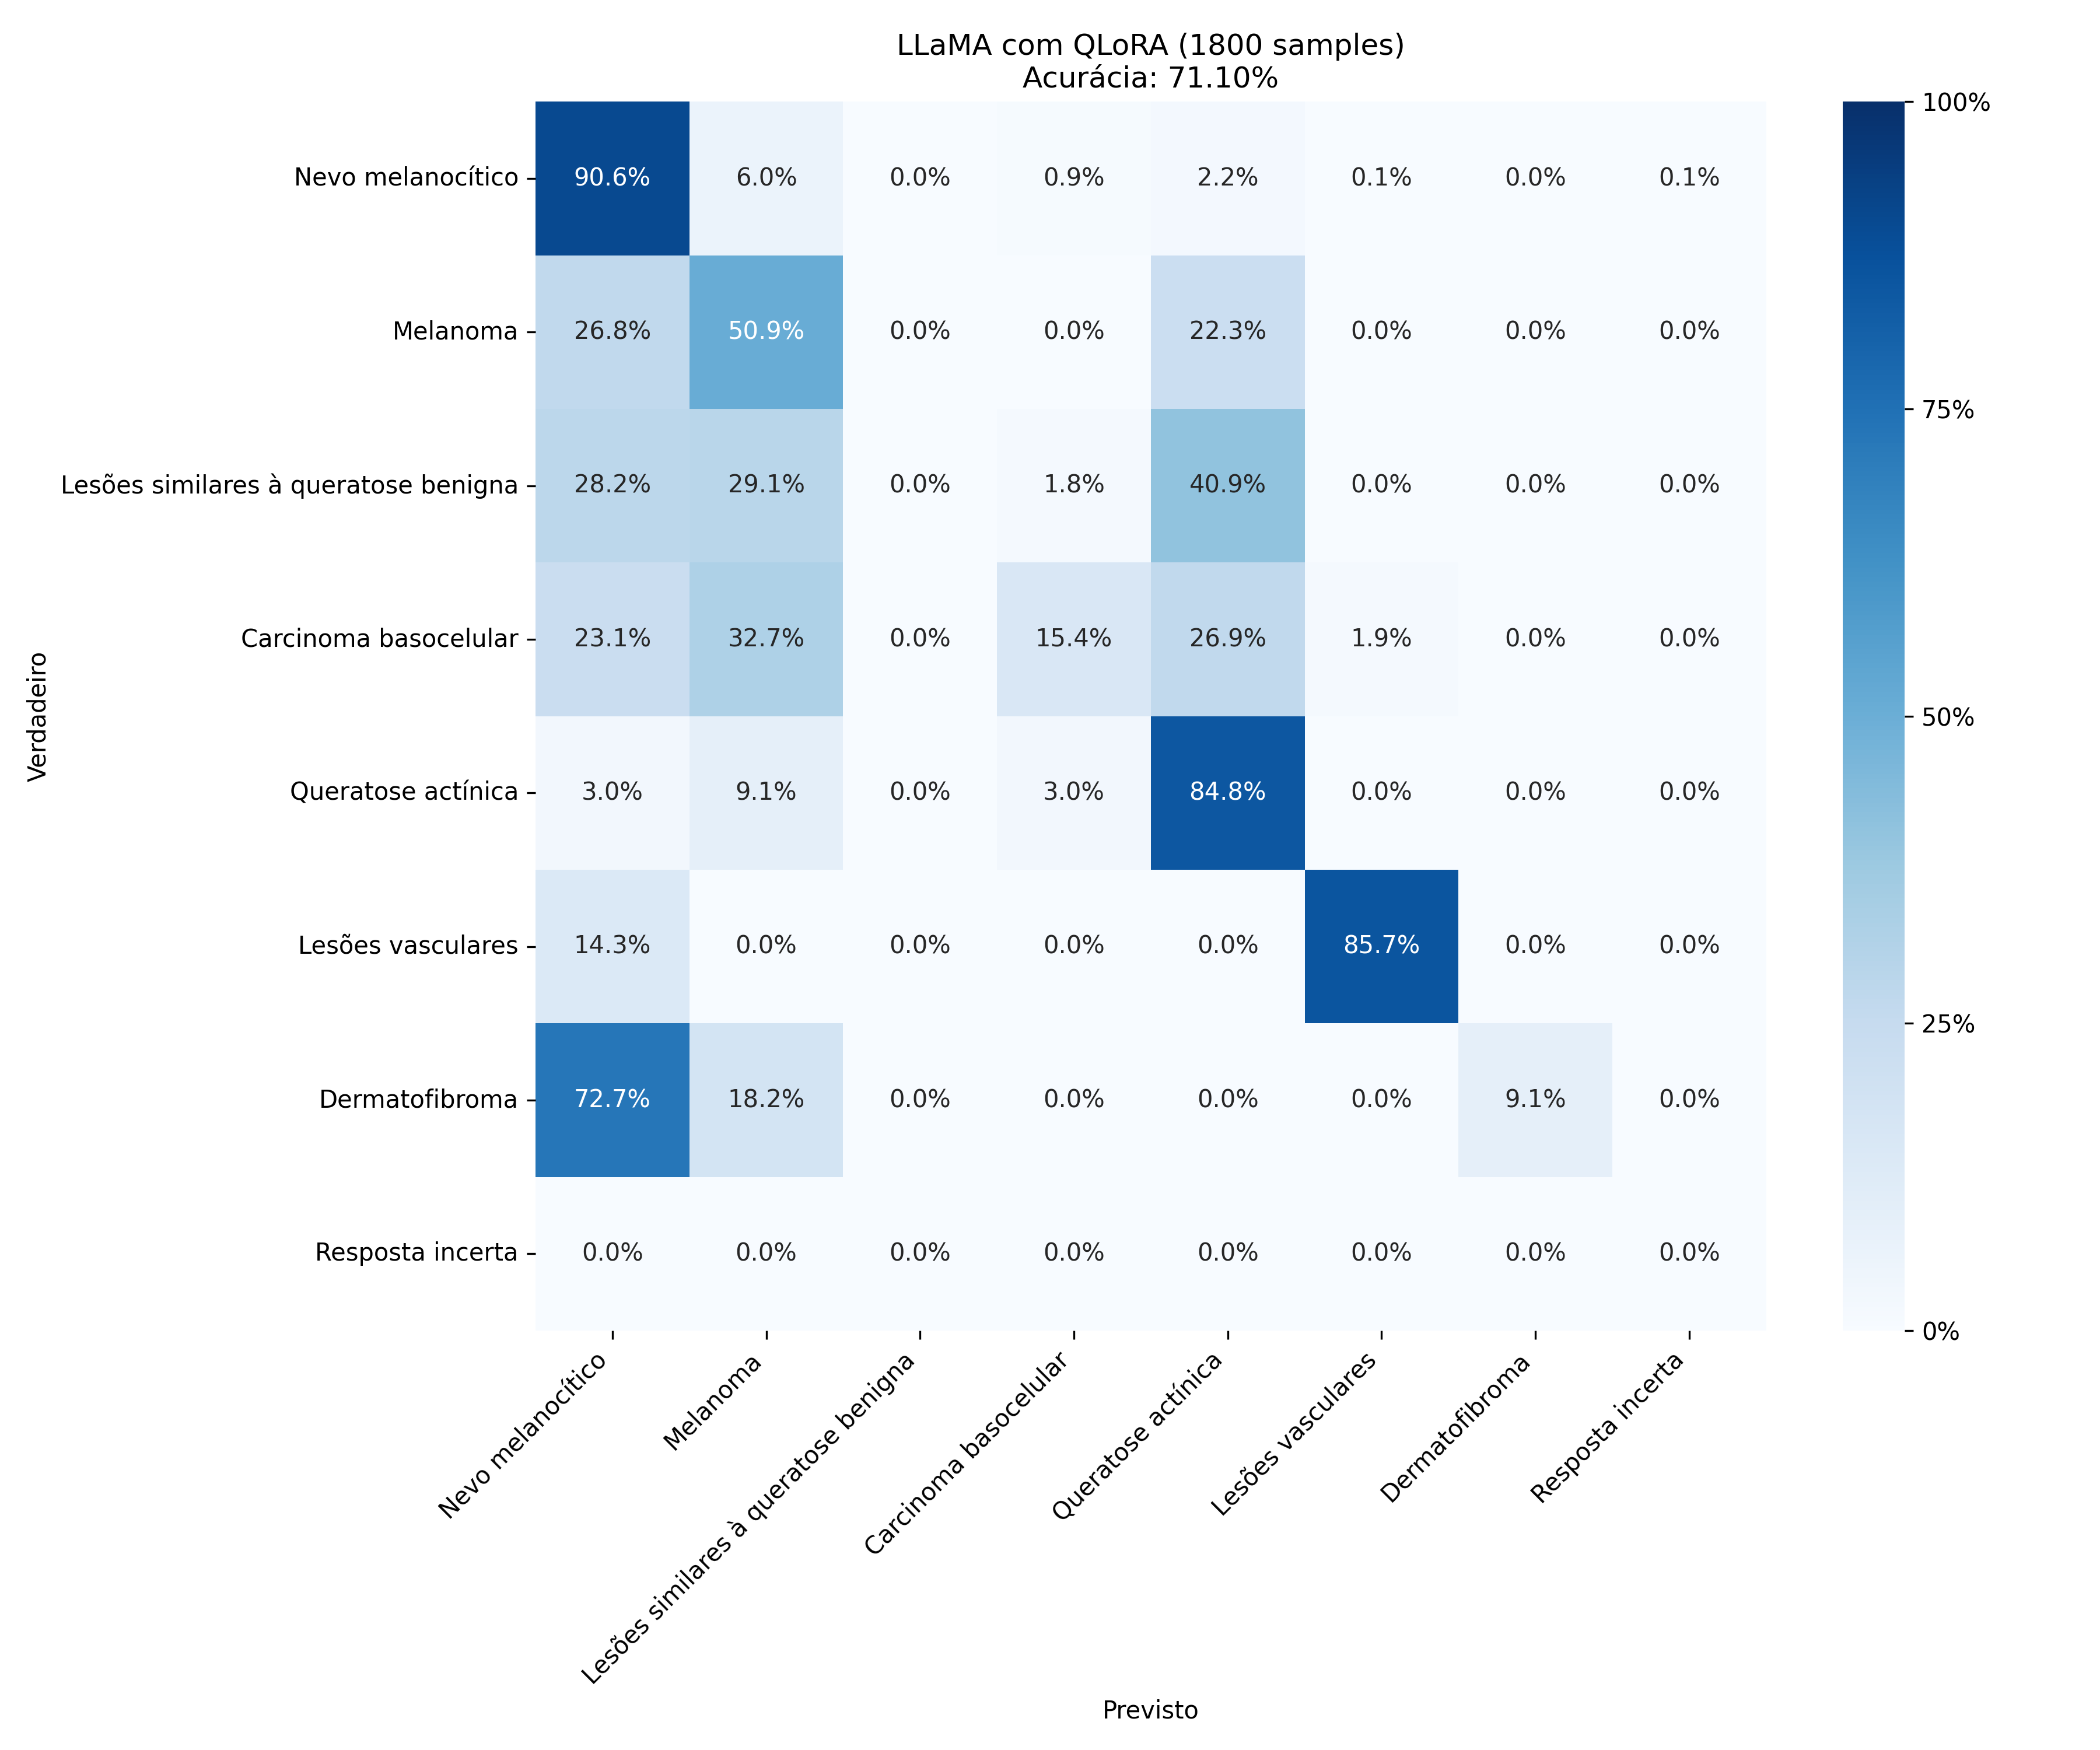
\includegraphics[width=1\columnwidth,keepaspectratio]{images/confusion_matrix_qlora_1800.png}
    \label{fig:confusion_matrix_qlora_1800}
    \fonte{Autoria própria.}
\end{figure}

Com 5000 amostras, ambos os modelos treinados com \ac{QLoRA} e \ac{LoRA} apresentaram resultados melhores, com 85,4\% e 86,2\% de acurácia, respectivamente. Deve-se
observar que as configurações de treinamento foram modificadas, sendo que os dois métodos utilizam hiperparâmetros similares. O \textit{fine-tuning} com \ac{LoRA} se
mostrou levemente melhor dessa vez, demonstrando que o baixo desempenho do \ac{LoRA} nos outros treinamentos foi por conta de uma escolha não ideal de hiperparâmetros.
A \autoref{fig:confusion_matrix_qlora_5000} e a \autoref{fig:confusion_matrix_lora_5000} apresentam esses resultados.

\clearpage

\begin{figure}[ht]
    \centering
    \caption{\small Matriz de confusão do \ac{LLaMA} treinado com \ac{QLoRA} e 5000 amostras.}
    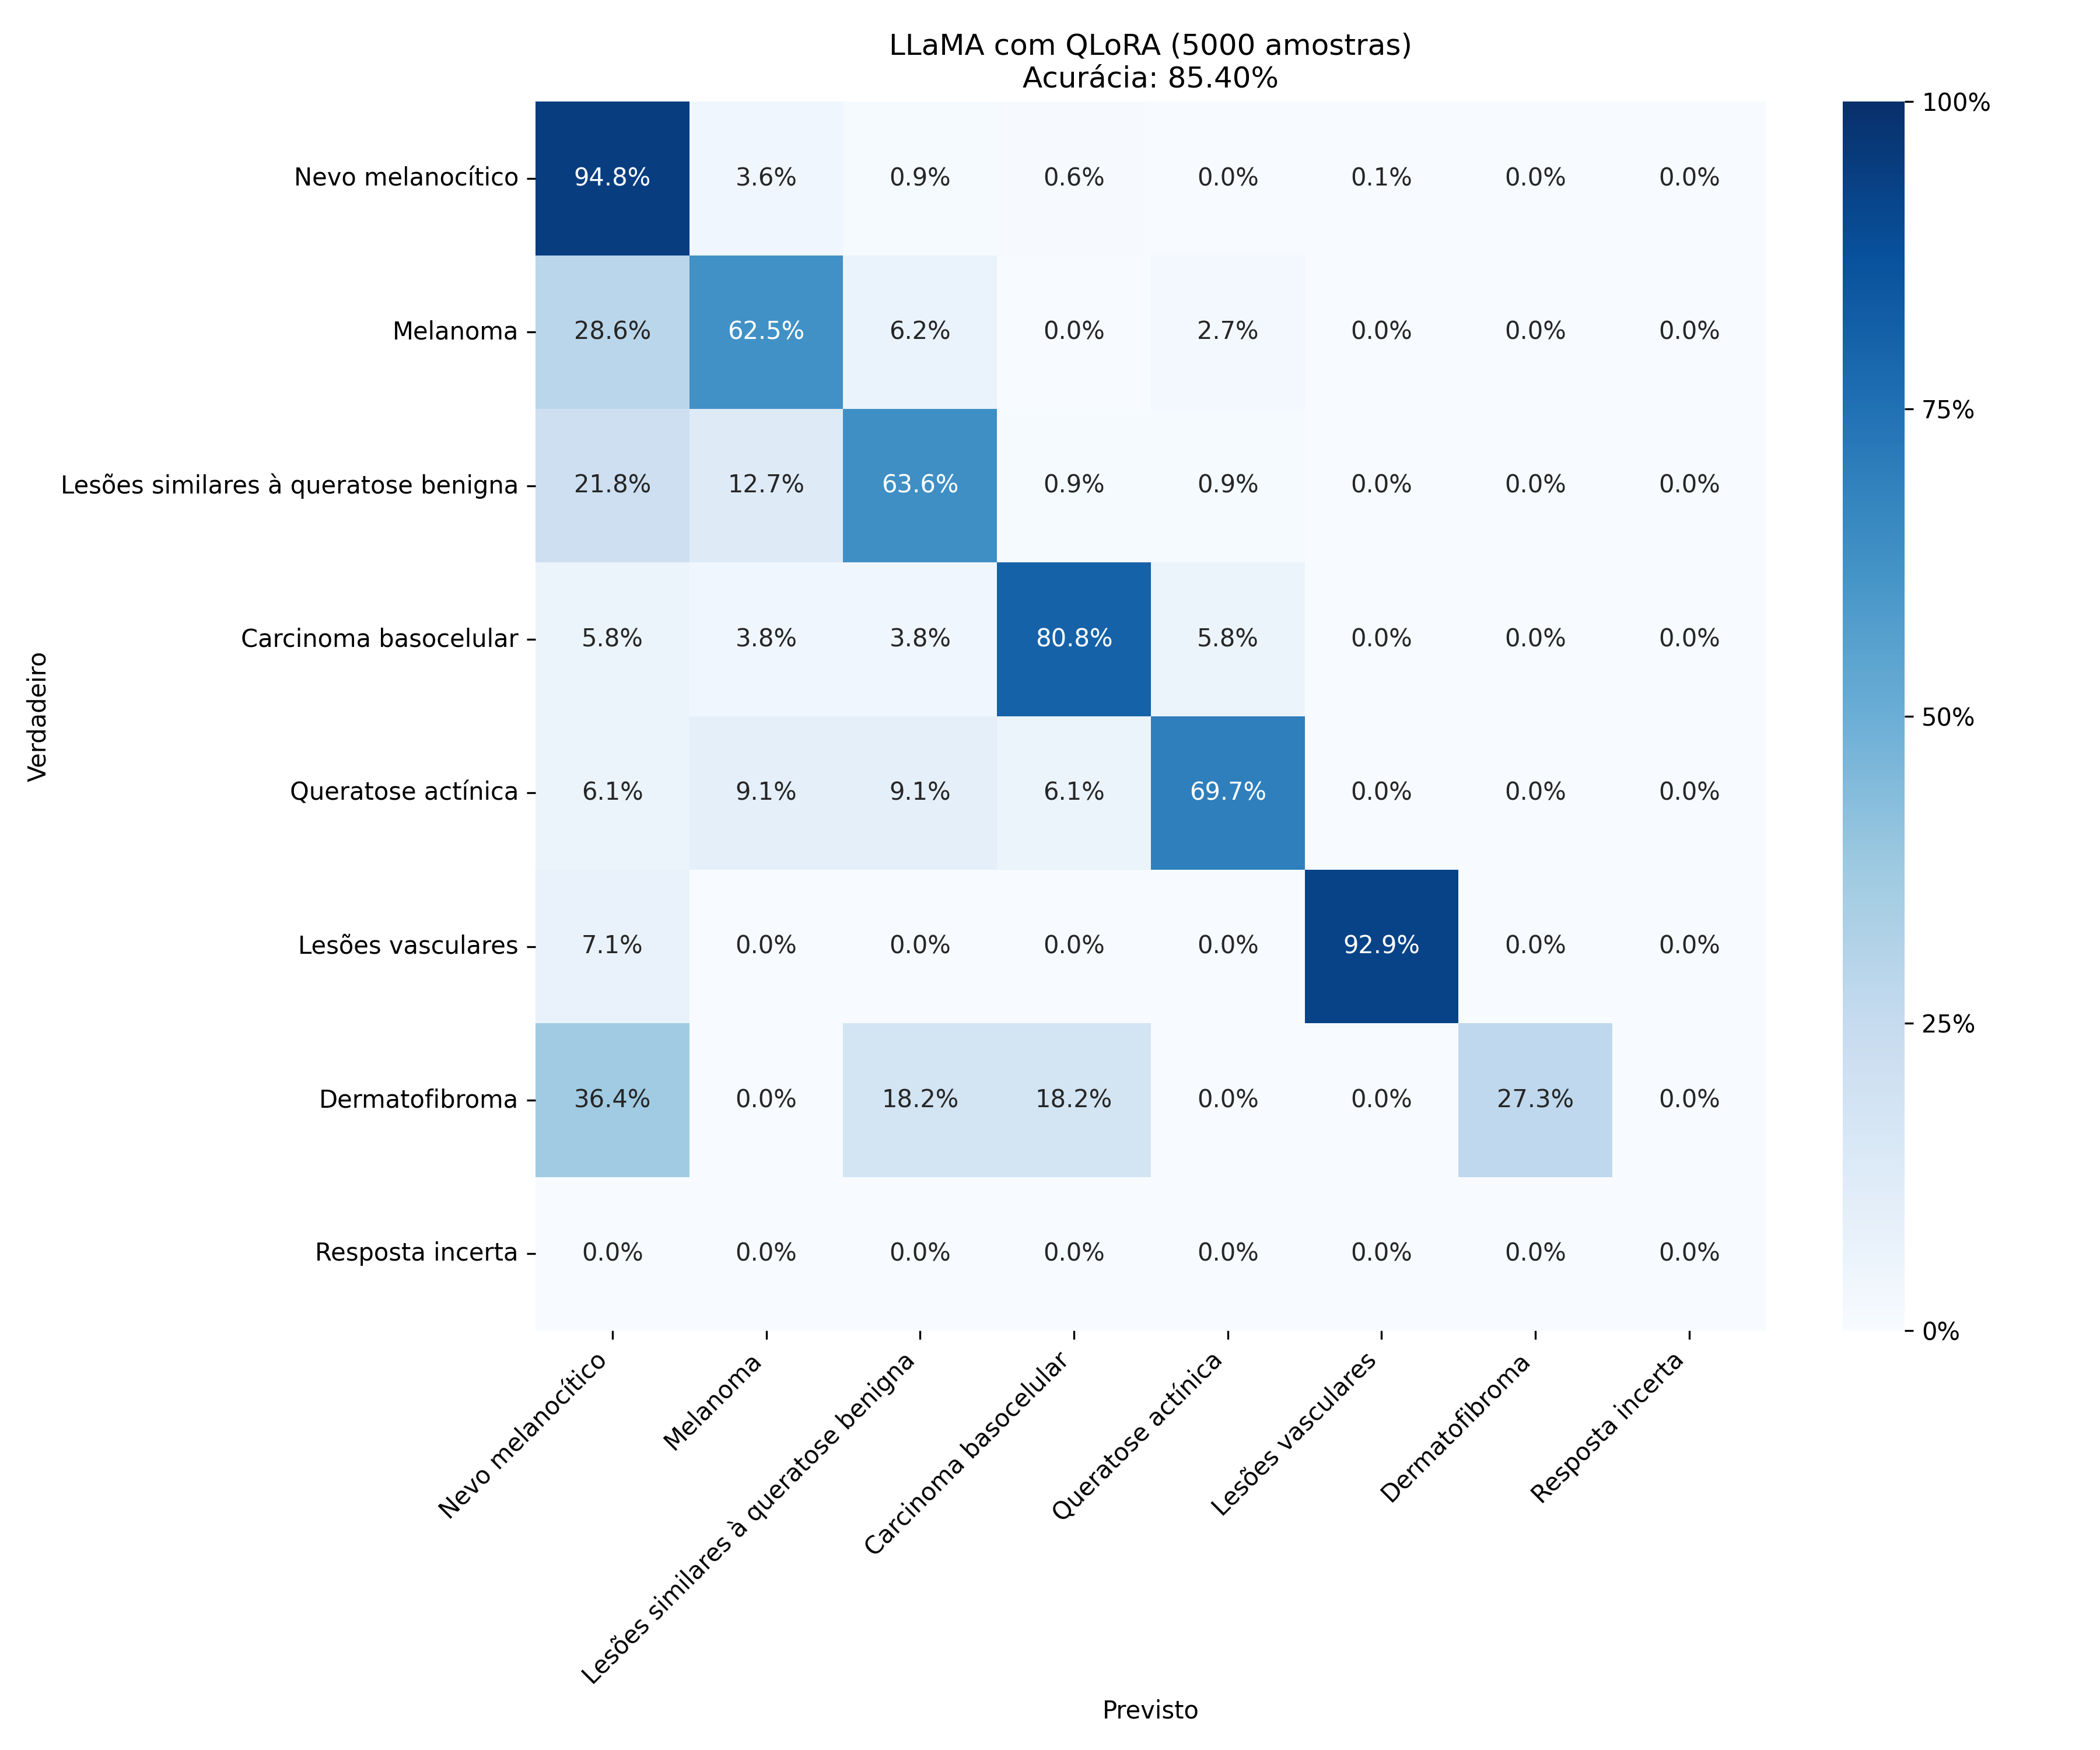
\includegraphics[width=1\columnwidth,keepaspectratio]{images/confusion_matrix_qlora_5000.png}
    \label{fig:confusion_matrix_qlora_5000}
    \fonte{Autoria própria.}
\end{figure}

\clearpage

\begin{figure}[ht]
    \centering
    \caption{\small Matriz de confusão para o \ac{LLaMA} treinado com \ac{LoRA} e 5000 amostras.}
    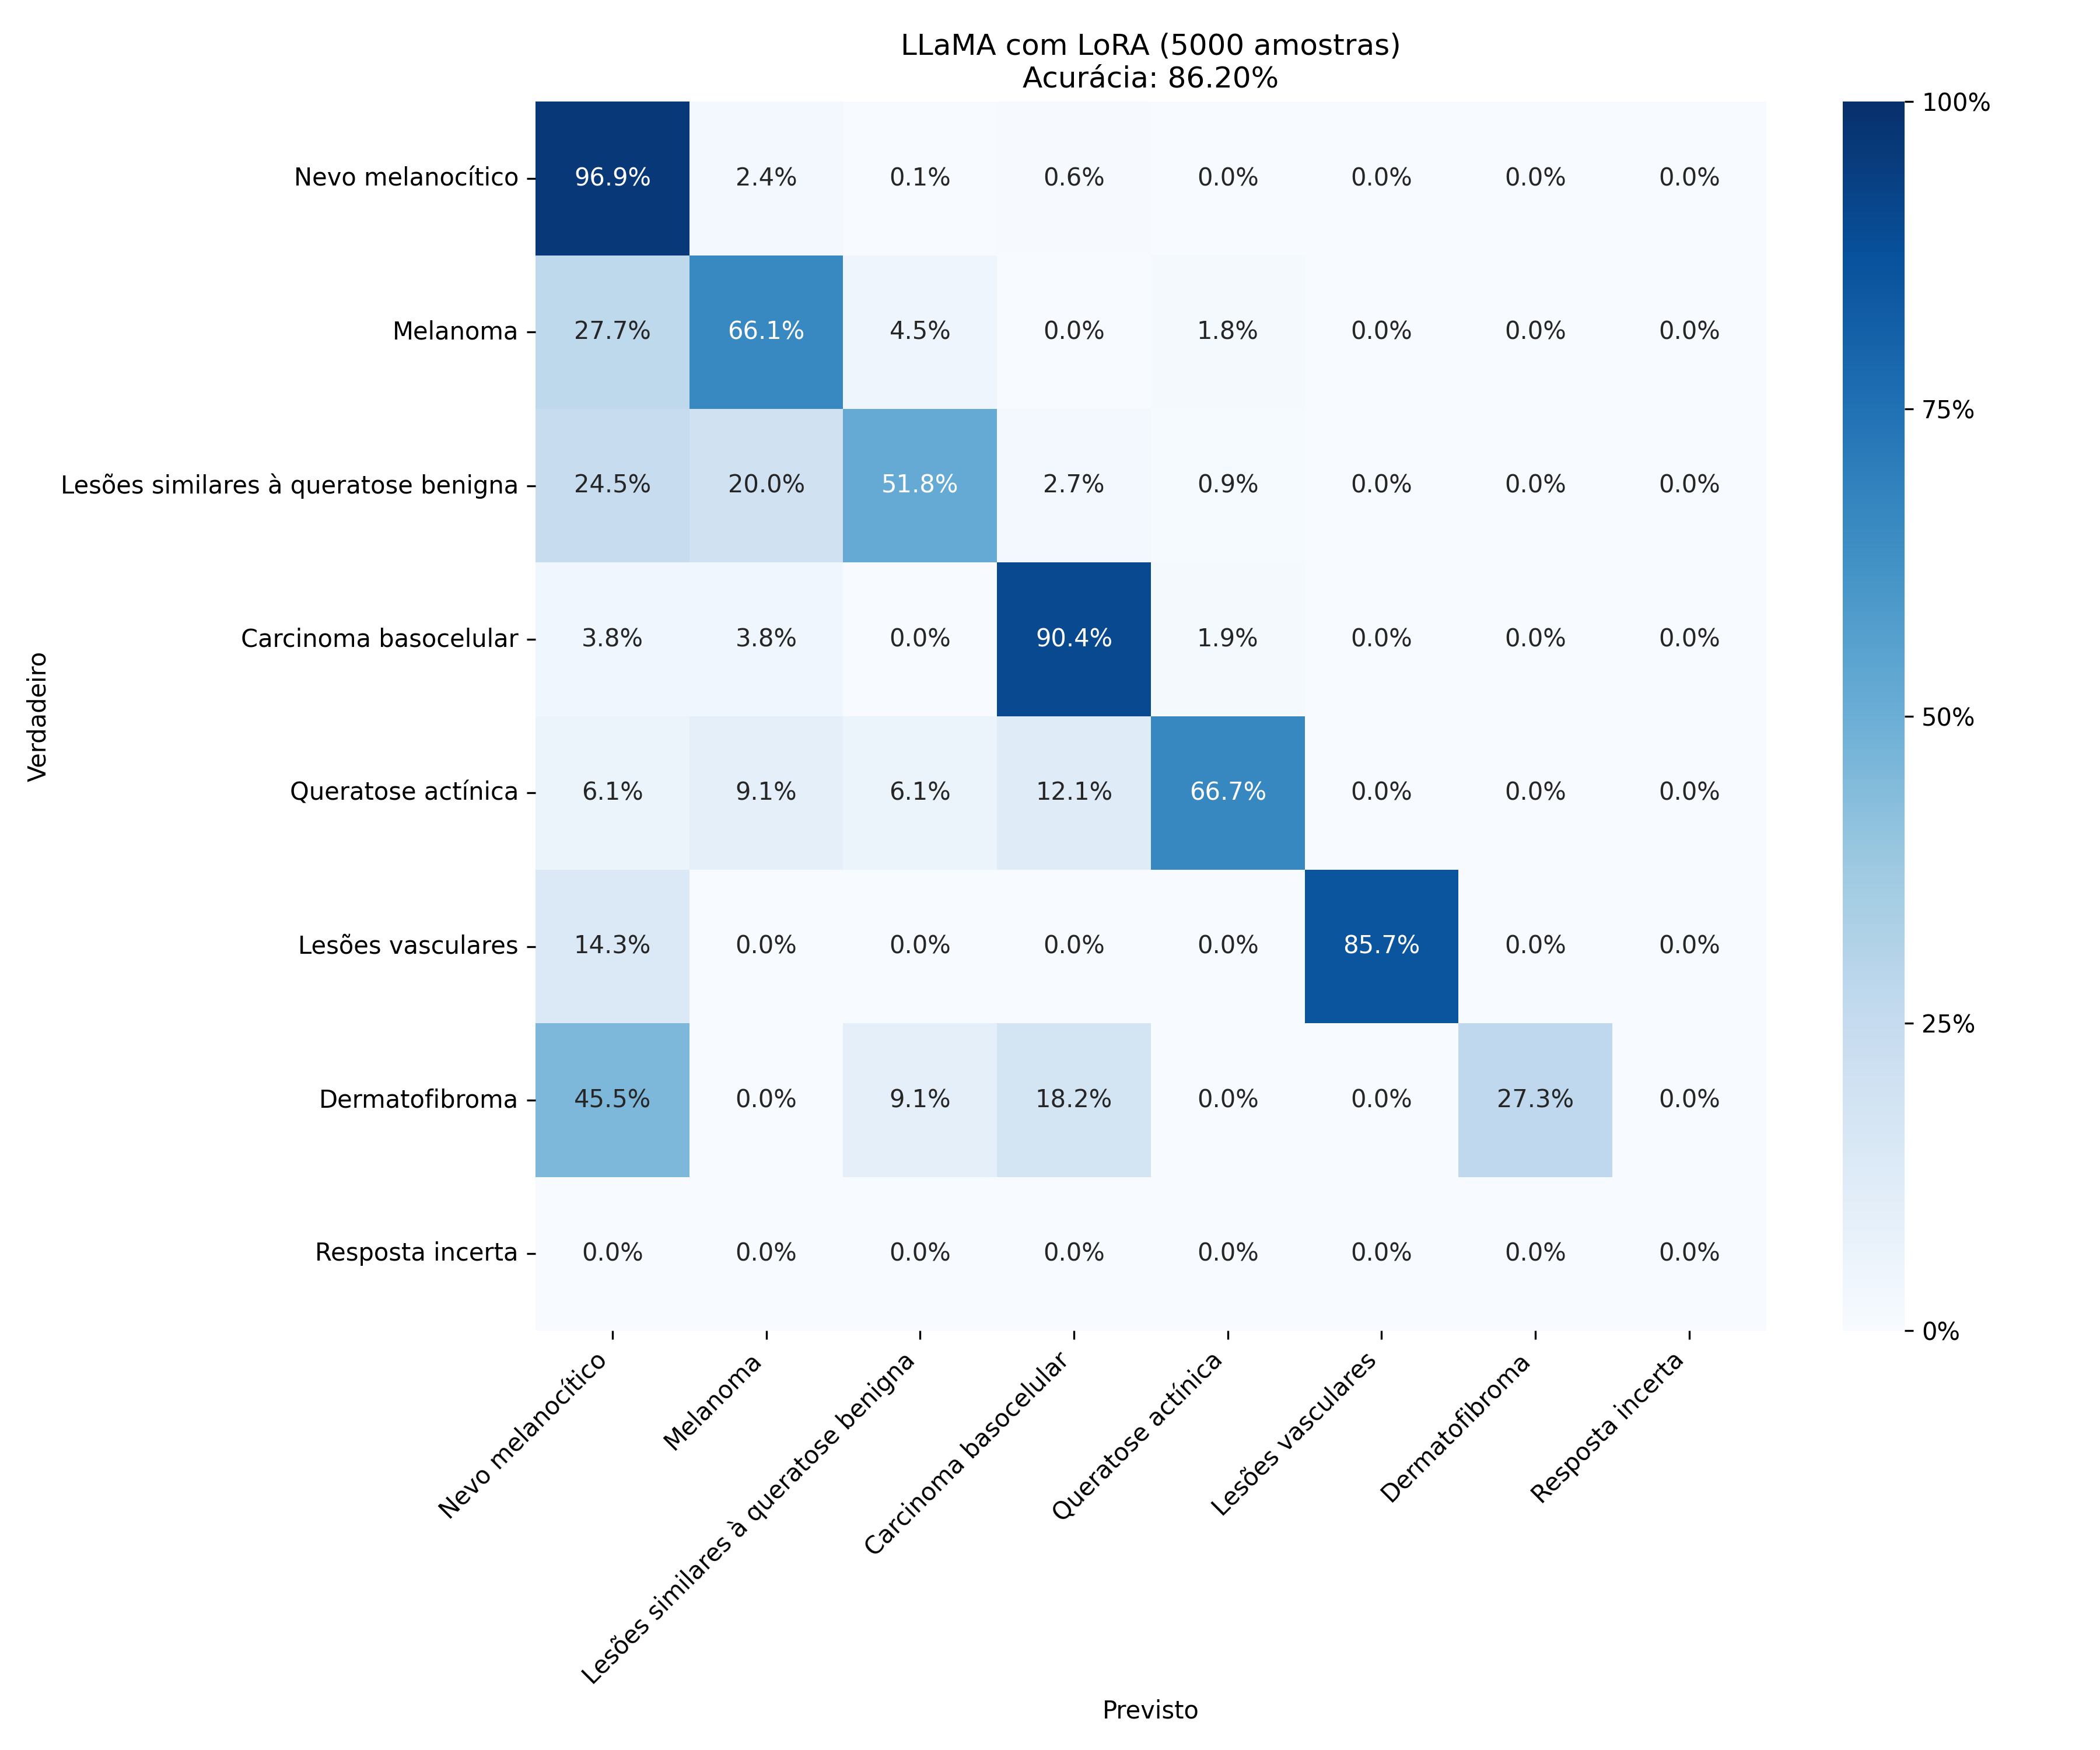
\includegraphics[width=1\columnwidth,keepaspectratio]{images/confusion_matrix_lora_5000.png}
    \label{fig:confusion_matrix_lora_5000}
    \fonte{Autoria própria.}
\end{figure}

Por último, o \ac{LLaMA} treinado com \ac{QLoRA} e 9500 amostras apresentou os melhores resultados, com uma acurácia de 87,4\%. A matriz de confusão pode ser vista na
\autoref{fig:confusion_matrix_qlora_9500}.

A \autoref{tab:training_accuracies} apresenta as acurácias de forma resumida.

\begin{figure}[ht]
    \centering
    \caption{\small Matriz de confusão para o \ac{LLaMA} treinado com \ac{QLoRA} e 9500 amostras.}
    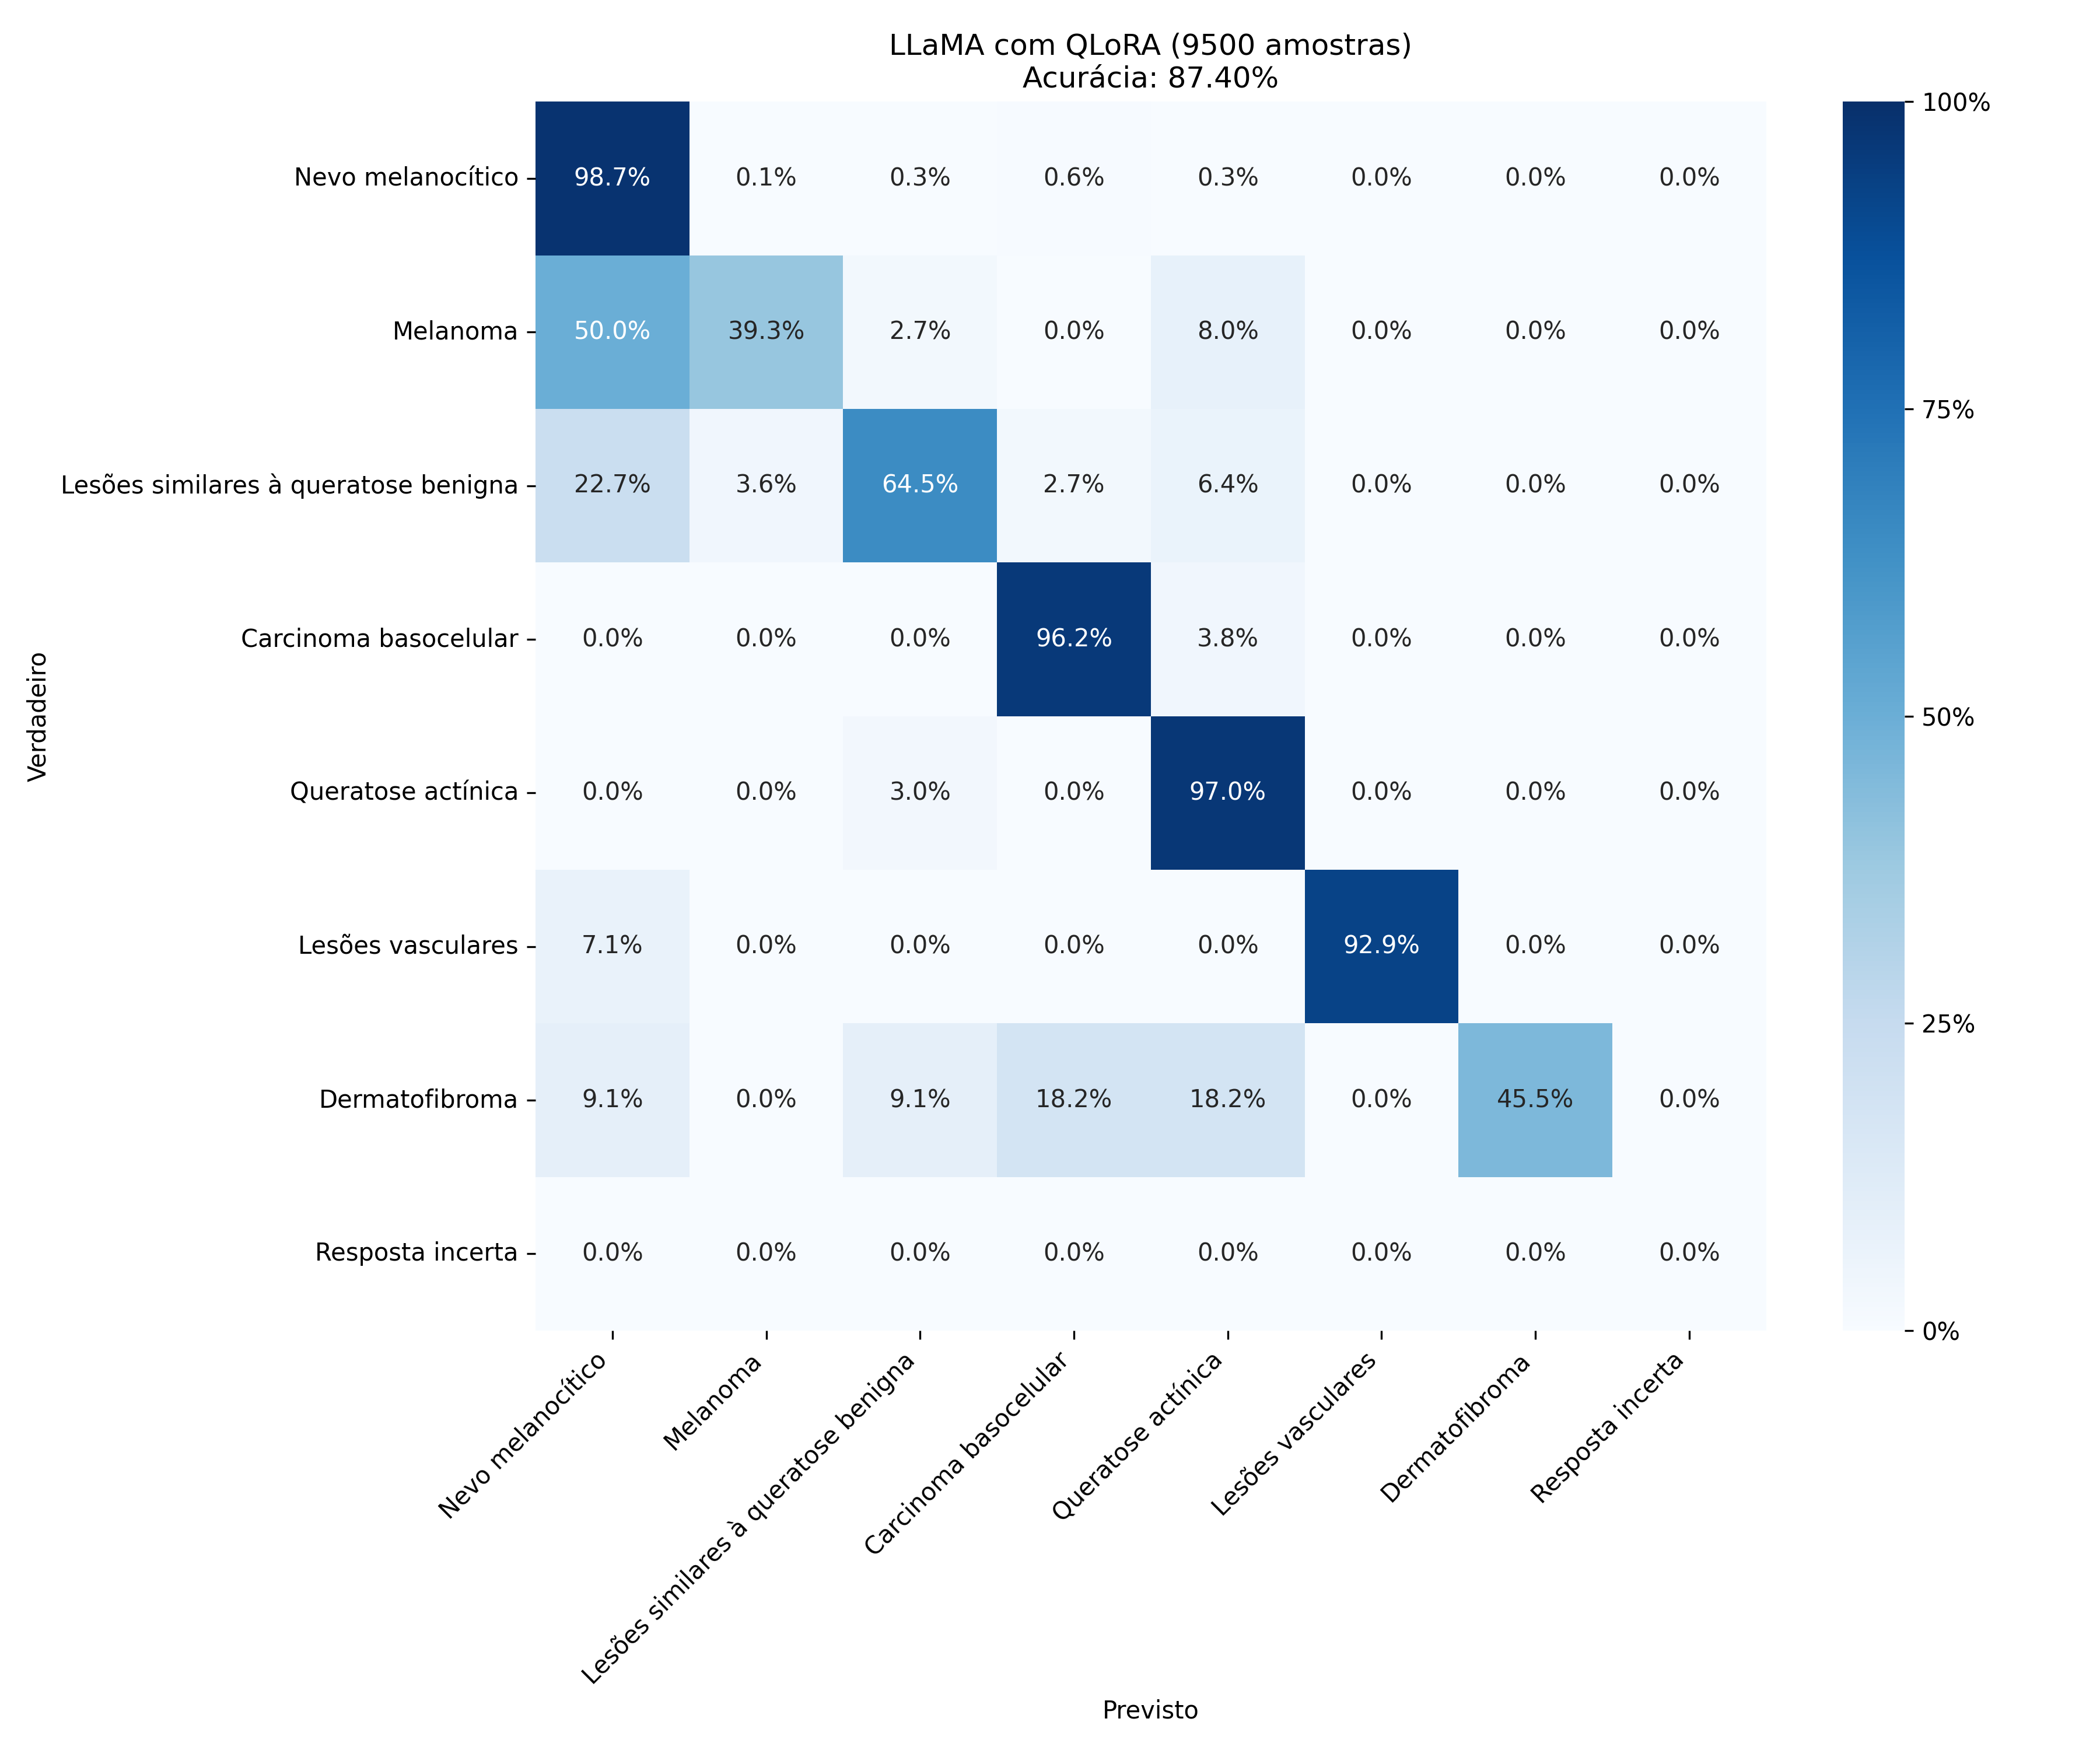
\includegraphics[width=1\columnwidth,keepaspectratio]{images/confusion_matrix_qlora_9500.png}
    \label{fig:confusion_matrix_qlora_9500}
    \fonte{Autoria própria.}
\end{figure}

\begin{table}[ht]
    \caption{\small Acurácia de cada modelo treinado.}
    \centering
    \begin{tabular}{l|c|c}
        \hline
        Método                      & Quantidade de amostras & Acurácia (\%) \\ \hline
        \multirow{5}{*}{\ac{QLoRA}} & 450                    & 65,5          \\
                                    & 900                    & 65,2          \\
                                    & 1800                   & 71,1          \\
                                    & 5000                   & 85,4          \\
                                    & 9500                   & 87,4          \\ \hline
        \multirow{3}{*}{\ac{LoRA}}  & 450                    & 49,5          \\
                                    & 900                    & 42,0          \\
                                    & 5000                   & 86,2          \\ \hline
    \end{tabular}
    \label{tab:training_accuracies}
    \fonte{Autoria própria}
\end{table}

%\phantompart
\chapter{Conclusões Parciais e Planejamento}

...


% Elementos pós-textuais
\postextual

% Referências bibliográficas
\begingroup
\printbibliography[title=REFERÊNCIAS]
\endgroup

% Apêndices
%\begin{apendicesenv}
%	\partapendices* 
%	% ----------------------------------------------------------
\chapter{Descrição}
% ----------------------------------------------------------

Textos elaborados pelo autor, a fim de completar a sua argumentação. Deve ser precedido da palavra APÊNDICE, identificada por letras maiúsculas consecutivas, travessão e pelo respectivo título. Utilizam-se letras maiúsculas dobradas quando esgotadas as letras do alfabeto.

\begin{quadro}[htb]
    \centering
    \caption{\label{qua:Quadro_2}Modelo A.}
    \begin{tabular}{|l|l|}
        \hline
        xxxx              & yyyyyyyyyyyyyyy    \\
        \hline
        xxxx              & yyyyyyyyyyyyyyy    \\
        \hline
        xxxx              & yyyyyyyyyyyyyyy    \\
        \hline
        xxxx              & yyyyyyyyyyyyyyy    \\
        \hline
        xxxx              & yyyyyyyyyyyyyyy    \\
        \hline
        xxxx              & yyyyyyyyyyyyyyy    \\
        \hline
        xxxx              & yyyyyyyyyyyyyyy    \\
        \hline
        rrrrrrrrrrrrrrrrr & eeeeeeeeeeeeeeeee  \\
        \hline
        xxxx              & yyyyyyyyyyyyyyy    \\
        \hline
        xxxx              & yyyyyyyyyyyyyyy    \\
        \hline
        rrrrrrrrrrrrrrrrr & eeeeeeeeeeeeeeeee  \\
        \hline
        xxxx              & yyyyyyyyyyyyyyy    \\
        \hline
                          & ttttttttttttttttt  \\
        \hline
        rrrrrrrrrrrrrrrrr & eeeeeeeeeeeeeeeee  \\
        \hline
        ttttttttttttt     &                    \\
        \hline
        rrrrrrrrrrrrrrrrr & eeeeeeeeeeeeeeeee  \\
        \hline
        rrrrrrrrrrrrrrrrr & eeeeeeeeeeeeeeeee  \\
        \hline
                          & gggggggggggggggggg \\
        \hline
        rrrrrrrrrrrrrrrrr & eeeeeeeeeeeeeeeee  \\
        \hline
        rrrrrrrrrrrrrrrrr & eeeeeeeeeeeeeeeee  \\
        \hline
        rrrrrrrrrrrrrrrrr & eeeeeeeeeeeeeeeee  \\
        \hline
        rrrrrrrrrrrrrrrrr & eeeeeeeeeeeeeeeee  \\
        \hline
    \end{tabular}
    \fonte{Elaborada pelo autor (2016).}
\end{quadro}
%\end{apendicesenv}

\end{document}
